% !TEX TS-program = pdflatex
% !TEX encoding = UTF-8 Unicode

\documentclass[czech,master,public,dept460,male,java,cpdeclaration]{diploma}
%\documentclass{article}

\usepackage[czech]{babel}
\usepackage[T1]{fontenc}
\usepackage[utf8]{inputenc}
\usepackage{color}
\usepackage{geometry}
\usepackage{float}
\usepackage{graphicx}
\usepackage[stable]{footmisc}
\usepackage{hyperref}
\usepackage{amsfonts}
\usepackage{amsmath}
 \usepackage{bbm}
 \usepackage{booktabs}
 \usepackage{url}
 \usepackage{nameref}
 \usepackage{caption}
 \usepackage{subcaption}
 \usepackage{listings}
\renewcommand{\baselinestretch}{1.2}
 \ThesisAuthor{Josef Raška}

% U bakalarske praxe neni nutne nazev zadavat
\CzechThesisTitle{Mobilní aplikace pro usnadnění cestování uživatelům s mentálním postižením}


% U bakalarske prace neni nutne anglicky nazev zadavat
\EnglishThesisTitle{Mobile Applications to Facilitate Travelling for Users with Mental Disabilities}

\SubmissionDate{29. dubna 2016}

\Thanks{Rád bych poděkoval mému vedoucímu Ing. Janu Martinovičovi, Ph.D. za pomoc, připomínky a vedení této práce.

Dále děkuji paní Mgr. Barboře Uhlířové ze společnosti SPMP za konzultace a pomoc při formulaci zadání.}

\CzechAbstract{Cílem práce je analyzovat problémy, se kterými se setkávají lidé s mentálním postižením
při jejich každodenním cestování, vymyslet a implementovat za pomoci dostupných
nástrojů mobilní aplikaci na platformu Android, řešící tyto úkony
a následně ji publikovat a otestovat.
V rámci práce byla navržena a vyvinuta Android aplikace pro asistenci cestování, která by měla lidem
 s mentálním postižením usnadnit jejich obvyklé cesty, poskytnout jim prostředek pro jejich uchovávání
  a urychlit komunikaci s jejich asistentem. Aplikace využívá pro asistenci systému GPS, pro efektivní
  implementaci množství aktuálních knihoven, postupů a pro zjednodušené zrychlené zadávání vstupu do aplikace
  byla využita technologie NFC.
 Výsledná aplikace byla publikována do obchodu Google Play a následně otestována v městském prostředí, kde
  uživatelům může přinést požadovanou pomoc. Implementace má volně přístupné zdrojové kódy a ty tak mohou být
  zdrojem pro její další rozvoj a širšímu využití.}


\CzechKeywords{Android, vývoj, asistence cestování, mobilní aplikace, mentální postižení, aplikační návrh,
GPS, NFC, Google Play, GitHub}

\EnglishAbstract{The aim of the thesis is to analyze problems, which the people with mental
disabilities deal with during every day traveling, invent and implement mobile
application on Android platform with available tools, which will solve these issues, then publish and test it.
Android application for travel asistance was designed and developed as part of this thesis, which should help the people
with mental disabilities make their usual travels easier, provide them tool for saving them and speed up
communication with their assistant. Application uses GPS system for assistace, lot of actual libraries
and methodologies for effective implementation and NFC technology was used for faster and easier input actions.
Application was published to Google Play store and then tested in city environment, where the users can benefit
from it. Implementation is completely open source and the code could be source for its next development and
broader usage.
}

\EnglishKeywords{Android, development, travel asistance, mobile application, mental disabilities, application design,
GPS, NFC, Google Play, GitHub}

\AddAcronym{SDK}{Software development kit (\textit{Soubor nástrojů pro vývoj})}
\AddAcronym{GPS}{Global Positioning System (\textit{Globální systém určování polohy})}
\AddAcronym{NFC}{Near field communication (\textit{Technologie pro přenos dat})}
\AddAcronym{API}{Application programming interface
\newline (\textit{Rozhraní pro programování aplikací})}

\AddAcronym{UML}{Unified Modeling Language
\newline (\textit{Grafický jazyk v softwarovém inženýrství})}

\AddAcronym{SD karta}{Paměťová karta technologie Secure Digital}
\AddAcronym{ORM}{Objektově relační mapování}
\AddAcronym{ZIP}{Souborový formát pro kompresi a archivaci dat}
\AddAcronym{HTTP}{Hypertext Transfer Protocol
\newline (\textit{Protokol pro přenos webových dokumentů})}

\AddAcronym{REST}{Representational State Transfer
\newline (\textit{Architektura rozhraní HTTP komunikace})}

\AddAcronym{SOLID}{Single responsibility, open-closed, Liskov substitution principle, interface segregation and dependency inversion
(\textit{Jedna odpovědnost, otevřenost k rozšíření, uzavřenost ke změnám, princip Liskové substituce,
oddělení rozhraní a obrácení závislostí})}
\AddAcronym{IoC}{Inversion of control (\textit{Obrácení závislostí})}
\AddAcronym{MVC}{Model View Controller (\textit{Typ architektury aplikací})}
\AddAcronym{MVP}{Model View Presenter (\textit{Typ architektury aplikací})}



%\ThesisAssignmentImagePath{Figures/Zadani}

% Zadame soubor s digitalizovanou podobou prohlaseni
% Pokud toto makro zapoznamkujeme sazi se cisty text prohlaseni
\AuthorDeclarationImageFile{img/declaration.jpg}
\CooperatingPersonsDeclarationImageFile{img/publicationagreement.jpg}


\renewcommand{\lstlistingname}{Ukázka kódu}
\renewcommand{\lstlistlistingname}{List of ukázek kódu s}

\usepackage{inconsolata}
\lstset{ %
%  backgroundcolor=\color{white},   % choose the background color; you must add \usepackage{color} or \usepackage{xcolor}
  basicstyle=\footnotesize\color{black},        % the size of the fonts that are used for the code
%  breakatwhitespace=false,         % sets if automatic breaks should only happen at whitespace
%  breaklines=true,                 % sets automatic line breaking
  captionpos=b,                    % sets the caption-position to bottom
%  commentstyle=\color{mygreen},    % comment style
%  deletekeywords={...},            % if you want to delete keywords from the given language
%  escapeinside={\%*}{*)},          % if you want to add LaTeX within your code
%  extendedchars=true,              % lets you use non-ASCII characters; for 8-bits encodings only, does not work with UTF-8
  frame=single,	                   % adds a frame around the code
  keepspaces=true,                 % keeps spaces in text, useful for keeping indentation of code (possibly needs columns=flexible)
  keywordstyle=\color{blue},       % keyword style
  identifierstyle=\color{black},
  language=Java,                 % the language of the code
%  otherkeywords={*,...},           % if you want to add more keywords to the set
 inputencoding=utf8,
  numbers=none,                    % where to put the line-numbers; possible values are (none, left, right)
%  numbersep=5pt,                   % how far the line-numbers are from the code
%  numberstyle=\tiny\color{mygray}, % the style that is used for the line-numbers
  rulecolor=\color{black},         % if not set, the frame-color may be changed on line-breaks within not-black text (e.g. comments (green here))
%  showspaces=false,                % show spaces everywhere adding particular underscores; it overrides 'showstringspaces'
%  showstringspaces=false,          % underline spaces within strings only
  showtabs=false,                  % show tabs within strings adding particular underscores
%  stepnumber=2,                    % the step between two line-numbers. If it's 1, each line will be numbered
%  stringstyle=\color{mymauve},     % string literal style
  tabsize=2,	                   % sets default tabsize to 2 spaces
  literate={á}{{\'a}}1 {é}{{\'e}}1  {č}{{\'c}}1 {ý}{{\'y}}1 {í}{{\'i}}1 {ú}{{\'u}}1 {▼}{$\downarrow{}$}{1},
%  title=\lstname                   % show the filename of files included with \lstinputlisting; also try caption instead of title
}

\title{Diplomová práce}
\author{Josef Raška \(ras0029\)}
\newtheorem{priklad}{Příklad}[section]
\newtheorem{veta}{Věta}[section]
\newtheorem{alg}{Algoritmus}[section]

\newcommand{\usecase}[2]{\subsubsection{#1}\label{#2}}
\setcounter{tocdepth}{2}

\begin{document}
%\maketitle
\MakeTitlePages
\urlstyle{same}

%\tableofcontents
%\listoffigures
%\listoftables
%\lstlistoflistings

\newpage

\section{Úvod}
Problém cestování a orientace v reálném čase je v dnešním světě občas složitým problémem pro nás všechny,
pro lidi s mentálním postižením pak problémem mnohonásobným. Cesta do zaměstnání, do banky
nebo jen do obchodu může být pro člověka s mentálním postižením velmi těžký úkol, jelikož často musí
využít hromadné dopravy, přecházet složité křižovatky a podobně. Lidí s mentálním postižením
je momentálně v České republice více než 100 tisíc\cite{komunikace} a jedná se tedy o velice
významnou skupinu, která si zaslouží zvláštní pozornost. Tito lidé pak při svém cestování často potřebují
pomoc asistenta, kterých je však pro takto početnou skupinu nedostatek.
Dnes jsou již chytré mobilní telefony poměrně snadno dostupnou věcí, spoustu lidí
s mentálním postižením tyto telefony více než zdatně ovládá a nabízí se tedy možnost pokusit se prostřednictvím
 této techniky těmto lidem pomoci. V tomto případě mobilními zařízeními se systémem Android,
 který je v současné době nejrozšířenějším a také nejdostupnějším mobilním operačním systémem.

 Jako téma mé diplomové práce jsem si proto vybral vytvoření mobilní aplikace pro mentálně postižené,
 která se pokusí usnadnit jim cestování a urychlit komunikaci s asistentem. V práci se nejprve
 seznámíme s procesem vytváření zadání aplikace na základě podrobné diskuze k dané problematice s povolanými osobami,
 dále si představíme funkční a grafický návrh aplikace a samotnou platformu Android.
 Následovat pak bude popis implementace za použití aktuálních nástrojů a knihoven, kde může práce sloužit
 i jako přehled aktuálních trendů vývoje Android aplikací a následně ukážeme, jak je možné aplikaci propojit
 se službami třetích stran pro rozšíření její funkcionality, jak
 můžeme aplikaci publikovat a zpřístupnit ji snadno uživatelům. Závěrem budou popsány
 změny a úpravy provedené po obdržení zpětné vazby
a případné možnosti dalšího vývoje tohoto typu aplikace.


\section{Návrh aplikace}
Mentální postižení není nemoc, je to trvalý stav, který se projeví do 18 let věku a nedá se léčit\cite{komunikace}.
U každého člověka s mentálním postižením se jeho stav projevuje jinak a je proto potřeba k nim
přistupovat individuálně. Tito lidé mají často potíže s učením, porozuměním, sníženou míru pozornosti
a horší orientaci v čase a prostoru\cite{komunikace}, což je pro spolehlivé cestování důležité.
Aplikace byla navrhována s přihlédnutím k těmto faktům a v každé její části jsme se snažili o co nejjednodušší
vzhled aplikace a její ovládání.


\subsection{Příprava zadání}
Na začátku práce bylo potřeba stanovit si cíle a zjistit, jaká úskalí vlastně lidé s mentálním
postižením při cestování zažívají, s jakými problémy se potýkají a co by pro ně mohlo být přínosné.

Úvodní konzultace byly vedeny s paní Mgr. Barborou Uhlířovou z Brněnského poradenského centra
Společnosti pro podporu lidí s mentálním postižením v České republice, z.s. Od paní Uhlířové jsem
získal cenné rady, jak postupovat a zdroje, které mi pomohly lépe pochopit, jak se k mentálně postiženým chovat,
 co od nich očekávat a jak k nim, jako k uživatelům mobilní aplikace přistupovat.

Po první konzultaci byly vytvořeny návrhy, co by mohla aplikace dělat a tyto návrhy byly diskutovány.
Po další emailové komunikaci jsme se s paní Uhlířovou dohodli, že pro ještě lepší zadání bude
dobré konzultovat nápady s jejími kolegy v Brně a začalo se připravovat setkání, které se následně
v Brně uskutečnilo a zúčastnilo se ho asi deset pečovatelů různých věkových kategorií a také dva klienti
sdružení.

Návrhy jim byly prezentovány a po diskuzi a zpětné vazbě byli ve spolupráci s mým vedoucím definováni
aktéři aplikace a vytvořena sada případů užití(use casů), které dávají pro toto zadání smysl a následně
budou mnohé z nich implementovány.

\subsection{Popis aktérů}
\begin{figure}[H]
        \centering
                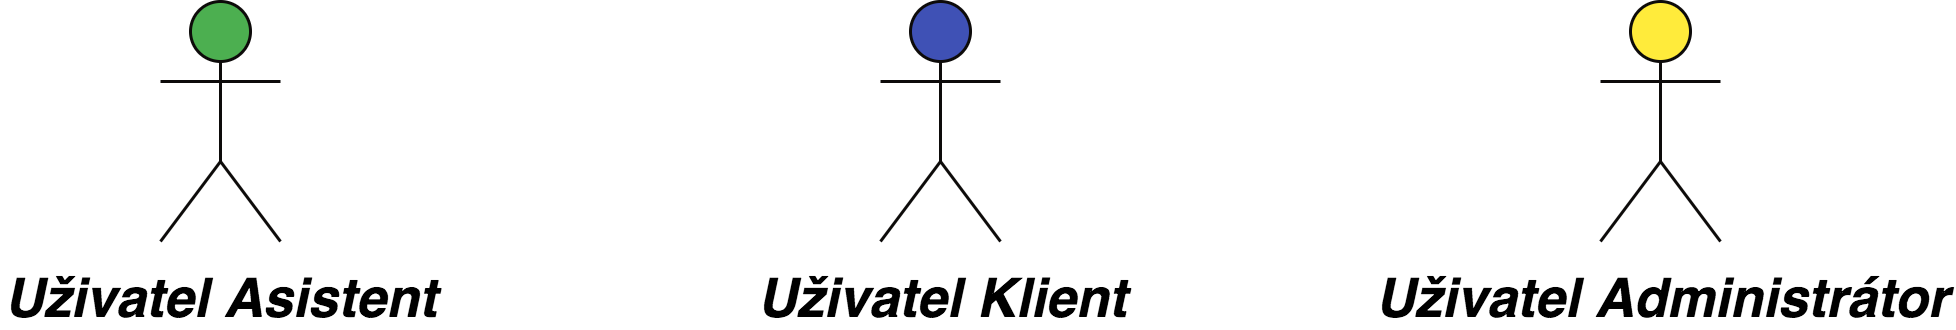
\includegraphics[scale=0.14]{img/actors.png}
        \caption{Aktéři systému}
        \label{fig:actors}
\end{figure}

Pro uživatele klienta i asistenta jsou definovány případy užití zvlášť, neboť se celé chování
a použití aplikace bude v obou případech značně lišit. Grafické zobrazení aktérů je na obrázku~\ref{fig:actors}.
Pro ilustraci případů užití jednotlivých aktérů jsou použity obrázky z reálné aplikace pro
lepší přiblížení a popis daného use casu.

\subsubsection{Uživatel Asistent}
Jedná se o aktéra, který je zároveň klientovi s mentálním postižením odborným asistentem,
jenž o něj pečuje a poskytuje mu podporu. Tento aktér je relevantní k vytváření obsahu,
který má pomoci klientovi k lepší orientaci při cestování a také mu může připravenou
cestu předvést. Může také nahraná data editovat a případně je rozšiřovat. Může také zadat
do aplikace zadat své kontaktní údaje pro možnou nečekanou situaci klienta na cestách, případně
nastavit zálohování uložených dat pro zamezení jejich ztráty při ztrátě telefonu nebo jeho výměně
za jiný.

\subsubsection{Uživatel Klient}
Klient je osoba pro kterou je aplikace primárně určena a má mu pomoci vyřešit problém,
v tomto případě pomoci z orientací při cestování. Může si prohlížet obsah a zejména ho
využívat při cestách v terénu. Uživatel by měl být upozorněn na všechny uložené a rozeznané
data v závislosti na své pozici a měl by tak získat relevantní informace k tomu, kde se právě
nachází. Dále může aplikaci využít ke snadnému kontaktování svého asistenta.


\subsubsection{Uživatel Administrátor}
Administrátor může být spravující asistent, případně jiná osoba, která je oprávněna spravovat
data nahraná ostatními asistenty a využívána klienty. Může tyto záznamy prohlížet a případně
 upravovat a ovlivnit tak co se kterému uživateli zobrazí a jakým způsobem bude asistence probíhat.


\subsection{Use casy uživatel Asistent}
Pro uživatele asistenta jsou určeny složitější operace pro vytváření interaktivního obsahu pro klienta,
nastavování aplikace a prezentace klientovi. Pro use casy asistenta platí, že klient může těmto
krokům přihlížet, pokud o to projeví zájem. Use casy asistenta a jejich vztahy lze vidět na obrázku~\ref{fig:UseCasesAsistant}.

\begin{figure}[H]
        \centering
                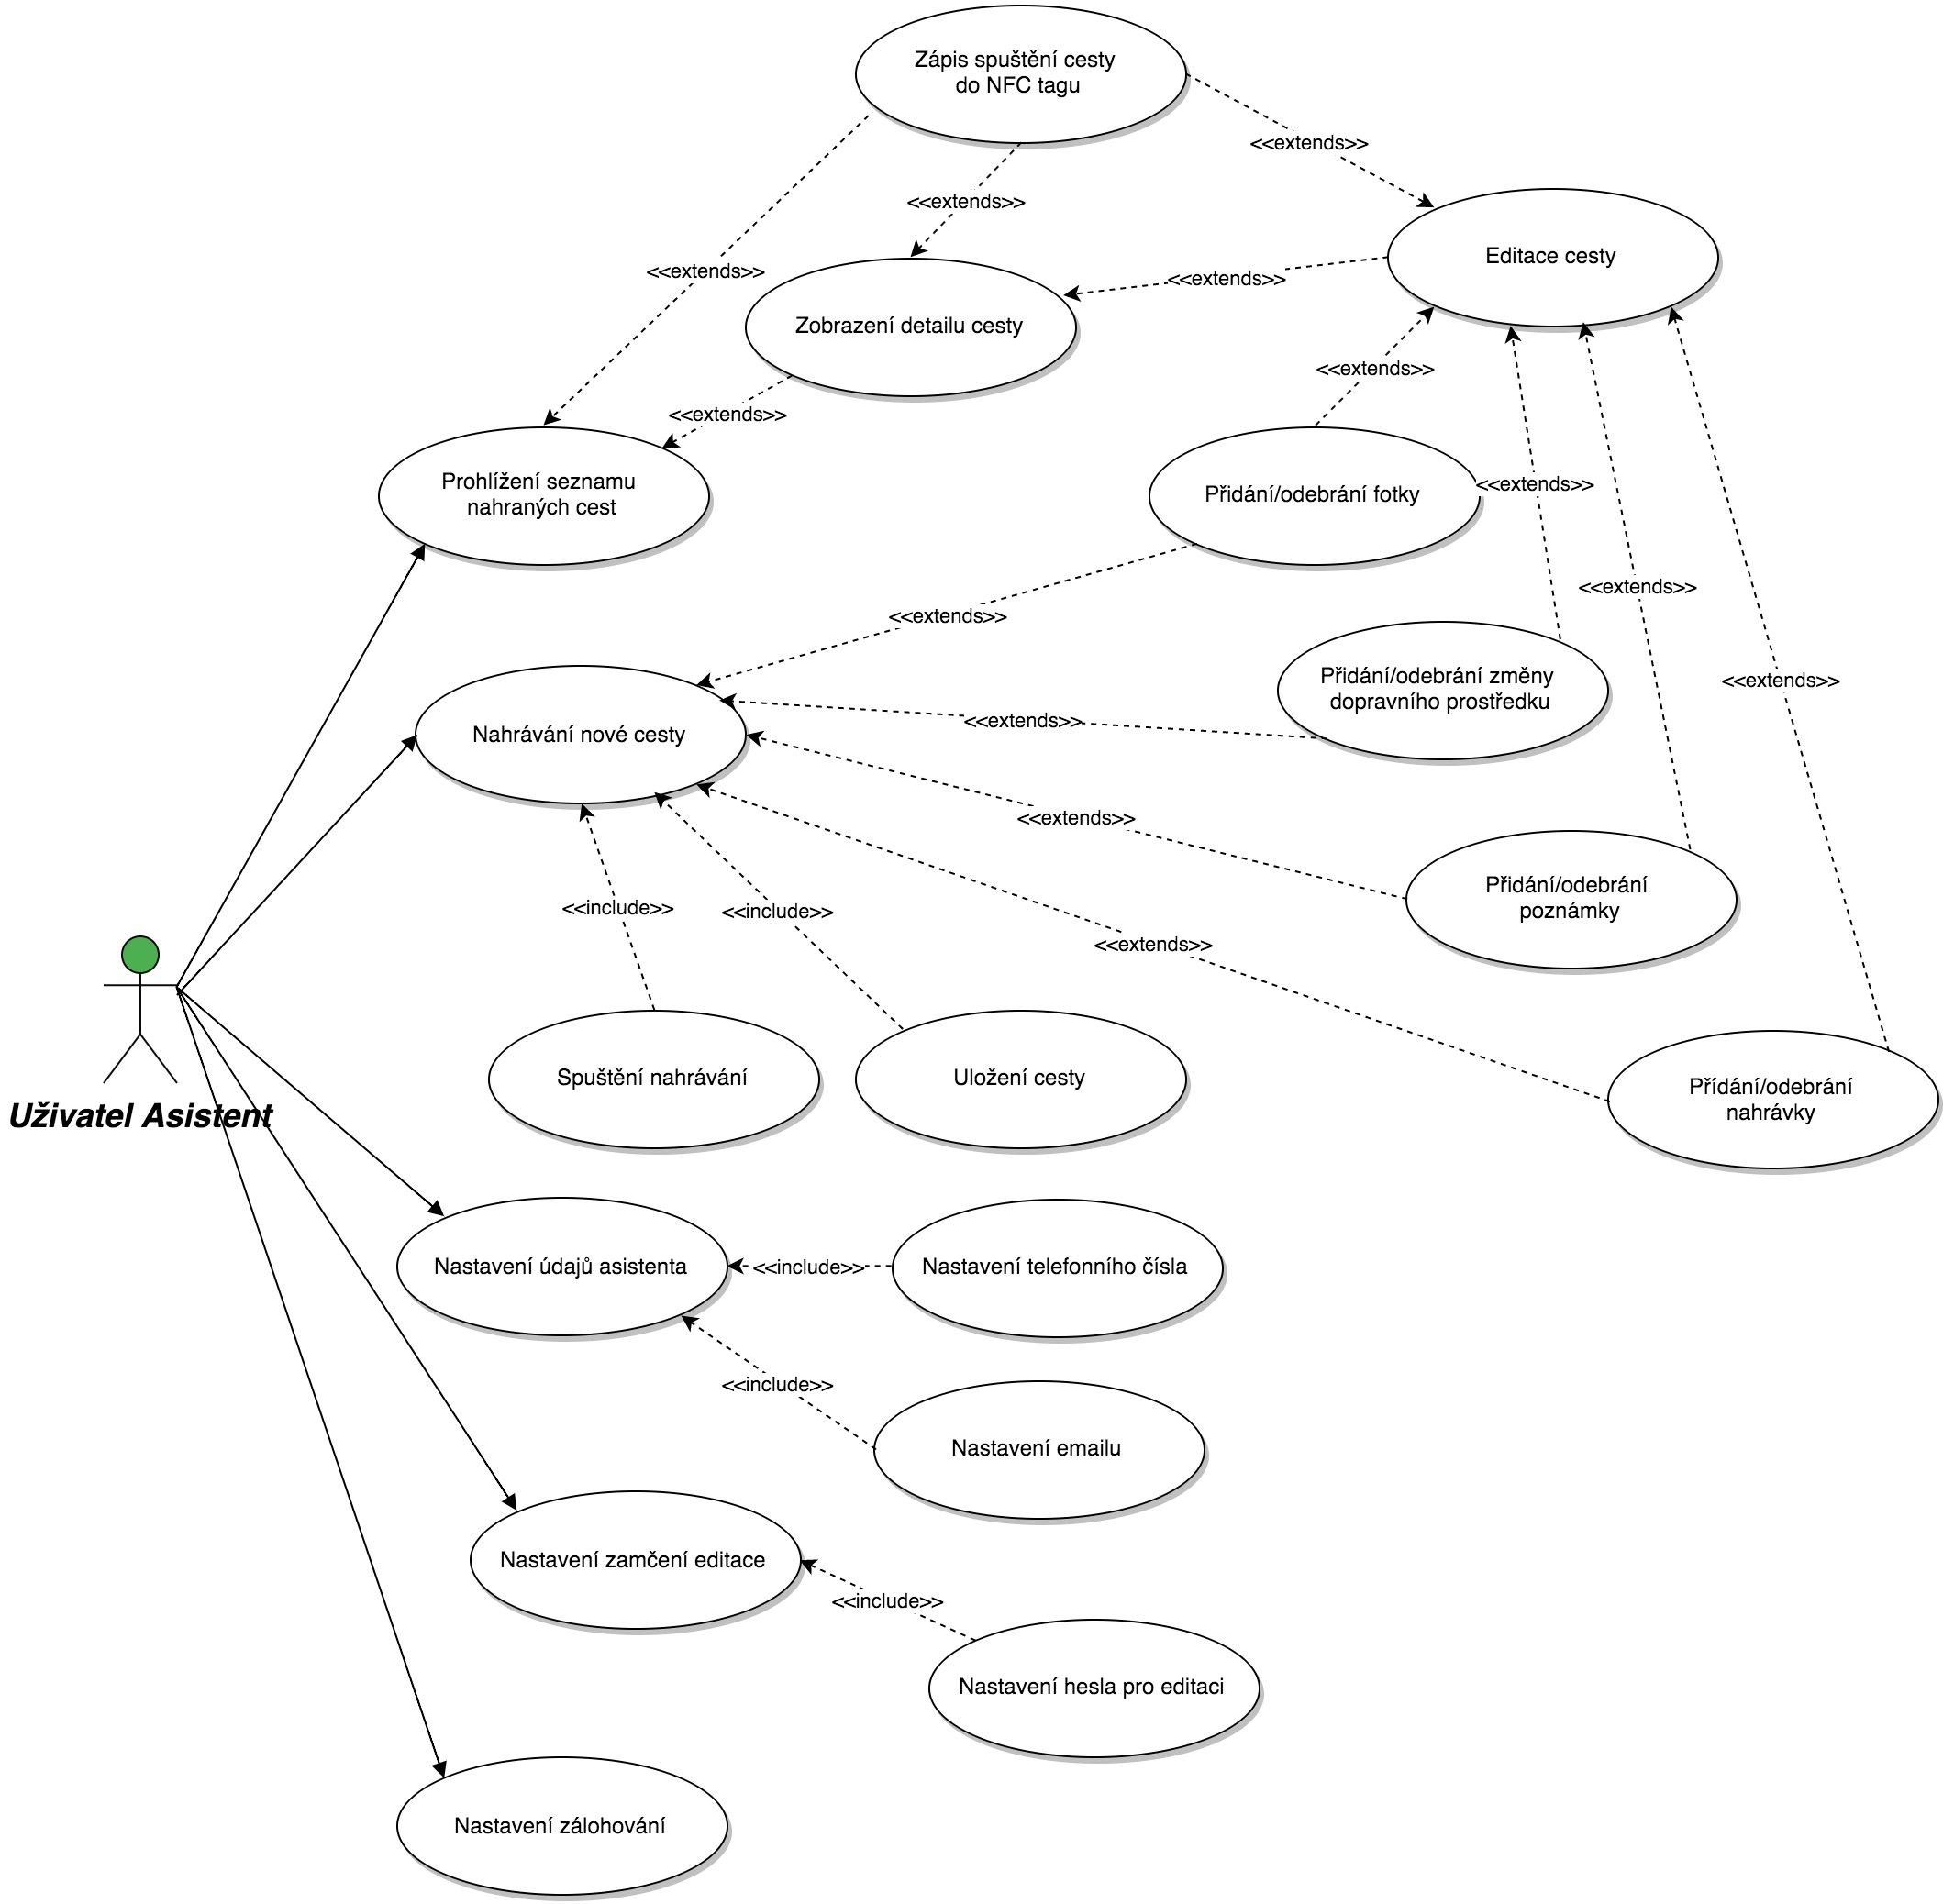
\includegraphics[scale=0.2]{img/UseCasesAsistant.png}
        \caption{Diagram use casů uživatele asistent}
        \label{fig:UseCasesAsistant}
\end{figure}

\usecase{Prohlížení seznamu nahraných cest}{prohlizeniasistent}
\textbf{Aktéři:} Asistent

\vspace{0.1cm}
\noindent
\textbf{Hlavní scénář:} Na úvodní obrazovce jsou zobrazeny všechny dosud nahrané cesty ve seznamu pod sebou.
Lze vidět pouze základní údaje a přiřazený obrázek pro snadnou orientaci. Uživatel se pomocí
kliknutí na řádek může podívat na celý detail cesty, případně pomocí rychlých akcí spustit ihned asistenci
a podobně. Obrazovku prohlížení cest lze vidět na obrázku~\ref{fig:prohlizeniasistent}.

\vspace{0.1cm}
\noindent
\textbf{Spouštěč:} Uživatel spustí aplikaci nebo se do ní vrátí pomocí notifikace v liště upozornění.

\vspace{0.1cm}
\noindent
\textbf{Rozšíření:}
\begin{itemize}
  \item \nameref{nahravanicesty}
  \item \nameref{detailasistent}
  \item \nameref{nfczapis}
\end{itemize}

\begin{figure}[H]
\begin{minipage}{.5\textwidth}
\centering
                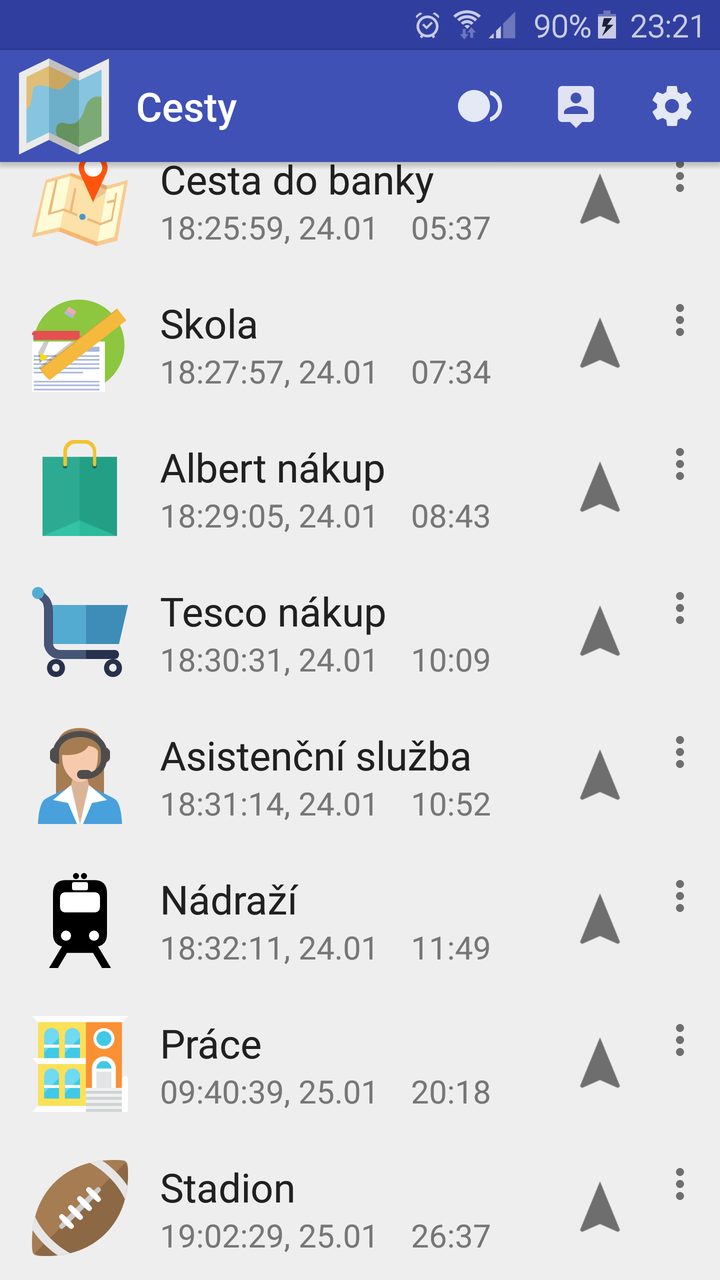
\includegraphics[scale=0.14]{img/screen/seznamcest.png}
        \caption{Prohlížení seznamu cest}
        \label{fig:prohlizeniasistent}
\end{minipage}
\begin{minipage}{.5\textwidth}
    \centering
                    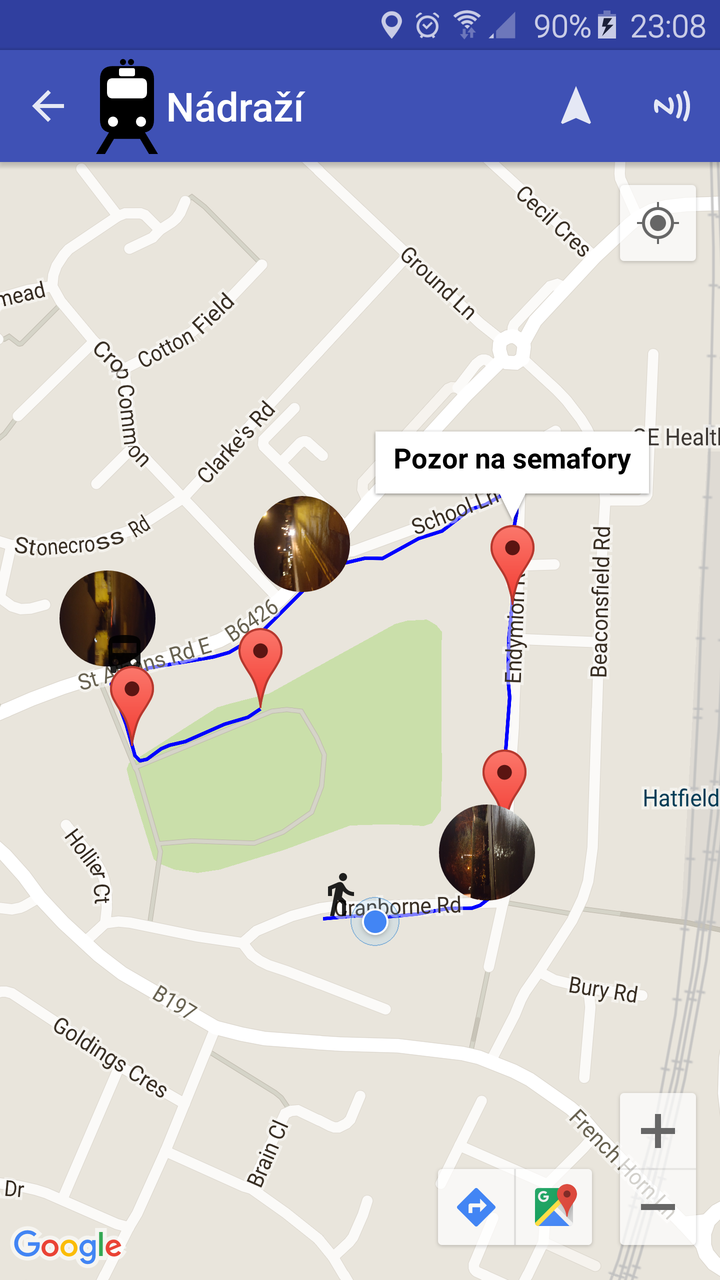
\includegraphics[scale=0.14]{img/screen/detailcesty.png}
            \caption{Zobrazení detailu cesty}
            \label{fig:detailasistent}

       \end{minipage}
\end{figure}

\usecase{Zobrazení detailu cesty}{detailasistent}
\textbf{Aktéři:} Asistent

\vspace{0.1cm}
\noindent
\textbf{Hlavní scénář:} Uživateli se zobrazí detail cesty se všemi informacemi, které jsou o ní uloženy.
Na mapě si může prohlédnout kudy vedla, na místech pořízení fotografií jsou miniatury fotek, při změně dopravních
prostředků lze vidět ikony daných prostředků, zvukově a textové záznamy jsou označeny příslušnou ikonou.
Při klepnutí na indikátor některého z těchto záznamů se zobrazí jeho popis, který uživatel dříve zadal.
V detailu cesty lze poklepáním na tlačítko editovat přejít do módu editace cesty a všechny dříve zmíněné
záznamy upravit. Ukázku lze vidět na obrázku~\ref{fig:detailasistent}.

\vspace{0.1cm}
\noindent
\textbf{Prekondice:} Cesta je uložena.

\vspace{0.1cm}
\noindent
\textbf{Spouštěč:} Uživatel klepne na řádek se zobrazenou cestou v seznamu cest.

\vspace{0.1cm}
\noindent
\textbf{Rozšíření:}
\begin{itemize}
  \item \nameref{editacecesty}
  \item \nameref{nfczapis}
\end{itemize}






\usecase{Zapsání cesty do NFC tagu}{nfczapis}
\textbf{Aktéři:} Asistent

\vspace{0.1cm}
\noindent
\textbf{Hlavní scénář:} Uživateli se zobrazí
obrazovka, která jej instruuje k přiložení NFC tagu k telefonu. Jakmile telefon zaznamená blízkost tagu,
zapíše do něj informaci o uložené cestě pro následné rychlé spouštění při přiložení tagu k telefonu.
Obrazovku zápisu do NFC tagu lze vidět na obrázku~\ref{fig:nfczapis} a oznámení o zapsaném tagu
na obrázku~\ref{fig:nfczapsano}.

\vspace{0.1cm}
\noindent
\textbf{Prekondice:} Cesta je uložena.

\vspace{0.1cm}
\noindent
\textbf{Spouštěč:} Uživatel klepne na ikonu NFC v detailu cesty nebo na rozšiřující menu v seznamu cest.


\begin{figure}[H]
\begin{minipage}{.5\textwidth}
\centering
                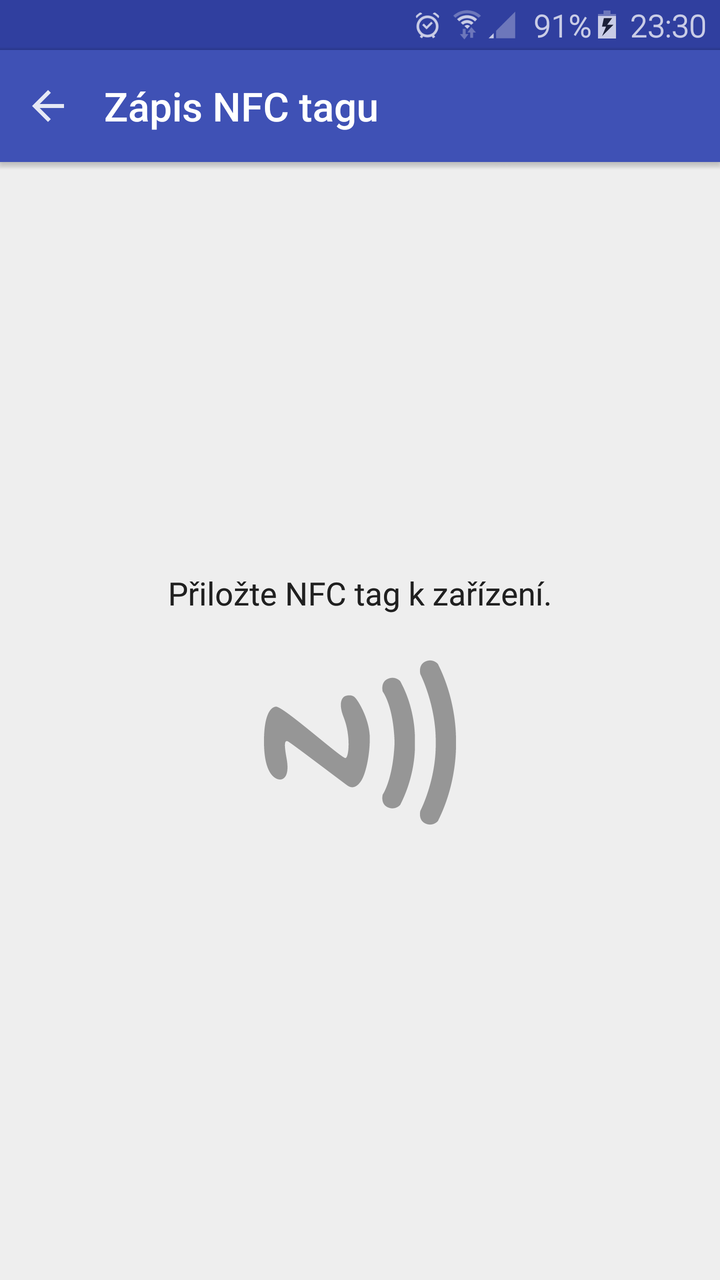
\includegraphics[scale=0.14]{img/screen/zapisnfcdetail.png}
        \caption{Zápis do NFC tagu}
        \label{fig:nfczapis}
\end{minipage}
\begin{minipage}{.5\textwidth}
    \centering
                    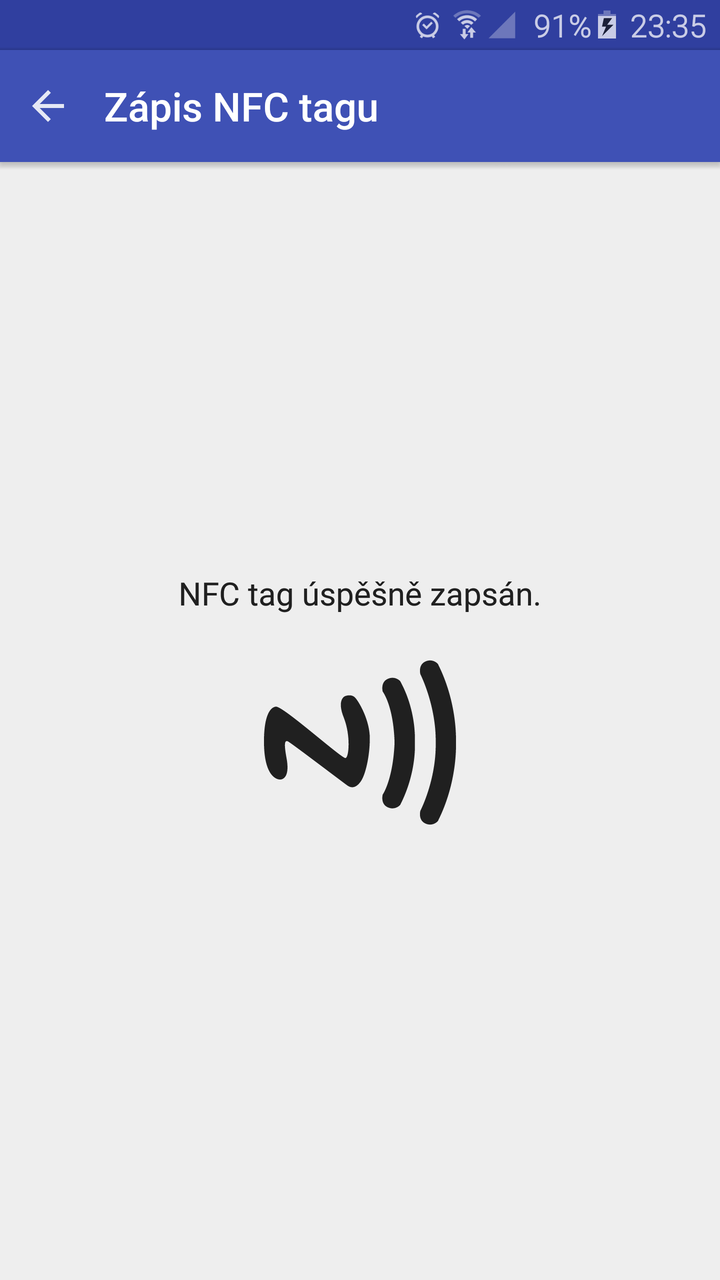
\includegraphics[scale=0.14]{img/screen/zapisdonfc.png}
            \caption{Zapsáno do NFC tagu}
            \label{fig:nfczapsano}

       \end{minipage}
\end{figure}



\usecase{Editace cesty}{editacecesty}
\textbf{Aktéři:} Asistent

\vspace{0.1cm}
\noindent
\textbf{Hlavní scénář:} Uživatel může editovat všechny uložené informace o cestě. Přepsání editačních
polí může změnit názvy a popis nahrané cesty, podržením a přetažením miniatur fotek nebo ikon dalších údajů na mapě může změnit
jejich pozici a tudíž místo, kdy se později vyvolají. Dále může podržením přetažením měnit tvar trasy,
při klepnutí na mapu přidat další záznamy. Jakmile je uživatel s editací spokojen, klepnutím na tlačítko
uložit se údaje zapíší do databáze a následující asistence cestování bude tyto údaje používat.

\vspace{0.1cm}
\noindent
\textbf{Prekondice:} Cesta je uložena.

\vspace{0.1cm}
\noindent
\textbf{Spouštěč:} Uživatel klepne na tlačítko editovat v detailu cesty.

\vspace{0.1cm}
\noindent
\textbf{Rozšíření:}
\begin{itemize}
  \item \nameref{pridanifotky}
  \item \nameref{pridaninahravky}
  \item \nameref{pridanipoznamky}
  \item \nameref{pridanizmenyprostredku}
    \item \nameref{odebranifotky}
    \item \nameref{odebraninahravky}
    \item \nameref{odebranipoznamky}
    \item \nameref{odebranizmenyprostredku}
\end{itemize}

\usecase{Přidání fotky}{pridanifotky}
\textbf{Aktéři:} Asistent

\vspace{0.1cm}
\noindent
\textbf{Hlavní scénář:} Spustí se fotoaparát zařízení a uživatel může začít fotit. Jakmile pořídí
fotografii, zobrazí se v aplikace okno pro zadání názvu fotky s dotazem pro uložení. Uživatel zadá název
a klepnutím na potvrzovací tlačítko se fotka uloží mezi data aplikace a zobrazí mezi aktuálními fotografiemi
na místě polohy uživatele v době pořízení fotografie. Uložení fotky lze vidět na obrázku~\ref{fig:pridanifotky}.

\vspace{0.1cm}
\noindent
\textbf{Prekondice:} Uživatel nahrává nebo edituje cestu.

\vspace{0.1cm}
\noindent
\textbf{Spouštěč:} Uživatel klepl na tlačítko přidat fotku.

\begin{figure}[H]
\begin{minipage}{.5\textwidth}
\centering
                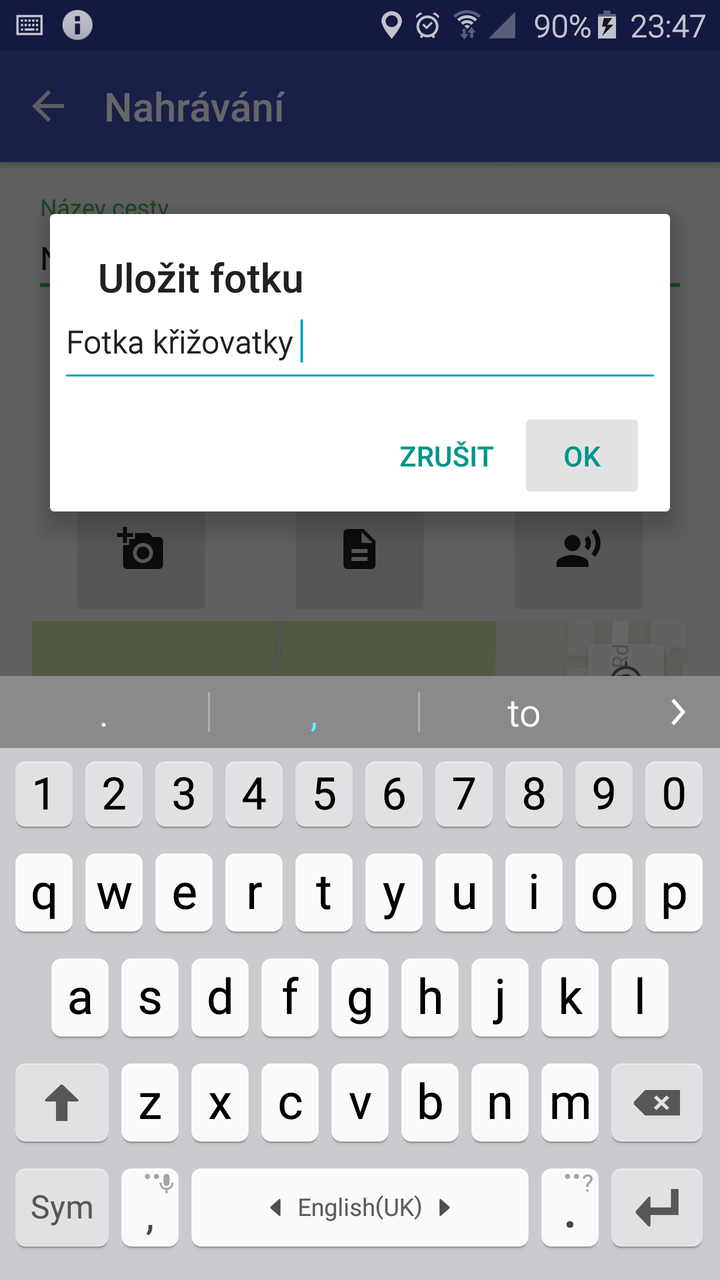
\includegraphics[scale=0.14]{img/screen/ulozenifotky.png}
        \caption{Pojmenování fotky po pořízení}
        \label{fig:pridanifotky}
\end{minipage}
\begin{minipage}{.5\textwidth}
     \centering
                     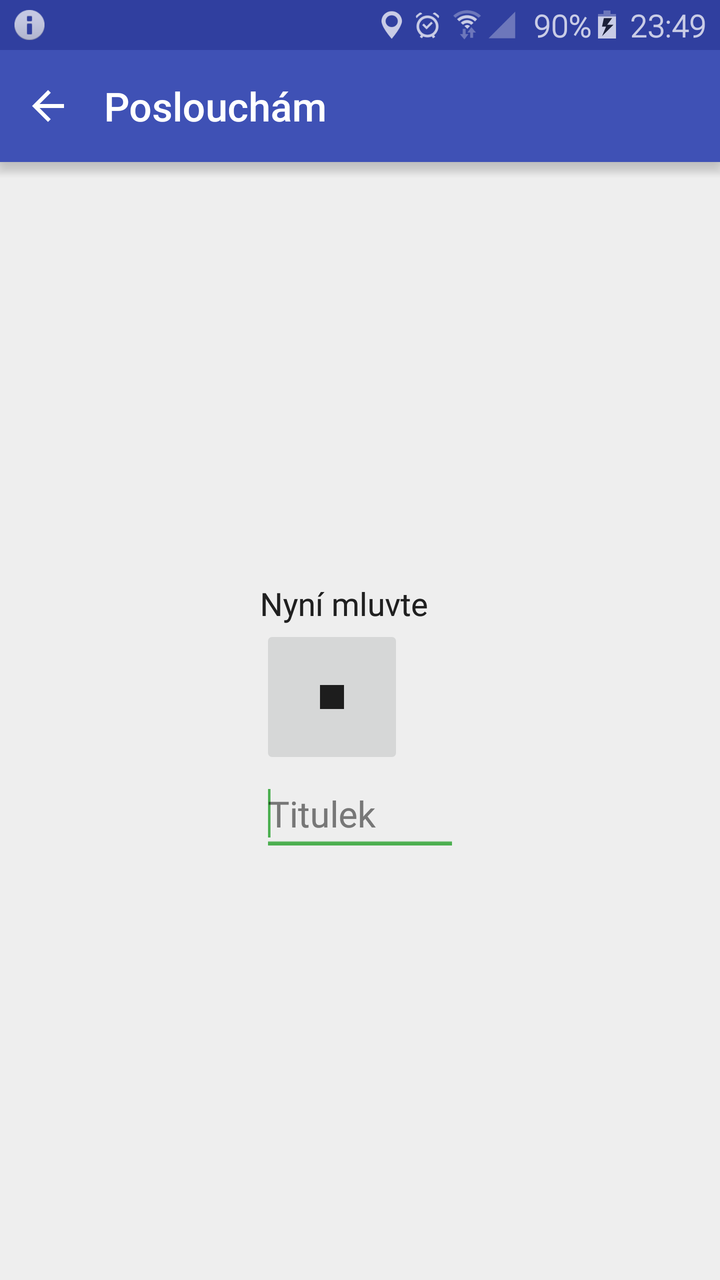
\includegraphics[scale=0.14]{img/screen/nahravaninahravky.png}
             \caption{Přidání zvukové nahrávky}
             \label{fig:pridaninahravky}

       \end{minipage}
\end{figure}

\usecase{Přidání zvukové nahrávky}{pridaninahravky}
\textbf{Aktéři:} Asistent

\vspace{0.1cm}
\noindent
\textbf{Hlavní scénář:} Uživateli se zobrazí obrazovka s textem mluvte a zvuk se zaznamenává.
Když je uživatel hotov, klepne na tlačítko stop a může nahrávce přidat název, který se bude později zobrazovat.
Poté tlačítkem nahrávku uloží mezi data aplikace s přiřazenou aktuální polohou uživatele.
Zobrazení nahrávání lze vidět na obrázku~\ref{fig:pridaninahravky}.

\vspace{0.1cm}
\noindent
\textbf{Prekondice:} Uživatel nahrává nebo edituje cestu.

\vspace{0.1cm}
\noindent
\textbf{Spouštěč:} Uživatel klepl na tlačítko přidat nahrávku.




\usecase{Přidání poznámky}{pridanipoznamky}
\textbf{Aktéři:} Asistent

\vspace{0.1cm}
\noindent
\textbf{Hlavní scénář:} Uživateli se zobrazí okno s textovým vstupem a vysune se klávesnice. Uživatel
zadá textovou poznámku a po klepnutí na potvrzovací tlačítko se poznámka uloží s asociací k aktuální poloze
uživatele. Okno přidávání poznámky lze vidět na obrázku~\ref{fig:pridanipoznamky}.

\vspace{0.1cm}
\noindent
\textbf{Prekondice:} Uživatel nahrává nebo edituje cestu.

\vspace{0.1cm}
\noindent
\textbf{Spouštěč:} Uživatel klepl na tlačítko přidat poznámku.

\begin{figure}[H]
\begin{minipage}{.5\textwidth}
\centering
                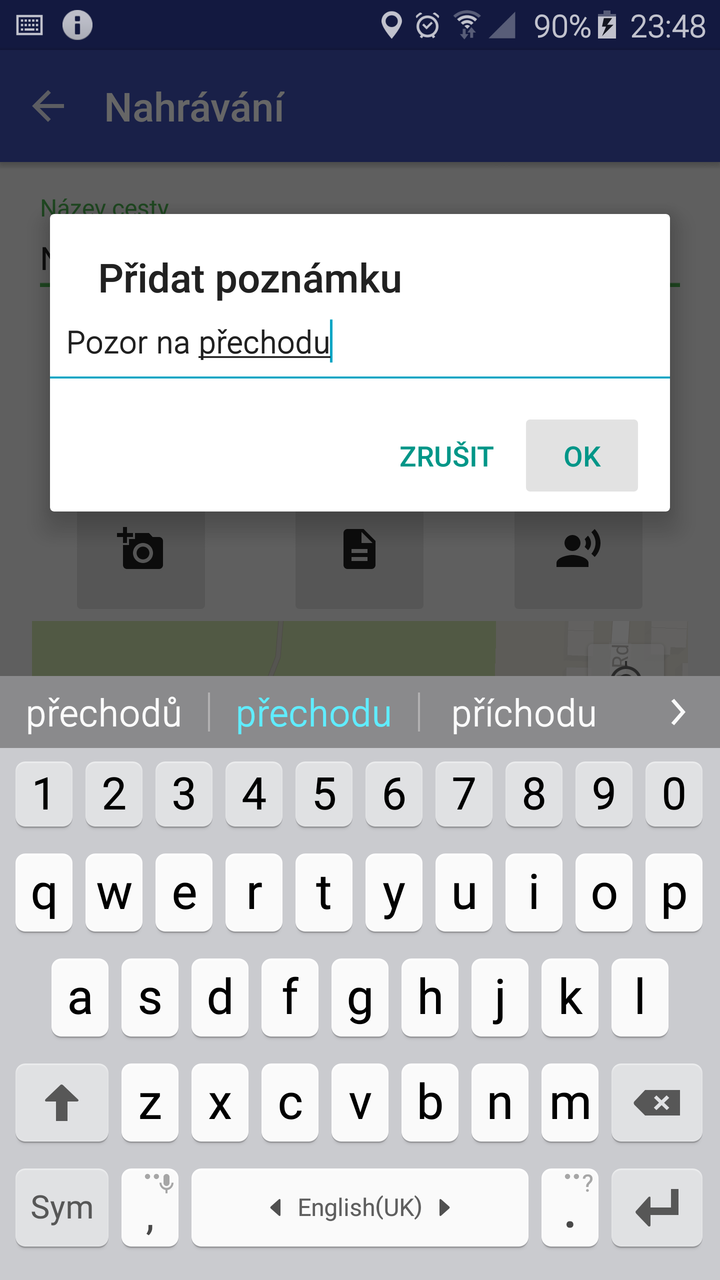
\includegraphics[scale=0.14]{img/screen/pridanipoznamky.png}
        \caption{Přidání poznámky}
        \label{fig:pridanipoznamky}
\end{minipage}
\begin{minipage}{.5\textwidth}
  \centering
                  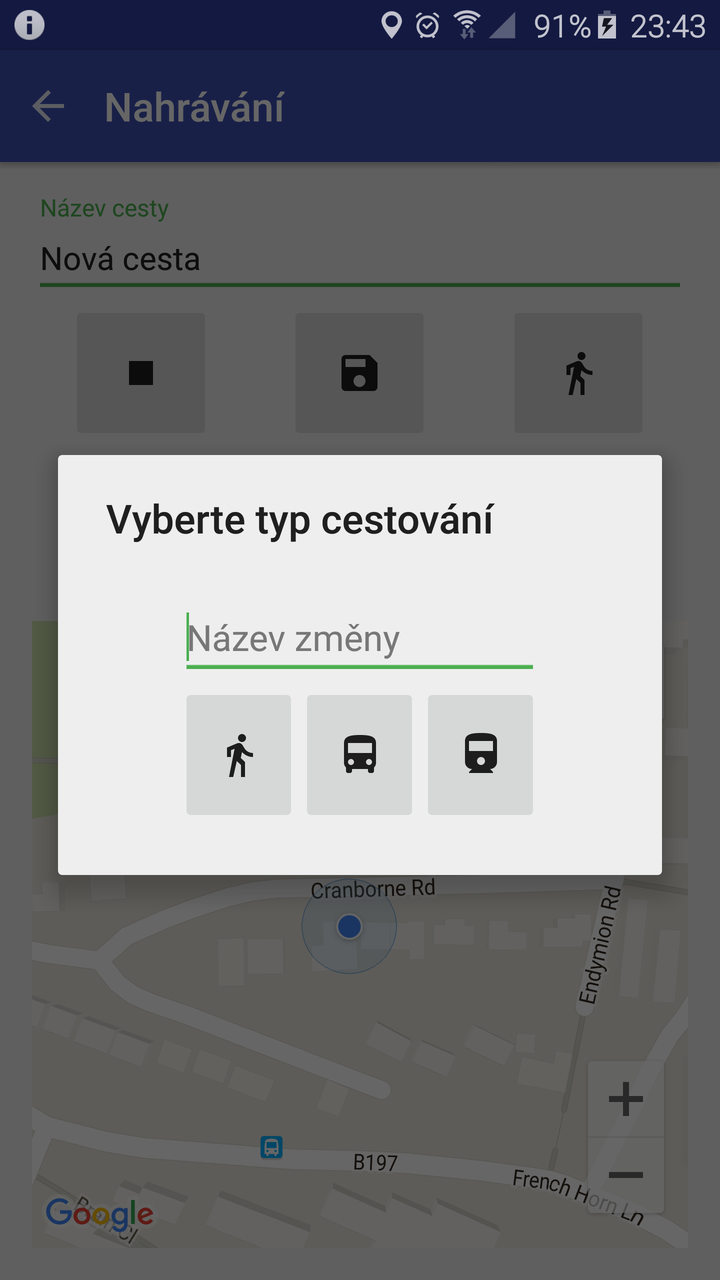
\includegraphics[scale=0.14]{img/screen/zmenaprostredku.png}
          \caption{Změna dopravního prostředku}
          \label{fig:pridanizmenyprostredku}

       \end{minipage}
\end{figure}

\usecase{Přidání změny dopravního prostředku}{pridanizmenyprostredku}
\textbf{Aktéři:} Asistent


\vspace{0.1cm}
\noindent
\textbf{Hlavní scénář:} Zobrazí se okno se nabídkou tlačítek s obrázkem dopravního prostředku.
Uživatel může zároveň přidat ke změně dopravního prostředku popisný text. Po kliknutí na
tlačítko s dopravním prostředkem se změna dopravního prostředku uloží s asociovanou aktuální polohou
uživatele. Okno změny dopravního prostředku lze vidět na obrázku~\ref{fig:pridanizmenyprostredku}.

\vspace{0.1cm}
\noindent
\textbf{Prekondice:} Uživatel nahrává nebo edituje cestu.

\vspace{0.1cm}
\noindent
\textbf{Spouštěč:} Uživatel klepl na tlačítko s aktuálním dopravním prostředkem.




\usecase{Nahrávání cesty}{nahravanicesty}
\textbf{Aktéři:} Asistent

\vspace{0.1cm}
\noindent
\textbf{Hlavní scénář:} Uživateli se zobrazí nahrávací okno, kde může vidět svou aktuální pozici
a po klepnutí na tlačítko nahrávat začne aplikace sbírat data o poloze a umožní mu přidávat další data
k právě nahrávané pozici. V notifikační liště se objeví upozornění o tom, že aplikace právě nahrává.
Uživatel může v tu chvíli odejít z aplikace, případně navštívit její jiné obrazovky a poté se do nahrávání vrátit,
aniž by ztratil právě nahrávaná data. Stejně tak po opuštění aplikace při nahrávání se do ní může vrátit
klepnutím na zobrazenou notifikaci.

Na mapě vidí uživatel dosud nahranou a uloženou cestu a případné přidané data.
Klepnutím na tlačítko uložit se aktuálně nahraní data a média uloží, případně aktualizují.
Pokud uživatel dokončil nahrávání cesty, klepne na tlačítko uložit a poté tlačítkem stop zastaví nahrávání,
notifikace zmizí a cesta je v seznamu cest připraveno pro spuštění asistence, případně následnou editaci.
Pokud uživatel ukončí nahrávání bez uložení, je na toto upozorněn a při potvrzení ukončení jsou nahraná data
smazána. Obrazovku nahrávání můžeme vidět na obrázku~\ref{fig:nahravanicestyicon} a zobrazenou notifikaci
na obrázku~\ref{fig:notifikacenahravanicesty}.

\vspace{0.1cm}
\noindent
\textbf{Prekondice:} Uživatel má v telefonu povolené získávání polohy pomocí GPS.

\vspace{0.1cm}
\noindent
\textbf{Spouštěč:} Uživatel klepne na tlačítko nahrávat v seznamu nahraných cest.

\vspace{0.1cm}
\noindent
\textbf{Rozšíření:}
\begin{itemize}
  \item \nameref{pridanifotky}
  \item \nameref{pridaninahravky}
  \item \nameref{pridanipoznamky}
  \item \nameref{pridanizmenyprostredku}
  \item \nameref{odebranifotky}
  \item \nameref{odebraninahravky}
  \item \nameref{odebranipoznamky}
  \item \nameref{odebranizmenyprostredku}
\end{itemize}

\begin{figure}[H]
\begin{minipage}{.5\textwidth}


        \centering
                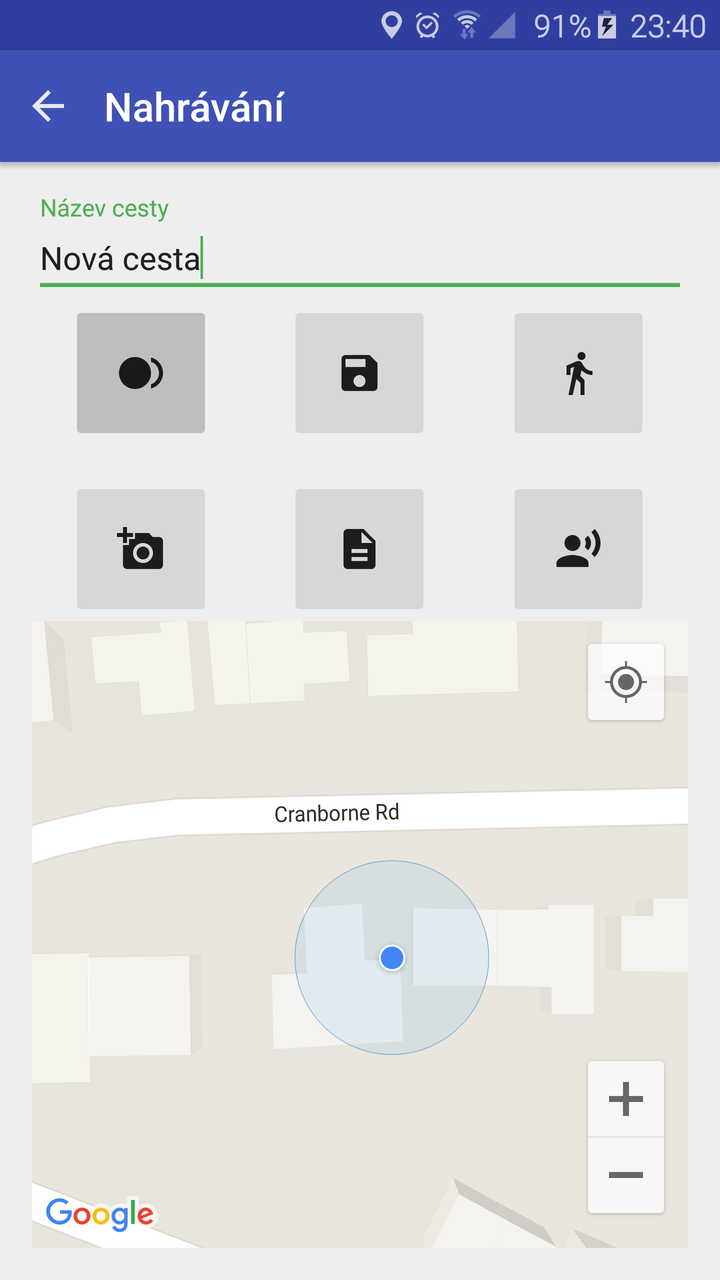
\includegraphics[scale=0.14]{img/screen/nahravani.png}
        \caption{Nahrávání cesty}
        \label{fig:nahravanicestyicon}
\end{minipage}
\begin{minipage}{.5\textwidth}
  \centering
                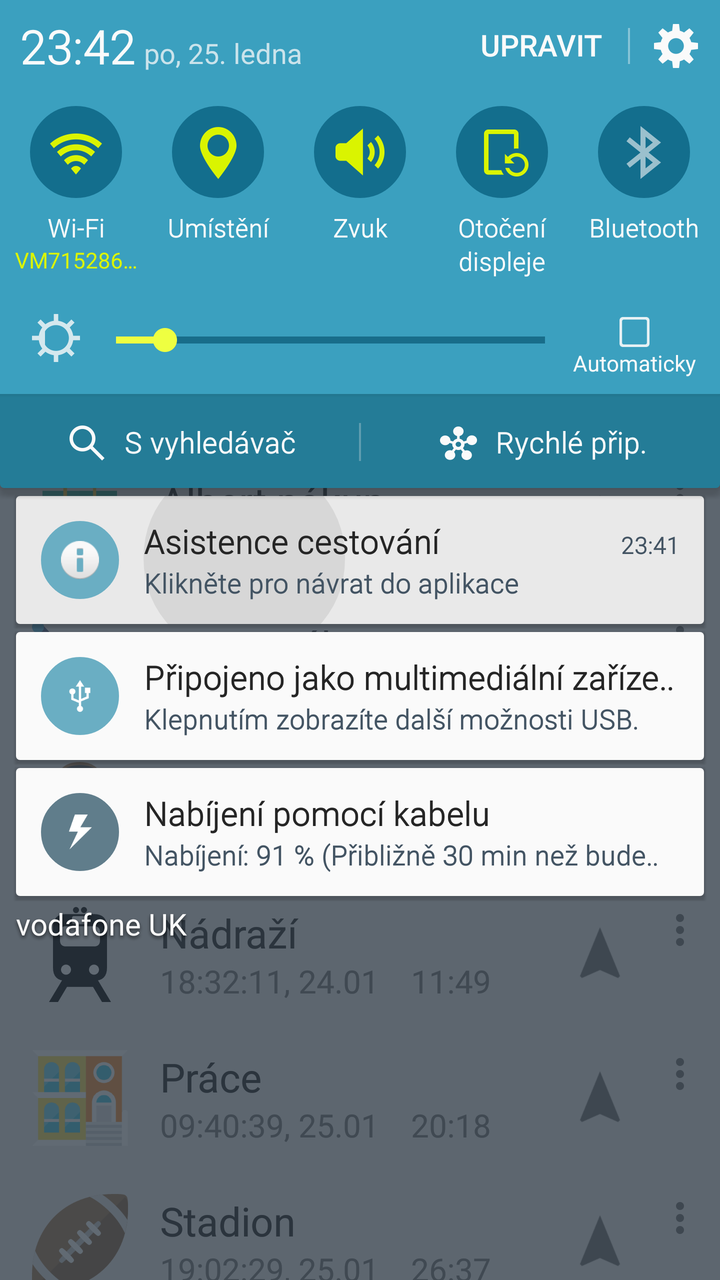
\includegraphics[scale=0.14]{img/screen/notifikace.png}
        \caption{Zobrazená notifikace}
        \label{fig:notifikacenahravanicesty}

       \end{minipage}
\end{figure}


\usecase{Odebrání fotky}{odebranifotky}
\textbf{Aktéři:} Asistent

\vspace{0.1cm}
\noindent
\textbf{Hlavní scénář:} Uživateli se zobrazí okno s dotazem zda chce fotku odebrat. Po klepnutí na
potvrzovací tlačítko je fotka smazána z úložiště a odstraněna její miniatura z aktuální cesty.

\vspace{0.1cm}
\noindent
\textbf{Prekondice:} Uživatel nahrává nebo edituje cestu a má uloženou fotografii.

\vspace{0.1cm}
\noindent
\textbf{Spouštěč:} Uživatel podrží prst na miniatuře fotografie a vybere možnost smazat.



\usecase{Odebrání zvukové nahrávky}{odebraninahravky}
\textbf{Aktéři:} Asistent

\vspace{0.1cm}
\noindent
\textbf{Hlavní scénář:} Uživateli se zobrazí dotaz zda chce nahrávku opravdu smazat, po potvrzení
se uložená nahrávka odstraní a zmizí její ikona.

\vspace{0.1cm}
\noindent
\textbf{Prekondice:} Uživatel nahrává nebo edituje cestu a má uloženou nahrávku.

\vspace{0.1cm}
\noindent
\textbf{Spouštěč:} Uživatel podrží prst na ikoně nahrávky a vybere možnost smazat.



\usecase{Odebrání poznámky}{odebranipoznamky}
\textbf{Aktéři:} Asistent

\vspace{0.1cm}
\noindent
\textbf{Hlavní scénář:} Uživateli se zobrazí okno s dotazem na smazání poznámky. Po potvrzení se
nahrávka smaže a zmizí ikona indikující nahrávku.

\vspace{0.1cm}
\noindent
\textbf{Prekondice:} Uživatel nahrává nebo edituje cestu a má uloženou poznámku.

\vspace{0.1cm}
\noindent
\textbf{Spouštěč:} Uživatel podrží prst na ikoně poznámky a vybere možnost smazat.


\usecase{Odebrání změny dopravního prostředku}{odebranizmenyprostredku}
\textbf{Aktéři:} Asistent

\vspace{0.1cm}
\noindent
\textbf{Hlavní scénář:} Uživateli se zobrazí okno s dotazem na smazání změny dopravního prostředku.
Po potvrzení se nahrávka smaže a zmizí ikona indikující nahrávku. Zobrazené nastavení údajů
lze vidět na obrázku~\ref{fig:nastaveniudaju}.

\vspace{0.1cm}
\noindent
\textbf{Prekondice:} Uživatel nahrává nebo edituje cestu a má uloženou změnu dopravního prostředku.

\vspace{0.1cm}
\noindent
\textbf{Spouštěč:} Uživatel podrží prst na ikoně změny dopravního prostředku a vybere možnost smazat.


\usecase{Nastavení údajů asistenta}{nastaveniudaju}
\textbf{Aktéři:} Asistent

\vspace{0.1cm}
\noindent
\textbf{Hlavní scénář:} Uživateli se zobrazí obrazovka s nastavením údajů, kde může vyplnit své údaje.

\vspace{0.1cm}
\noindent
\textbf{Spouštěč:} Uživatel klepl na tlačítko nastavení.

\vspace{0.1cm}
\noindent
\textbf{Rozšíření:}
\begin{itemize}
  \item \nameref{nastavenicisla}
  \item \nameref{nastaveniemailu}
\end{itemize}

\begin{figure}[H]
\begin{minipage}{.5\textwidth}
\centering
                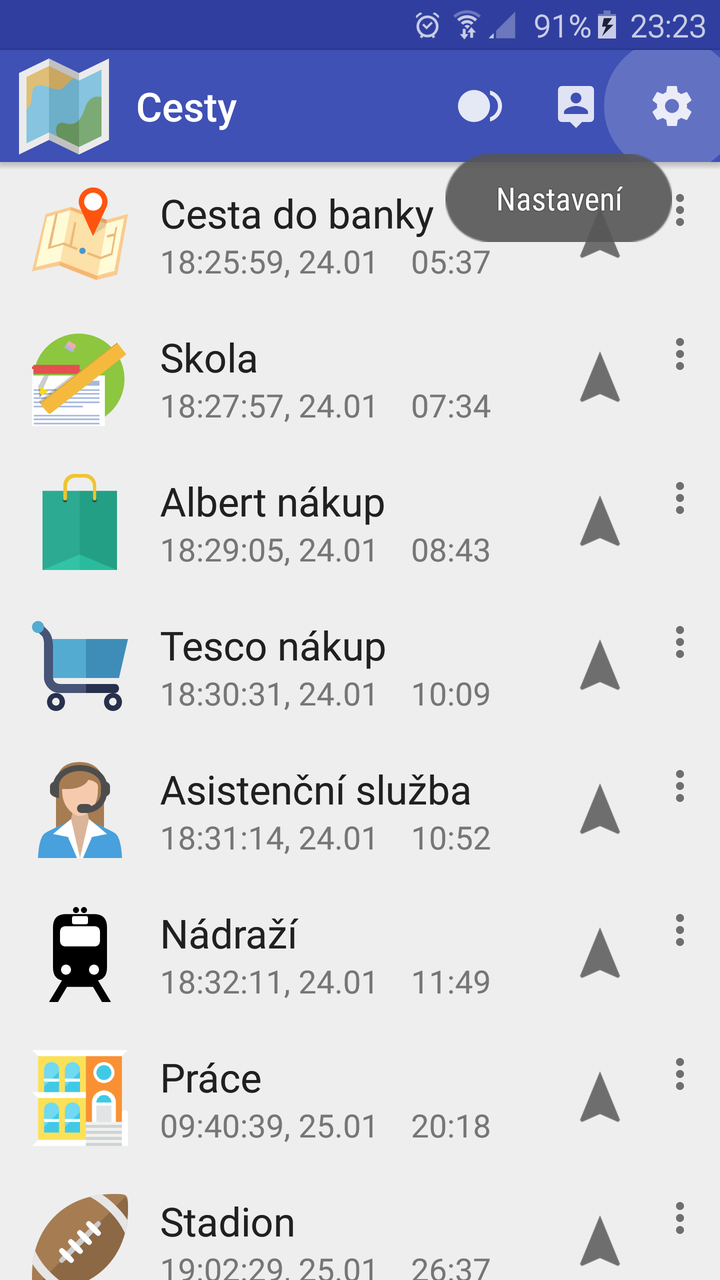
\includegraphics[scale=0.14]{img/screen/nastaveni.png}
        \caption{Spuštění nastavení údajů}
        \label{fig:nastaveniudaju}
\end{minipage}
\begin{minipage}{.5\textwidth}
\centering
                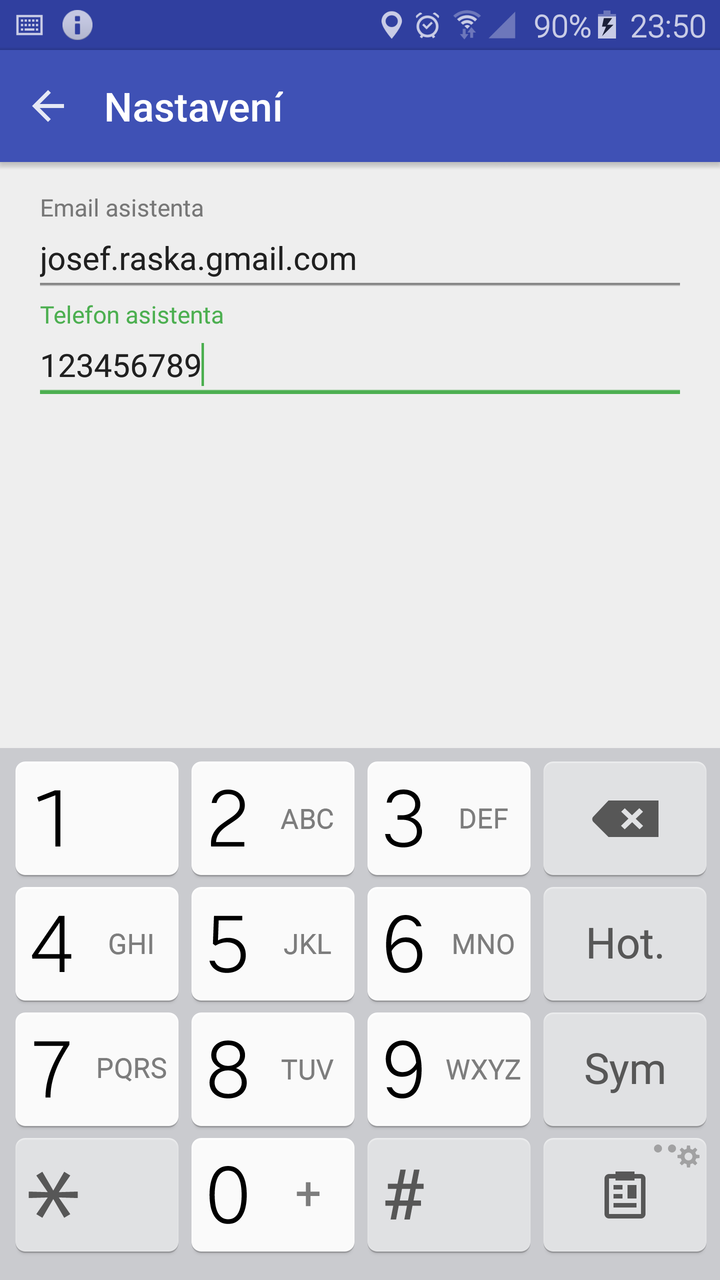
\includegraphics[scale=0.14]{img/screen/nastaveniasistent.png}
        \caption{Nastavení telefonního čísla}
        \label{fig:nastavenicisla}
    \end{minipage}
\end{figure}

\usecase{Nastavení telefonního čísla asistenta}{nastavenicisla}
\textbf{Aktéři:} Asistent

\vspace{0.1cm}
\noindent
\textbf{Hlavní scénář:} Editovatelné pole pro telefonní číslo se zvýrazní a vysune se numerická klávesnice.
Uživatel zadá své telefonní číslo, které se automaticky formátuje do přívětivějšího formátu. Po ukončení
editace je telefonní číslo automaticky uloženo. Pokud telefonní číslo neodpovídá formátu telefonních čísel
v České republice, uživatel je na toto upozorněn a je vyzván k úpravě vstupu. Zadávání telefonního čísla
vidíme na obrázku~\ref{fig:nastavenicisla}.

\vspace{0.1cm}
\noindent
\textbf{Spouštěč:} Uživatel klepl na editační pole s telefonním číslem asistenta.

\usecase{Nastavení emailu asistenta}{nastaveniemailu}
\textbf{Aktéři:} Asistent

\vspace{0.1cm}
\noindent
\textbf{Hlavní scénář:} Editovatelné pole pro emailovou adresu se zvýrazní a vysune se klávesnice.
Uživatel zadá svou emailovou adresu. Po ukončení editace je emailová adresa automaticky uložena.
Pokud emailová adresa neodpovídá správnému formátu emailové adresy, uživatel je na toto upozorněn
a vyzván k úpravě vstupu.

\vspace{0.1cm}
\noindent
\textbf{Spouštěč:} Uživatel klepl na editovatelné pole emailové adresy.


\usecase{Nastavení zamčení editace}{nastavenizamceni}
\textbf{Aktéři:} Asistent

\vspace{0.1cm}
\noindent
\textbf{Hlavní scénář:} Uživateli se zobrazí editovatelné pole, kde může zadat heslo pro zamčení editace
obsahu aplikace. Pokud toto heslo nezadá, aplikace bude stále v módu editace a uložená data bude možné upravit.
Uživatel zadá heslo, to bude uloženo a bude nyní vyžadováno pro zpřístupnění úprav cest, případně nastavení.

\vspace{0.1cm}
\noindent
\textbf{Spouštěč:} Uživatel klepl na tlačítko nastavení zamčení.

\usecase{Nastavení zálohování}{nastavenizalohovani}
\textbf{Aktéři:} Asistent

\vspace{0.1cm}
\noindent
\textbf{Hlavní scénář:} Uživateli se zobrazí výběr z listu zda chce zálohovat manuálně, jednou za den, týden
nebo za měsíc. Uživatel vybere jednu z možností a podle výběru se naplánují příslušné akce.

\vspace{0.1cm}
\noindent
\textbf{Prekondice:} Uživatel má na zařízení nastaven účet umožňující zálohování.

\vspace{0.1cm}
\noindent
\textbf{Spouštěč:} Uživatel klepl na tlačítko nastavení zálohování.


















\subsection{Use casy uživatele Klient}
Pro klienta jsou určeny více intuitivní a nenáročné operace vyžadující co nejméně aktivních
kroků z klientovi strany. Aplikace by měla na základě polohy a dalších údajů sama rozpoznat,
co má v danou chvíli udělat. Use casy klienta a jejich vztahy lze vidět na obrázku~\ref{fig:UseCasesClient}.

\begin{figure}[H]
        \centering
                \includegraphics[scale=0.2]{img/UseCasesClient.png}
        \caption{Diagram use casů uživatele klient}
        \label{fig:UseCasesClient}
\end{figure}


\usecase{Prohlížení seznamu nahraných cest}{prohlizeniklient}
\textbf{Aktéři:} Klient

\vspace{0.1cm}
\noindent
\textbf{Hlavní scénář:} Na úvodní obrazovce jsou pod sebou vyobrazeny všechny cesty, pro které může
uživateli aplikace poskytnout asistenci. Uživatel si prohlíží cesty, které mají zobrazeny pouze
základní informace a jsou označeny vybraným obrázkem pro snazší orientaci. Uživatel si poklepnutím
na řádek cesty může dostat na její detail případně rychlými akcemi spustí navigaci.

\vspace{0.1cm}
\noindent
\textbf{Spouštěč:} Uživatel klepne na ikonu aplikace v telefonu.

\vspace{0.1cm}
\noindent
\textbf{Rozšíření:}
\begin{itemize}
  \item \nameref{detailklient}
  \item \nameref{asistence}
\end{itemize}

\usecase{Detail nahrané cesty}{detailklient}
\textbf{Aktéři:} Klient

\vspace{0.1cm}
\noindent
\textbf{Hlavní scénář:} Klientovi se zobrazí obrazovka se všemi údaji, které mu mají na cestě pomoci.
Fotky jsou vidět jako miniatury na místě, kde byly pořízeny, podobně nahrávky, změny dopravního prostředku
a poznámky, které jsou reprezentovány svými příslušnými jednoduchými ikonami.

\vspace{0.1cm}
\noindent
\textbf{Prekondice:} Uživatel má nahranou cestu.

\vspace{0.1cm}
\noindent
\textbf{Spouštěč:} Uživatel klepne na řádek cesty v seznamu nahraných cest.

\vspace{0.1cm}
\noindent
\textbf{Rozšíření:}
\begin{itemize}
  \item \nameref{asistence}
\end{itemize}


\usecase{Asistence cestování}{asistence}
\textbf{Aktéři:} Klient

\vspace{0.1cm}
\noindent
\textbf{Hlavní scénář:} Uživateli se zobrazí jednoduchá mapka s vyznačenou cestou, kterou má absolvovat.
Zobrazí se mu všechny dostupné informace jako čas do cíle, doporučený směr, nejbližší nahrané fotky,
nahrávky nebo poznámky. Zkontroluje se podle uložených statistik, zda bude uživateli stačit baterie
k absolvování cesty a pokud ne, bude na to upozorněn.
Aplikace využívá klientovu polohu pro zobrazení relevantních nahraných informací
a snaží se mu napovídat následující směr pomocí zobrazené šipky. Jak se klient pohybuje, aplikace mu
poskytuje nahraný obsah asistentem, který by mu měl pomoci v danou chvíli se lépe zorientovat.
Obrazovku asistence cestování lze vidět na obrázku~\ref{fig:asistence}.

\vspace{0.1cm}
\noindent
\textbf{Prekondice:} Klient má nahranou cestu a spustil asistenci cestování po této cestě.

\vspace{0.1cm}
\noindent
\textbf{Spouštěč:} Klient klepl na obrázek navigovat.

\vspace{0.1cm}
\noindent
\textbf{Rozšíření:}
\begin{itemize}
  \item \nameref{zobrazenifotky}
  \item \nameref{prehraninahravky}
  \item \nameref{zobrazenipoznamky}
  \item \nameref{upozorneniprostredek}
  \item \nameref{analyzabaterie}
  \item \nameref{zobrazenismeru}
  \item \nameref{upozorneninespravnysmer}
\end{itemize}


\begin{figure}[H]
\begin{minipage}{.5\textwidth}
\centering
                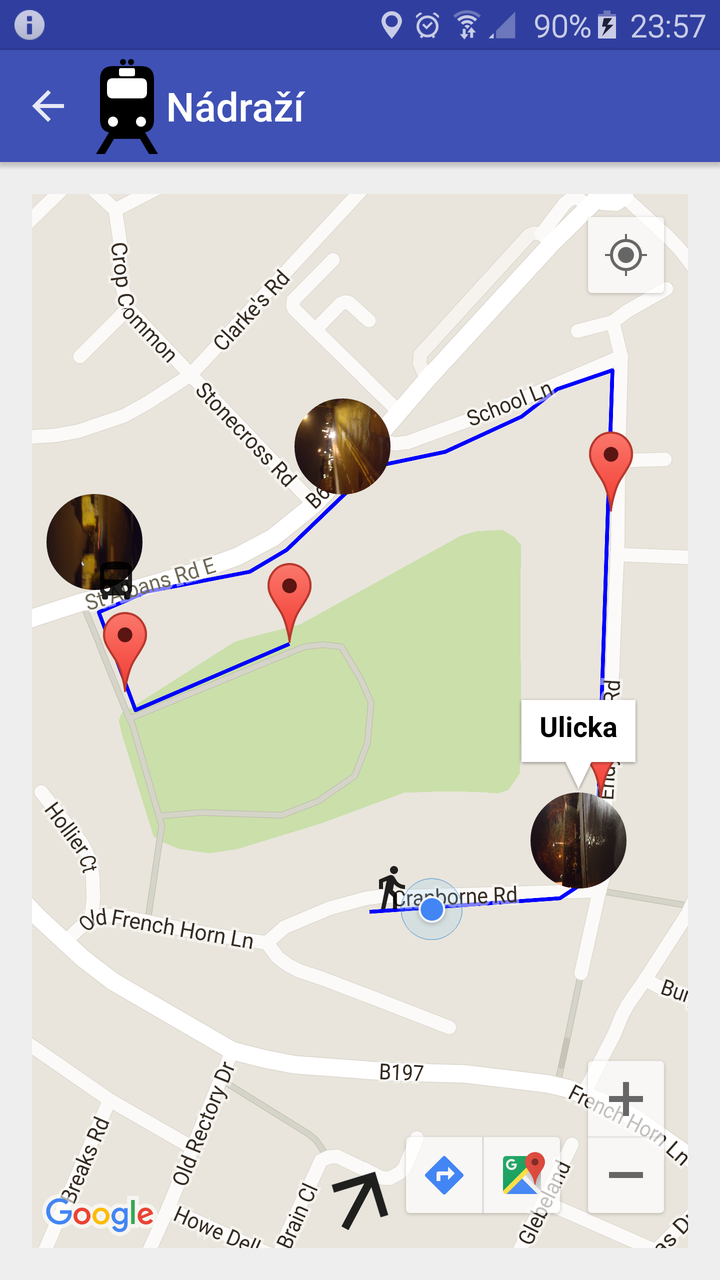
\includegraphics[scale=0.14]{img/screen/asistencecestovani.png}
        \caption{Asistence cestování}
        \label{fig:asistence}
\end{minipage}
\begin{minipage}{.5\textwidth}
\centering
                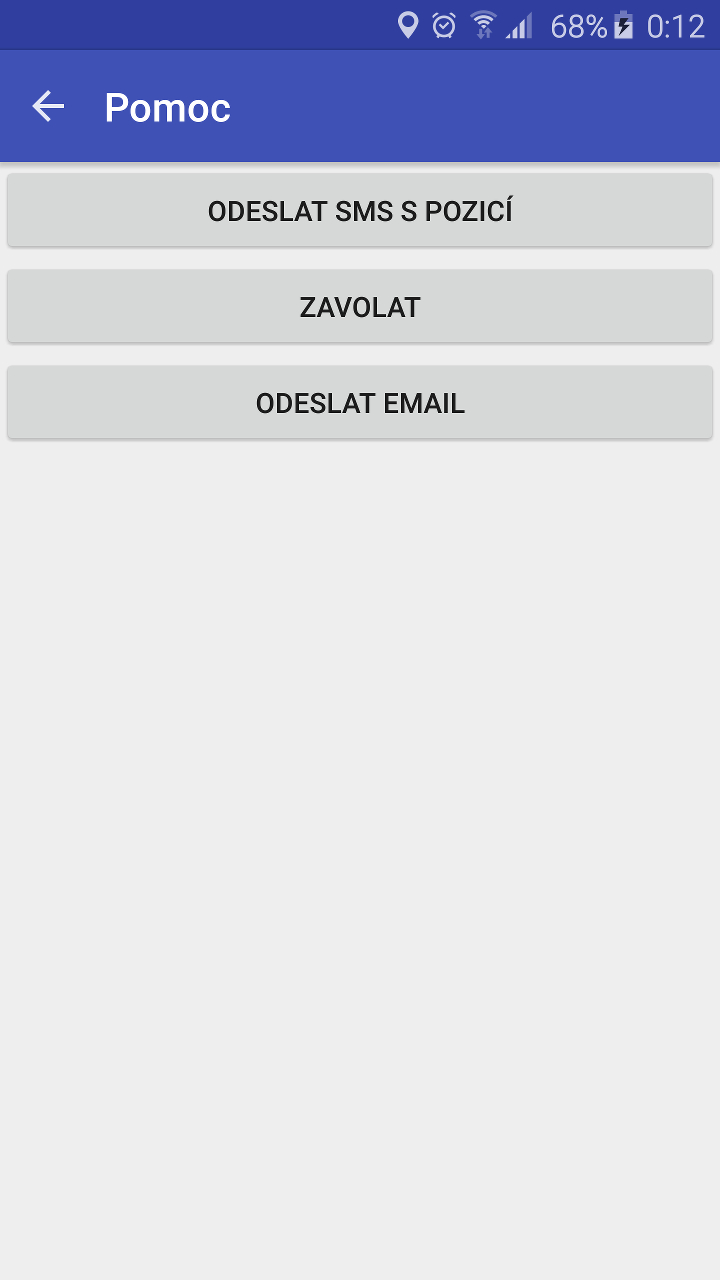
\includegraphics[scale=0.14]{img/screen/volanipomoc.jpg}
        \caption{Obrazovka pomoci}
        \label{fig:pomoc}
    \end{minipage}
\end{figure}



\usecase{Zobrazení fotografie}{zobrazenifotky}
\textbf{Aktéři:} Klient

\vspace{0.1cm}
\noindent
\textbf{Hlavní scénář:} Uživatel se přiblíží k místu pořízení fotografie, aplikace toto rozpozná
a upozorní uživatele na přítomnost fotky, která se zobrazí na dobu, po kterou je uživatel nablízku.
Přes spodní část fotky je zobrazen popisek, který této fotce dříve zadal asistent.

\vspace{0.1cm}
\noindent
\textbf{Prekondice:} Uživatel má k dané cestě uloženou fotku.

\vspace{0.1cm}
\noindent
\textbf{Spouštěč:} Uživatel se přiblíží místu pořízení fotky nebo klepne na miniaturu fotky.


\usecase{Přehrání uložené zvukové nahrávky}{prehraninahravky}
\textbf{Aktéři:} Klient

\vspace{0.1cm}
\noindent
\textbf{Hlavní scénář:} Uživatel se se zapnutou asistencí cestování přiblíží místu,
kde byla dříve za pomoci asistenta pořízena zvuková nahrávka. Uložená nahrávka se načte
a začne se uživateli přehrávat. Zároveň se zobrazí popis nahrávky a tlačítko umožňující
nahrávku přehrát znovu.

\vspace{0.1cm}
\noindent
\textbf{Prekondice:} Uživatel má k dané cestě uloženou zvukovou nahrávku.

\vspace{0.1cm}
\noindent
\textbf{Spouštěč:} Uživatel se přiblíží k místu pořízení nahrávky nebo klepne na ikonu nahrávky.

\usecase{Zobrazení uložené poznámky}{zobrazenipoznamky}
\textbf{Aktéři:} Klient

\vspace{0.1cm}
\noindent
\textbf{Hlavní scénář:} Uživatel je při přiblížení se místu poznámky upozorněn a poznámka se zobrazí.

\vspace{0.1cm}
\noindent
\textbf{Prekondice:} Uživatel má k dané cestě uloženou poznámku.

\vspace{0.1cm}
\noindent
\textbf{Spouštěč:} Uživatel se přiblíží k místu pořízení poznámky nebo klepne na ikonu poznámky.

\usecase{Upozornění na změnu dopravního prostředku}{upozorneniprostredek}
\textbf{Aktéři:} Klient

\vspace{0.1cm}
\noindent
\textbf{Hlavní scénář:} Uživateli je při přiblížení ke změně dopravního prostředku upozorněn,
zobrazí se mu obrázek dopravního prostředku, do kterého má nastoupit nebo naopak vystoupit spolu
s textem, který byl při nahrávání cesty zadán.

\vspace{0.1cm}
\noindent
\textbf{Prekondice:} Uživatel má uloženo upozornění na změnu dopravního prostředku.

\vspace{0.1cm}
\noindent
\textbf{Spouštěč:} Uživatel se přiblíží k místu změny dopravního prostředku.



\usecase{Analýza spotřeby baterie}{analyzabaterie}
\textbf{Aktéři:} Klient

\vspace{0.1cm}
\noindent
\textbf{Hlavní scénář:} Během cestování se ukládají průběžně data o spotřebě beterie a délce trvání
cesty. Data jsou poté spolu s předchozími záznamy statisticky analyzována a je odhadována a upřesňována
očekávaná výdrž baterie během navigace. Na základě těchto analýz může být uživatel poté upozorněn na
nebezpečí vybití baterie v terénu.

\vspace{0.1cm}
\noindent
\textbf{Spouštěč:} Uživatel využívá asistence při cestování.



\usecase{Zobrazení doporučeného směru}{zobrazenismeru}
\textbf{Aktéři:} Klient

\vspace{0.1cm}
\noindent
\textbf{Hlavní scénář:} Na základě pohybu uživatele jsou data vyhodnocována a vypočítán aktuální směr uživatele.
Ten se porovná s očekávaným a uloženým směrem a podle rozdílu se zobrazí směr, kterým by se uživatel měl ideálně
vydat. Informace je zobrazena v dolní části obrazovky v podobě jednoduché šipky.

\vspace{0.1cm}
\noindent
\textbf{Prekondice:} Uživatel se pohybuje po cestě nebo chodníku.

\vspace{0.1cm}
\noindent
\textbf{Spouštěč:} Uživatel využívá asistence při cestování.


\usecase{Upozornění na nesprávný směr}{upozorneninespravnysmer}
\textbf{Aktéři:} Klient

\vspace{0.1cm}
\noindent
\textbf{Hlavní scénář:} Když se uživatel nepohybuje dle očekávané trasy, aplikace může vyhodnotit
tento pohyb jako nesprávný. V takovém případě začne uživatele upozorňovat a pokud směr nezmění nebo
neklepne na tlačítko známý směr, bude s upozorňováním pokračovat a nabízet směr správný.

\vspace{0.1cm}
\noindent
\textbf{Spouštěč:} Uživatel se během asistence cestování určitou dobu pohybuje jiným, než očekávaným směrem.


\usecase{Spuštění asistence cestování po přiložení NFC tagy k telefonu}{prilozeninfc}
\textbf{Aktéři:} Klient

\vspace{0.1cm}
\noindent
\textbf{Hlavní scénář:} Klient přiloží telefon k nálepce, kartě nebo čemukoliv jinému, co bylo použito
jako NFC tag a obsahuje informace o cestě. Tato informace se přečte a spustí se aplikace se zapnutou
asistencí cestování na cestu zapsanou na tagu.

\vspace{0.1cm}
\noindent
\textbf{Prekondice:} Klient má k dispozici NFC tag, na který byla dříve zapsána informace o cestě.

\vspace{0.1cm}
\noindent
\textbf{Spouštěč:} Klient přiloží telefon k NFC tagu.

\vspace{0.1cm}
\noindent
\textbf{Rozšíření:}
\begin{itemize}
  \item \nameref{pridanifotky}
\end{itemize}

\usecase{Vyvolání obrazovky pomoci}{pomoc}
\textbf{Aktéři:} Klient

\vspace{0.1cm}
\noindent
\textbf{Hlavní scénář:} Uživateli se zobrazí obrazovka s volbami rychlých akcí,
které kontaktují jeho asistenta. Obrazovka pomoci je na obrázku~\ref{fig:pomoc}.

\vspace{0.1cm}
\noindent
\textbf{Prekondice:} V zařízení jsou uloženy kontaktní údaje asistenta.

\vspace{0.1cm}
\noindent
\textbf{Spouštěč:} Uživatel klepne na obrázek pomoc v aplikaci.

\vspace{0.1cm}
\noindent
\textbf{Rozšíření:}
\begin{itemize}
  \item \nameref{pomocvolani}
  \item \nameref{pomocsms}
  \item \nameref{pomocemail}
\end{itemize}



\usecase{Volání asistentovi}{pomocvolani}
\textbf{Aktéři:} Klient, Asistent

\vspace{0.1cm}
\noindent
\textbf{Hlavní scénář:} Uživateli se zobrazí obrazovka, kde vidí vytáčení čísla na svého asistenta.
Hovor se poté uskuteční.

\vspace{0.1cm}
\noindent
\textbf{Prekondice:} V aplikaci je uloženo telefonní číslo asistenta.

\vspace{0.1cm}
\noindent
\textbf{Spouštěč:} Uživatel klepne na číslo asistenta.

\usecase{Poslání SMS zprávy s aktuální polohou}{pomocsms}
\textbf{Aktéři:} Klient, Asistent

\vspace{0.1cm}
\noindent
\textbf{Hlavní scénář:} Uživateli se zobrazí potvrzení o odeslání SMS zprávy a její znění.
Asistentovi se zobrazí zpráva, ve které je také odkaz na mapu s GPS polohou klienta v době odesílání zprávy.

\vspace{0.1cm}
\noindent
\textbf{Prekondice:} V aplikaci je uloženo telefonní číslo asistenta.

\vspace{0.1cm}
\noindent
\textbf{Spouštěč:} Uživatel klepne na tlačítko poslat SMS.


\usecase{Poslání emailu s aktuální polohou}{pomocemail}
\textbf{Aktéři:} Klient, Asistent

\vspace{0.1cm}
\noindent
\textbf{Hlavní scénář:} Klientovi se otevře emailová aplikace s nachystanou zprávou a adresou asistenta
a klient klepne odeslat. Asistentovi přijde email s žádostí o pomoc a odkazem na mapu s GPS polohou
klienta v době odeslání emailu.

\vspace{0.1cm}
\noindent
\textbf{Prekondice:} V aplikaci je uložena emailová adresa asistenta.

\vspace{0.1cm}
\noindent
\textbf{Spouštěč:} Uživatel klepne na tlačítko odeslat email.

\subsection{Grafický návrh}
Cílem návrhu bylo používat v aplikaci konzistentní rozhraní a také jednoduchost všech uživatelských
prvků pro snadné pochopení pro uživatele se specifickými nároky. Většina uživatelských prvků je tak
realizována jako velká tlačítka, která při podržení prstu na prvku zobrazí jeho textový popis.
Jako hlavní směr návrhu uživatelského rozhraní byl zvolen Material design, neboť se jedná o aktuální
doporučení pro mobilní aplikace a je v něm kladen velký důrazná jednoduchost a konzistenci,
tedy naše požadavky. Velkou část této specifikace za nás řeší námi používaná knihovna Android Support,
popsaná v sekci \ref{androidsupport}.

\subsubsection{Material design}
Úplnou specifikaci Material designu, vydanou poprvé v roce 2015 lze nalézt v \cite{materialdesign}.
Jedná se o detailní popis všech
grafických prvků uživatelského rozhraní, které by měl vývojář používat, jejich chování, vzhled i vzájemnou
 interakci. Jako hlavní cíl si klade vytvořit vizuální jazyk, spojující klasické principy dobrého designu
  a nových možností moderních technologií a vyvinout systém spojující zkušenost uživatele na různých
  platformách a velikostech obrazovek\cite{materialdesign}. Uživatelské rozhraní v duchu Material designu
  by mělo uživateli lépe napovídat, co který prvek dělá, pomocí animací a směru efektů přibližovat
  význam grafických komponent, případně pomocí stínů různých délek vytvářet iluzi uložení prvků
  v prostoru a jejich seřazení podle důležitosti.

  Material design používá ke specifikaci rozměrů
  stejně jako systém Android jednotku \texttt{dp}, což znamená v angličtině \uv{Device independent
  pixel} a jedná se o jednotku, která je relativní vůči skutečnému rozlišení zařízení a jejím účelem
  je zobrazení prvků uživatelského rozhraní v přibližně stejné reálné velikosti bez ohledu na skutečnou
  hustotu pixelů obrazovky, které se zařazují do tříd hustoty a podle této třídy se rozhoduje,
  kolik skutečných pixelů bude ve výsledku prvek zabírat. Tyto třídy jsou v současnosti
  \texttt{ldpi}, \texttt{hdpi}, \texttt{tvdpi}, \texttt{hdpi}, \texttt{xhdpi}, \texttt{xxhdpi} a \texttt{xxxhdpi}.
  Obdélník o šířce 100dp bude pak například v třídě rozlišení \texttt{ldpi} zabírat 75 pixelů(1dp = 0.75px),
  nicméně na zařízení ve třídě \texttt{xxxhdpi} bude mít rozměr 400 pixelů(1dp = 4px). Pro uživatelské
  prvky naší aplikace budeme vždy používat jednotku \texttt{dp}.

  Specifikace zavádí jako jednu ze svých hlavních prvků zavedení prostorové osy \textit{z} do
  definice uživatelského rozhraní a nazývá tuto vlastnost uživatelských prvků vyvýšení(elevation)\cite{materialdesign}.
  Tato vlastnost ovlivňuje nejvíce velikost stínu uživatelského prvku. Nejvyšší vyvýšení(24dp)
  mají modální dialogy, poté postranní menu(16dp) následují další komponenty, mezi nimiž jsou námi využívané
  menu(8dp), vyjíždějící upozornění "Snackbar"(6dp), případně lišta menu rychlých akcí "App bar"(4dp)\cite{materialdesign}.
  Specifikace přesně určuje chování pro každou komponentu a precizně tak vývojáře vede ke správné
  implementaci uživatelských prvků.


\subsubsection{Barvy}
  Material design také poskytuje barvy, které by měly být v naší aplikaci použity jako dominantní v hlavních
  uživatelských prvcích. Paletu barev můžeme nalézt na \url{https://www.google.com/design/spec/style/color.html}  (10.4.2016).
  Pro naší aplikaci byla vybrána jako hlavní barvy odstíny barvy indiga a zdůrazňující barvou byla zvolena zelená.
  Jako barvy textu byla vybrána čistě bíla pro nadpisy na hlavních barvách, lehce průhledná černá pro
  primární text a šedá pro sekundární text. Jako barva pozadí těla byla ponechána výchozí lehce ztmavená bílá
  barva. Popsané barvy s ukázkou můžeme vidět na obrázku \ref{fig:colorpalette}.

  \begin{figure}[H]
          \centering
                  \includegraphics[scale=0.3]{img/colorpalette.png}
          \caption{Hlavní barvy použité v aplikaci}
          \label{fig:colorpalette}
  \end{figure}

\subsubsection{Ikony}
Pro akce aplikace jsou používány ikony ve stylu Material designu, které jsou vždy ploché
a snaží se co nejvýstižněji popsat akci, kterou provádí. Existuje již obrovské množství
ikon a lze je nalézt například na \url{https://materialdesignicons.com/}  (10.4.2016), případně lze ikony
importovat přímo v Android Studiu z oficiálních zdrojů Material designu.

V obou případech těchto ikon je licence použití Creative Common Attribution 4.0 International License (CC-BY 4.0)
\footnote{Popis licence na \url{http://creativecommons.org/licenses/by/4.0/}  (10.4.2016)}, což znamená,
že můžeme bez problému ikony zdarma použít, musíme pouze někde v aplikaci uvést, že tyto ikony
používáme a v případě, že bychom si je upravili toto také uvést.
Příklady používaných ikon můžeme vidět na obrázcích \ref{fig:record}, \ref{fig:camera} a \ref{fig:recordsound}.

\begin{figure}[H]
\minipage{0.32\textwidth}
  \centering
  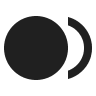
\includegraphics[scale=0.2]{img/record.png}
  \caption{Nahrávání cesty}\label{fig:record}
\endminipage\hfill
\minipage{0.32\textwidth}
  \centering
  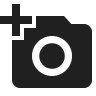
\includegraphics[scale=0.2]{img/camera.png}
  \caption{Přidání fotky}\label{fig:camera}
\endminipage\hfill
\minipage{0.32\textwidth}%
  \centering
  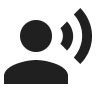
\includegraphics[scale=0.2]{img/recordsound.png}
  \caption{Nahrání zvuku}\label{fig:recordsound}
\endminipage
\end{figure}

Obrázky je od verze Androidu 5 možné specifikovat ve vektorovém formátu a odpadá tak dříve
nutné vytváření mnoha verzí stejného obrázku pro každou třídu rozlišení.
Z důvodu zpětné kompatibility pro verze nižší než 5 je přesto nutné tyto rastrové verze obrázků
vytvořit, nicméně vývojové nástroje již tento scénář předpokládají a tyto rastrové verze jsou
pro nižší verze systémy vygenerovány během kompilace, což značně zjednodušuje údržbu obrázků.



Pro další ikony loga aplikace a podobně byly použity zdroje ze služby
Iconfinder\footnote{\url{https://www.iconfinder.com/}  (10.4.2016)}, kde je licence pro použití také zdarma. V tomto
případě se jedná a Creative Commons Attribution 3.0 Unported (CC BY 3.0)
\footnote{Popis licence na \url{http://creativecommons.org/licenses/by/3.0/}  (10.4.2016)}, což je starší verze
licence popsané výše a v praxi jsou pak podmínky použití ikon stejné.




%  Rozměry

%  Kliknutí






\subsection{Použité nástroje}
Následující nástroje byly použity pro návrh, úpravy a správu projektu a značně pomohly při jeho vytváření.
\subsubsection{Trello (\url{https://trello.com}, 10.4.2016)}
Trello je jednoduchý online nástroj pro správu úkolů, jejich štítkování, zapisování poznámek a přesouvání
mezi různými seznamy reprezentujícími kategorii úkolů. V této práci bylo Trello použito pro lepší
rozvržení úkolů implementace a úseků psaní práce a přesto, že na projektu pracoval pouze jeden vývojář,
Trello mnoho věcí zpřehlednilo a psaní práce tak byla efektivnější. Logo nástroje můžeme vidět
na obrázku \ref{fig:trellologo}. Nástroj je přístupný zdarma a nabízí premium edici pro zpřístupnění
více funkcí. Pro naše potřeby verze zdarma zcela stačila.

\subsubsection{draw.io (\url{http://www.draw.io}, 10.4.2016)}
Online nástroj pro tvorbu grafů, všech různých typů diagramů, myšlenkových map a dalších.
Celý editor běží pouze v prohlížeči a synchronizuje vytvářené grafy s připojeným úložištěm
Google Drive nebo Dropbox. Grafy jsou tak přístupné  a editovatelné odkudkoliv a aplikace
je opravdu pokročilá a při práci není vůbec poznat, že vše probíhá pouze v prohlížeči.
Umožňuje sdílení i export zhotovených diagramů do mnoha formátů a je tedy velice snadné
sdílet a používat vytvořenou práci.
Nástroj byl použit pro vytváření veškerých diagramů a schémat v této práci.

\begin{figure}[H]
\begin{minipage}{.5\textwidth}
\centering
                
\includegraphics[scale=0.3]{img/trello-logo-blue.png}
        \caption{Logo nástroje Trello}
                \label{fig:trellologo}
                \centering Zdroj: \url{https://trello.com/home}
\end{minipage}
\begin{minipage}{.5\textwidth}
\centering
                
\includegraphics[scale=0.2]{img/drawiologo.png}
        \caption{Logo nástroje draw.io}
        \label{fig:iologo}
        \centering Zdroj: \url{http://www.draw.io}
    \end{minipage}
\end{figure}



\subsubsection{GIMP (\url{https://www.gimp.org/}, 10.4.2016)}
GIMP je široce používaný nástroj pro práci s obrázky a jejich úpravu. GIMP znamená
 \textit{GNU Image Manipulation Program}, což lze volně přeložit jako program pro práci s obrázky s GNU
 licencí, která nám říká, že program je zdarma a tudíž se hodí pro naše použití. GIMP nabízí obrovské
 množství funkcí a pro naše účely byl použit zejména pro úpravu snímků obrazovky užitých v této práci.


 \subsubsection{Android Asset Studio (\url{https://romannurik.github.io/AndroidAssetStudio/}, 10.4.2016)}
 Specifikem platformy Android je, že spoustu obrázků je potřeba držet v několika verzích pro optimální
 zobrazení na různých zařízeních, pro zdroje platí určitá pravidla a například poměr velikostí variant
 obrázků musí splňovat určitá kritéria. Udržovat a vytvářet tyto zdroje je často velmi obtížné
 a pomoci se nám s tím snaží nástroj Android Asset Studio, což je webová aplikace poskytující
 podporu pro vytváření obrázků v požadovaných velikostech, generování motivů aplikace a podobně.
 Pro naší aplikaci byl nástroj použit zejména pro generování ikon vyskytujících se v aplikaci
 a také pro generaci spouštěcí ikony, která podléhá jiným pravidlům než běžné ikony.


\subsection{Platforma Android}
Systém Android byl poprvé vypuštěn do světa v roce 2008 v útrobách zařízení T-Mobile~G1\cite{androidcentral}
a~díky své dostupnosti a otevřenému kódu rychle rozšířil a v současné době je to zcela jasně nejvíce využívaný mobilní
operační systém, který se stále bouřlivě vyvíjí. Jeho otevřenost je zároveň pro vývojáře i jedním z jeho problémů,
neboť výrobci si systém rádi upravují, v důsledku čehož se může aplikace na některých zařízeních chovat
neočekávaně a často se lze setkat se situací, že určitá funkce aplikace nefunguje správně právě na
jednom konkrétním typu zařízení.

Díky své rozšířenosti a dostupnosti se platforma Android nabízí jako dobrá možnost pro implementaci
aplikace na podporu cestování, neboť bude pro klienty snadno dostupná na zařízeních všech cenových
kategorií, kam si je mohou stáhnout přes obchod Google Play, kde může bude aplikace publikována.
Systém nabízí podporu pro velké množství různých senzorů, které dnešní mobilní zařízení obsahují
a tak je čtení dat z akcelerometru nebo zaznamenávání GPS řešeno pouze voláním příslušných metod
rozhraní frameworku. Během doby existence systému se objevilo také mnoho rozšiřujících knihoven
pro zjednodušení práce programátora umožnění vývoj aplikace efektivněji. Naše aplikace se
za pomoci těchto nástrojů pokusí zjednodušit mentálně postiženým klientům cestování po svých
obvyklých cestách.

Systém Android poskytuje vývojáři několik základních komponent, z nichž námi používané detailněji popíšeme.

\subsubsection{Záměr(\texttt{Intent})}
Platforma Android byla vymýšlena tak, aby vývojář místo explicitního spouštění konkrétní aplikace pro danou činnost
raději popsal záměr, co by chtěl udělat a systém sám vyhodnotí, která aplikace se pro tento záměr nejlépe
hodí. Touto cestou se systém snaží vytvořit prostředí mnoha aplikací, které spolu navzájem komunikují,
aniž by jedna o druhé přímo věděly a pomocí záměrů tak snižuje vazby mezi komponentami. Záměr může mít
textově popsanou obecnou akci, blíže specifikovanou kategorii, typ, mnoho dalších parametrů až po konkrétní
jméno komponenty, která má záměr obdržet, Pomocí těchto nastavení systém vyhodnotí nejlepší komponentu,
která má pro uživatele záměr vykonat. Při vyhodnocování záměrů systém využívá pro správný výběr
 tzv. filtry záměrů(\texttt{IntentFilter}).

Pokud chceme například odeslat email, nespouštíme emailovou aplikaci, ale vytvoříme záměr odeslat email
s příslušnými parametry a tento záměr předáme systému, který ze seznamu nainstalovaných aplikací vybere
ty, které dokážou náš email odeslat a v případě více výsledků nechá uživatele vybrat, která z aplikací
má záměr obdržet. Parametry záměru by v tomto případě byly předmět, adresát emailu a tak dále.

Naopak pokud chceme v aplikaci spustit některou z našich aktivit, dáváme aplikaci pomocí třídy
aktivity přesné jméno komponenty, kterou má spustit, nicméně samotnou aktivitu s jejím životním
cyklem vytvoří systém, nikoliv vývojář sám.

Pomocí záměru se předávají všemožné informace a může kromě zmíněných případů sloužit k vyvolání
vzdálené akce, informace o systémové události nebo pouze pro přenos dat, které musí být vždy
serializovatelné, neboť je tím umožněno systému záměr uchovat i v případě ukončení spouštěcího
procesu a předávání záměrů mezi procesy.

\subsubsection{AndroidManifest.xml}
Jedná se v o výpis všech veřejných informací aplikace ve formátu XML, které systém
a také uživatel potřebují o aplikaci vědět. Android manifest obsahuje identifikátor aplikace, deklaruje všechny
požadovaná povolení, podporované velikosti obrazovek zařízení nebo vyžadované funkce jako například přítomnost
fotoaparátu. Dále deklaruje podporované verze systému a v neposlední řadě také všechny hlavní komponenty
aplikace, jako například aktivity a služby a tím definuje všechny vstupní body aplikace a podmínky
jejich spuštění pomocí záměrů. Při publikování aplikace
parsuje Google Play tento soubor pro zobrazení informací pro záznam v obchodě a podobně instalační služba
systému Android, pro zobrazení ikony v seznamu aplikací a také vytvoření uživatele podle identifikátoru
aplikace a přiřazení přístupových práv pro konkrétní deklarovaná povolení.

\subsubsection{Aktivita}
Aktivita je komponenta aplikace, která obsahuje uživatelské rozhraní viditelné pro uživatele. Každá
 používaná aktivita aplikace musí být definována v Android manifestu se svými podmínkami pro své
 spuštění, neboli filtry záměrů(\texttt{IntentFilter}) a tím deklarovat vstupní místa do aplikace.
 Nejčastěji je v aplikaci jedna aktivita figurující jako spouštěč(akce záměru \texttt{MAIN},
 kategorie \texttt{LAUNCHER}), která se při
  instalaci vyhledá a vytvoří se pro ní spouštěcí ikona v seznamu nainstalovaných aplikací, další
  aktivity pak mohou mít explicitně definované vlastní filtry záměrů, případně nedefinovat žádný
  a tedy mít implicitně definovaný filtr na jméno třídy aktivity v kontextu balíčku aplikace.

 Třída aktivity, dědící ze systémové třídy \texttt{Activity},
 poskytuje vývojáři API se svým životním cyklem, skrz který by mělo být reagováno na to, v jakém
stavu se uživatelské rozhraní právě nachází. Pro akce při vytváření aktivity je používaná metoda
\texttt{onCreate}, která se volá pro každou instanci aktivity právě jednou a mělo by se v ní připravit
uživatelské rozhraní, získat příslušné služby a podobně. Aktivita je zobrazena uživateli po zavolání metody
\texttt{onResume} a v této chvíli může uživatel interagovat s uživatelským rozhraním. Pokud uživatel
přechází do jiné aktivity, přepíná aplikace, zamyká obrazovka nebo jiným způsobem opouští uživatelské
rozhraní, volá se metoda \texttt{onPause}. Pokud se zcela ukončuje používání konkrétní aktivity,
volá se metoda \texttt{onDestroy}, kde by se měly uvolnit všechny zdroje.
Celý životní cyklus aktivity můžeme vidět na obrázku \ref{fig:activitylyfecycle} a jedná se
často o první diagram, který vývojář pro platformu Android vidí.
Velmi častým problémem při vývoji je držení dat a podobných věci přímo v aktivitách,
neboť ta může být kdykoliv zničena systémem, například
pokud uživatel pouze otočí obrazovku a vyžaduje se v tu chvíli nové uživatelské rozhraní. Pokud v takové chvíli
někdo drží stále na aktivitu referenci, zničená instance aktivity není uvolněna z paměti a vzniká únik paměti.
Tento problém se stal ve světě vývojářů Androidu tak častý, že přímo pro jeho prevenci byla vytvořena knihovna
LeakCanary(\url{https://github.com/square/leakcanary}, 10.4.2016).
\begin{figure}[H]
        \centering
                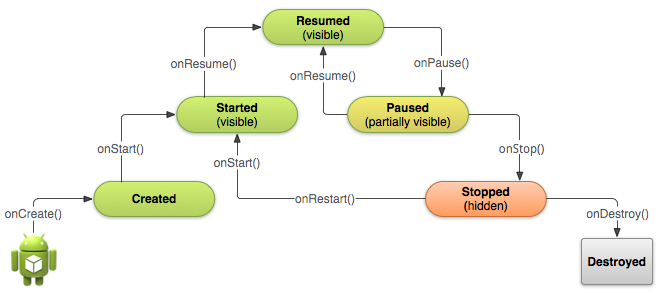
\includegraphics[scale=0.2]{img/basic-lifecycle.png}
        \caption{Životní cyklus aktivity}
        \label{fig:activitylyfecycle}
\end{figure}

\subsubsection{Fragmenty}
Fragmenty mohou být části uživatelského rozhraní aktivity nebo sloužit například pro předávání
dat mezi instancemi stejné aktivity například při rotaci. Fragmenty mají s aktivitou svázaný stejný životní cyklus
a všechny metody tohoto cyklu jsou provolávány do fragmentu. Jedna instance fragmentu
může být předávána mezi instancemi více aktivit a fragment tak může sloužit jako ideální komponenta
v případě, kde potřebujeme mít logiku svázanou s životním cyklem aktivity, chceme však jistá data
předat bezpečně mezi instancemi rotující aktivity, případně pokud chceme určitou část uživatelského
rozhraní udržet i při změně instance aktivity. Toto v aplikaci používáme například u map, kde pomocí
držení mapy ve fragmentu předcházíme novému načtení mapy při rotaci a tudíž nežádoucímu probliknutí.
Fragmenty byly představeny v Androidu verze 3 a zpočátku způsobily mnoho otázek a jejich správném využívání.
V současnosti se doporučuje využít je hlavně pro dynamické zobrazování uživatelského rozhraní na
zařízeních s různými obrazovkami\cite{androiddevelopers} a pro logiku patřící pouze uživatelskému rozhraní.

\subsubsection{Služby}
Služby jsou určeny pro operace, které nejsou viditelné uživateli, případně asynchronní operace, které se mají
provést bez vazby na rozhraní. Služby mají také svůj životní cyklus, nicméně odlišný a jednodušší,
než aktivity. Instance služeb, dědících ze systémové třídy \texttt{Service}, opět vytváří
systém a spravuje je po dobu jejich existence,
přičemž vývojář spouští služby záměry a pomocí nich jim předává také například data ke zpracování.
Služby se stejně jako aktivity musí registrovat v Android manifestu a mohou být součástí veřejného
rozhraní pro jiné aplikace. Pomocí deklarace v manifestu můžeme také definovat nový proces pro službu
a ještě více tak oddělit její spuštění od naší aplikace.

\subsubsection{Aplikace}
Při spuštění aplikace se vytvoří právě jeden aplikační objekt, kde může vývojář inicializovat
komponenty potřebné v celé aplikaci. Aplikace se opět deklaruje v manifestu jménem své třídy, která
dědí ze systémové třídy \texttt{Application}.



\section{Implementace}

\subsection{Nástroje použité pro vývoj}
Android je v současné době nejpoužívanější mobilní operační systém a programuje pro něj obrovské
množství vývojářů, kteří pro stále vyšší nároky na aplikace potřebují pracovat efektivně a Android samotný
a spoustu dalších společností pro ně poskytuje celou řadu nástrojů, které jim mají usnadnit práci a zefektivnit vývoj.

\subsubsection{Vývojové prostředí}
Přesto, že první verze Android vyšla již před 10 lety, získal Android své vlastní vývojové prostředí, Android Studio,
až v roce 2013 a na verzi 1.0 si vývojáři počkali až do konce roku 2014. Dříve byl vývoj řešen pluginy ve známých
vývojových prostředích jako Eclipse, NetBeans a později IntelliJ IDEA od JetBrains. Právě poslední jmenované
se časem stalo jedničkou a díky tomu, že existuje open source verze, posloužila IntelliJ jako základ pro Android Studio
a dodnes se změny pro IntelliJ dostávají postupně do Android Studia a naopak, takže se vzájemně stále obohacují.

S příchodem vlastního vývojového prostředí se vývoj značně zjednodušil a tým Android Studia neustále vylepšuje integraci s SDK,
nástroji pro sestavení, neboli build projektu a pluginy, kterých je celá řada a ten hlavní je Android Gradle Plugin
nad open source build systémem Gradle, umožňujícímu definici buildu v Groovy skriptech s možností využití Javy,
 pomocí něhož se celý projekt sestavuje a vytváří se aplikace se všemi dílčími kroky, které jsou pro to potřeba.
Pomocí Gradle pluginu se do procesu sestavení tyto kroky vloží, umožní se jejich konfigurace pomocí Gradle skriptů
a Android Studio slouží pouze jako obálka nad běžícím Gradle buildem, kdy vývojové prostředí řeší pouze nápovědy vývojáři,
napovídání, analýzu kódu a celkově vývojářovo pohodlí, neřeší však samotný build, který přenechává Gradlu a spuštění buildu
 z příkazové řádky je naprosto ekvivalentní buildu ve vývojovém prostředí, což znamená velkou výhodu při sestavování aplikace
 v cizích prostředích, například build serveru.
 Gradle také poskytuje velice užitečný mechanismus jménem Gradle Wrapper, což je spustitelný Java jar archiv,
 který je spolu s několika skripty uložen spolu s projektem a při spouštění buildu přes tyto skripty stáhne v rámci
 buildu nakonfigurovanou distribuci Gradlu na spouštějící stanici. Při distribuci kódu tedy stačí pouze spustit
 skript a vývojář se nemusí starat o jakoukoliv komplikovanou instalaci build systému.

 \subsubsection{Verzování kódu}
 Jako systém verzování byl použit Git, který je jeden z nejrozšířenějších verzovacích systémů a služba GitHub\url{https://github.com}(29.4.2016),
 která podporuje zdarma hostování open source repositářů s nabídkou mnoha služeb okolo, mimo jiné snadnou integraci se službou
 Travis CI, která byla použita pro průběžnou integraci projektu. Díky službě GitHub je zajištěno zálohování kódu
 během vývoje a díky Gitu je vyřešeno verzování se všemi výhodami, které to s sebou přináší, jako možnost vrátit se
 ke konkrétní verzi projektu, porovnávat a sledovat změny, případně vyvíjet několik funkcionalit nezávisle na sobě.
 Dále bylo pomocí těchto nástrojů řešeno uzavírání verzí publikováno na Google Play, kdy byl pro každou verzi vytvořen
 release, takže v případě, že se objeví problém u uživatele, jsme vždy schopní snadno dostat kód do stavu
 ve kterém je u uživatele a snáze tak najít a vyřešit problém. Stránku projektu na GitHubu lze nalézt na
 \url{https://github.com/jraska/Diploma-Thesis}(29.4.2016).

 \subsubsection{Průběžná integrace}
 Díky hostování projektu na GitHubu bylo možné snadné využití službu Travis CI(\url{https://travis-ci.org}, 10.4.2016),
 která se zaregistruje pro repositář
 a při každé změně spustí build celého projektu v uzavřeném prostředí, díky čemuž dokážeme okamžitě
 odhalit jakékoliv problémy, které se na naší stanici nemusí projevit, nicméně mimo naše prostředí ano.
 Služba stáhne veškerý kód z repositáře, nakonfiguruje uzavřený virtuální kontejner, nainstaluje Javu, Android SDK,
 případně další komponenty a spustí build projektu, v rámci něhož se spouští i unit testy. Služba se konfiguruje pomocí
 soubor \texttt{travis.yml} v kořenovém adresáři repositáře, v němž je specifikováno, že se projekt má sestavit jako Android projekt,
 jaký software se do prostředí má před každým během nainstalovat a co se má stát v případě chyby. Travis CI po stažení
 repositáře tento soubor vyhledá a na základě jeho obsahu provede požadované akce.
 Službu a historii buildů pro aplikaci Asistence cestování si můžeme prohlédnout na \url{https://travis-ci.org/jraska/Diploma-Thesis}  (10.4.2016).

 \subsubsection{Statická analýza kódu}

\noindent
 \textbf{Lint}


 Pro analýzu kódu a odhalování potencionálních chyb, problémů a nepoužívaných souborů je používán Lint,
  což je nástroj, který v projektu kontroluje dodržení sady poskytnutých pravidel a který
  je již součástí build procesu Androidu. Během buildu se vytváří Lint Report
  se všemi varováními a chybami, které byly v projektu nalezeny. Nástroj je konfigurovatelný pomocí
  Gradle skriptů projektu, případně souborem \texttt{lint.xml}, pomocí něhož lze některé chyby
  vynechat, případně změnit jejich prioritu například z chyby na varování.
  Lint dokáže odhalit spoustu chyb jako třeba zapomenutí potvrzení při editaci nastavení uživatele,
  nezavření databázového kurzoru, přítomnost nepoužitých obrázků v projektu a podobně.
  Jeho další velkou výhodou je rozšiřitelnost, kde si každý může napsat vlastní Lint pravidla pro to, na co chce být upozorněn
  a v případě knihoven začne Android Studio jejich pravidla automaticky používat a zvýrazňovat problémy uživateli
  přímo v editoru.
  Příkladem může být knihovna používaná pro logování Timber, která pomocí Lint pravidel
  kontroluje, zda je použita správně a dokáže tak předejít chybám za běhu.

\noindent
\textbf{Codacy}
\nopagebreak

Dalším použitým nástrojem je služba Codacy(\url{https://www.codacy.com/}, 10.4.2016), což je ve své podstatě
automatizována analýza kódu vyhledávající potenciální chyby a problémy, která se spustí po každé změně v kódu
díky opět snadné integraci s GitHubem. Služba odhaluje problémy jako nepoužívaný kód, příliš složité
třídy nebo metody, známé programátorské chyby či bezpečnostní rizika. Po analýze projekt oznámkuje podle
množství nalezených problémů v poměru k množství analyzovaného kódu. Aktuální analýzu projektu si můžeme prohlédnout
na \url{https://www.codacy.com/app/josef-raska/Diploma-Thesis/dashboard}(29.4.2016).

\subsection{Architektura}
Android samotný se snaží uživateli nabízet implementaci Architektury Model View Controller\cite{bestpracticesfuturice}, kde
každá akce rozhraní view směřuje na controller, který provede příslušnou logiku, případnou komunikaci
s modelem - vrstvou poskytující data,
kde se dá aktivita považovat jako controller\cite{mvcxmvp}, třídy dědící ze systémové třídy \texttt{View} která
se umí vykreslovat na obrazovku jako view a jako model nabízí systém mechanizmus poskytovatel obsahu
(\texttt{ContentProvider}), který umožňuje vytvořit v podstatě REST API nad SQLite databází.
Zejména pro část modelu se však tato část často implementuje zcela jinak, neboť uživatel nemá tímto způsobem
přímý přístup k databázi a poskytovatelé obsahu jsou tak často vhodní více pro komunikaci mezi aplikacemi,
kterou přístup k datům založený na URL poskytovatele obsahu umožňuje. Ohledně rozdělení na view a controller je opět
v platformě několik nejasností z důvodu nekonzistence API mezi verzemi, kdy ve verzi Androidu 3.0 přibyly
jako části aktivity fragmenty a u mnoha vestavěných tříd systému pro View vrstvu(například ListAdapter)
provádí i sám systém logiku patřící mimo View vrstvu a tento vzor není tedy striktně dodržováno a vzhledem
k nutnosti provazovat logiku načítání dat s životními cykly aktivit, které jsou zase svázané s uživatelským
rozhraním nelze tedy komponenty zcela precizně oddělit\cite{mvcxmvp}.
Schéma architektury MVC můžeme vidět na obrázku \ref{fig:mvc}.

\begin{figure}[H]
        \centering
                \includegraphics[scale=0.3]{img/mvc.png}
        \caption{Schéma architektury MVC}
        \label{fig:mvc}
\end{figure}

Díky specifikům platformy existuje mnoho odlišných přístupů, které se snaží přizpůsobit
tradiční architektury jako již zmíněný Model View Controller, případně podobný Model View, View Model
nebo Model View Presenter(MVP) a existuje mnoho projektů, která se snaží ukázat adaptaci těchto modelů
pro Android.

Pro náš projekt jsme vybrali architekturu Model View Presenter, která nám lépe umožňuje
úplné oddělení modelu od view a všechny aktualizace uživatelského rozhraní se provádí skrz presenter,
 což je v našem případě aktivita. MVP tak více připomíná vrstvenou architekturu, což nám vyhovuje, neboť
za vrstvou modelu mohou být další vrstvy komunikace s databází, případně po síti.

\begin{figure}[H]
        \centering
                \includegraphics[scale=0.3]{img/mvp.png}
        \caption{Schéma architektury MVP použité v projektu}
        \label{fig:mvp}
\end{figure}

Architektura projektu byla tedy volena s přikloněním k MVP, ve velké míře se používají
aktuální úspěšné knihovny a byl kladen důraz na následování známých principů SOLID, popsaných
například v \cite{solid} a IoC(Inversion of Control), popsaných v \cite{ioc} spolu s vkládáním
závislostí pomocí knihovny Dagger 2, kterou popisujeme v sekci \ref{dagger2}.
V projektu je na mnoha místech použito jednotkové testování pro podporu menší chybovosti v kódu
za pomocí nástroje Robolectric popsaného v sekci \ref{robolectric}. Přístup k datům a tedy
vrstva modelu s propagací výsledků do vyšších vrstev je realizována
 pomocí RxAndroid(sekce \ref{rxandroid}), kde se poskytuje přístup
presenterům k těmto datům pomocí objektů \texttt{Observable}. Presenter, tedy aktivita,
pak publikuje tato data do vrstvy view, kde objekty view zobrazí příslušná data. Fragment v našem
případě reprezentuje část view aktivity a je určen například k zobrazení nahrané cesty a všech informací,
které k ní byly přidány.

\subsection{Použité knihovny}
Jak již bylo zmíněno, Android používá velké množství vývojářů a pro jejich potřebu vzniklo velké množství
z drtivé většiny open source knihoven, tedy knihoven s volně přístupným kódem,
 které se snaží vyřešit a zjednodušit společný problém mnoha vývojářů
a usnadnit programování pro Android. Knihovny jsou díky tomu, že si může napsat knihovnu prakticky kdokoliv
různých kvalit a je proto nutné si každou napřed prohlédnout před jejím použitím, nicméně díky jejich
otevřenému kódu a hodnocením dalších uživatelů lze již nyní poměrně snadno najít spolehlivou knihovnu na téměř každý
typický problém, který při vývoji aplikací nastává a pročtením jejího kódu se ujistit, případně inspirovat,
jak dělat danou věc správně.

U některých knihoven je také zdůvodněno, proč jsou používány,
neboť mnohé řeší velice časté problémy vývoje, příčiny problematického kódu a je na nich založena
architektura aplikace.

\subsubsection{Android Support}\label{androidsupport}
Jedná se o základní knihovnu poskytovanou jako součást SDK, která řeší problémy kompatibility aplikace
mezi různými verzemi a sjednocuje jejich vzhled. Poskytuje také množství rozšiřujících komponent uživatelského rozhraní,
pomocné třídy například pro notifikace, média a spoustu dalších. V současné době by měla být součástí každé
aplikace a při vytváření nového projektu je k projektu již automaticky přidána.

Dokumentaci knihovny můžeme najít na \url{http://developer.android.com/tools/support-library/index.html}  (10.4.2016).

\subsubsection{Dagger 2 a vkládání závislostí}\label{dagger2}
Poměrně nová knihovna spravovaná Googlem a uvolněná poprvé v srpnu 2015, která pro nás řeší tzv. vkládání
závislostí(anglicky Dependecy Injection) do objektů,
které tyto závislosti chtějí používat. Knihovna je použita za účelem zkvalitnění kódu a zlepšení testovatelnosti, jelikož
je v celém projektu následována filozofie, že třídy by měly objekty buď vytvářet a nebo používat. To v podstatě znamená,
že se snažíme omezit situace, kdy si třída v rámci své metody vytváří vlastní objekty, které potřebuje k vykonání
dané operace a zejména se se snaží úplně eliminovat situace, kdy si třída své závislosti sama začne vybírat z nějakého
kontejneru, statických proměnných a podobně. Jako špatný přístup je v tomto případě brán i často používán návrhový vzor
Jedináček, jelikož se jedná v podstatě o sdílený globální stav. Všechny objekty by měly své závislosti obdržet v konstruktoru
a neměly by se vyskytovat žádné metody tipu inicializuj objekt, nastav proměnnou, bez které objekt nemůže fungovat a podobně.

Cílem tohoto přístupu je zaručit jakémukoliv klientovi třídy, tedy programátorovi používajícímu její rozhraní,
záruku, že pokud získá referenci na tento objekt, bude vždy ve stavu připraveném pro použití a nemůže se mu stát,
že při volání některé z metod obdrží chybu, že zapomněl něco nastavit. Myšlenkou je, že programátor používající
tuto třídu musí pro její použití vidět pouze konstruktor a následně její rozhraní a nemusí pátrat, zda musí po
vytvoření objektu něco nastavovat. Kromě toho tento přístup výrazně zjednodušuje testovatelnost třídy, jelikož v rámci
Android testů běží všechny testy v jednom virtuálním stroji, mají tedy sdílenou paměť, což znamená, že statický
stav zůstává sdílen mezi testy, rozbíjí filozofii izolovanosti testů a může vyústit v situaci, kde jeden test selže,
jelikož nějaký jiný test před ním nastavil něco do globálního stavu.

Často je však tuto filozofii poměrně složité následovat, jelikož aby mohl programátor vytvořit objekt, který
v dané situaci potřebuje, musí mít přístup ke všem jeho závislostem, což může být obtížné zajistit
a vyvstává diskuze, kde odkazy na tyto objekty držet, jak je zpřístupnit všem potenciálním klientům třídy
a jak toto udělat přehledně bez toho, aniž by bylo vše vytvářeno na jednom místě. Toto může vyústit v techniky
jako je lokátor služeb, již zmíněný Jedináček a podobné, kdy si třída sama ve své implementaci potřebnou
závislost vytáhne, čemuž bychom chtěli předejít.
Android nám tento problém také značně stěžuje tím, že hlavní komponenty aplikace jako aktivity, služby a objekt
aplikace samotné jsou provázány co nejvolněji a nelze jednoduše předat jeden objekt z aktivity do aktivity,
dokud se nejedná o primitivní typ, případně jej lze serializovat.

Tento problém pro nás řeší knihovny pro vkládání závislostí, které se nám snaží umožnit to, že si o potřebné
závislosti prostě požádáme a knihovna nám je poskytne. My však musíme knihovně říct, jak tyto závislosti může
získat a kde je má uložit. Dagger 2 používá objekt nazvaný \texttt{Component}, což je kontejner závislostí
který dokáže vytvářet námi požadované objekty i s jejich závislostmi. Kontejner se skládá z modulů, které
za podmínky určitých vstupů poskytnou kontejneru nové výstupy. V kódu se tyto třídy definují pomocí anotací
a kód pro vytvoření kontejneru závislostí, nebo také objektového grafu, je vygenerován během kompilace
a díky tomu se za běhu vytvoří velmi rychle, což je jeden z hlavních důvodů, proč je Dagger 2 používá,
protože za běhu vůbec nepoužívá reflexi, která je u knihoven tohoto typu častá a která způsobuje v Android
aplikacích značné výkonnostní problémy. Knihovny pro vkládání závislostí existovaly již mnohem dříve,
jako například Spring nebo Guice, při použití na platformě Android byly však díky reflexe pomalé a mohlo snadno
dojít k chybě za běhu. Oproti tomu Dagger 2 vytváří objektový graf během kompilace, zkontroluje zda je acyklický,
všechny požadované závislosti je možné získat a v případě aplikace nám neumožní aplikaci úspěšně zkompilovat,
díky čemuž minimalizuje možné pády aplikace v případě nesprávného použití knihovny.

Dokumentaci a popis knihovny můžeme nalézt na \url{http://google.github.io/dagger/}  (10.4.2016).

\subsubsection{RxAndroid}\label{rxandroid}
Jedná se o Android rozšíření známé knihovny RxJava, která implementuje reaktivní rozšíření
mnohých programovacích jazyků sdružené pod projekt ReactiveX(\url{http://reactivex.io/}, 10.4.2016).
Knihovna k Java implementaci pouze přidává vlastnosti specifické pro platformu Android a to konkrétně
řešení spouštění metod v hlavním vlákně uživatelského rozhraní. Knihovna je založena na návrhovém
vzoru Pozorovatel(Observer) a její záměr je implementovat reakce na události bez vědomí, kdy přesně
událost nastane, ale s vědomím, že v tuto chvíli bude registrovaný pozorovatel na tuto událost
upozorněn a zareaguje na ni. Knihovna nabízí spoustu metod, jak na události reagovat, shlukovat je do
skupin, mapovat objekty výsledku na jiné, řeší příliš mnoho požadavků v jednom čase a spoustu dalších vlastností.
Jedná se o poměrně mocný nástroj, který nicméně vyžaduje nemálo času na nastudování, pochopení a v případě
Android platformy platí, že s velkou sílou přichází velká zodpovědnost, jelikož při registrace pozorovatele
se často v rámci registrace drží reference na aktivitu, což může v případě například rotace způsobit únik paměti,
případně i pád aplikace v důsledku pokusu o aktualizaci uživatelského rozhraní, které v té době už nemusí být dostupné.

RxAndroid navíc řeší další, pro Android velmi významný problém a tím je výběr vlákna, ve kterém se
operace spouští. Jako hlavní vlákno totiž slouží vlákno uživatelského rozhraní, které by
nemělo provádět žádné, byť jen trochu náročné operace, neboť by se vše mělo stihnout během 16ms\cite{perf}.
V aplikacích i knihovnách toto vede k obrovskému množství asynchronních zpětných volání, které mají různá jména,
každá knihovna si je řeší po svém, není nad nimi kontrola a výsledkem je nepřehledný asynchronní kód,
ve kterém se lze jen složitě orientovat. Díky RxAndroid a jejich implementaci plánovačů, lze rozhodnutí,
na jakých vláknech bude operace spuštěna a na kterém vlákně bude doručen výsledek nechat na klientovi třídy
a tím pádem například řetězit synchronní volání, pokud jsme již v asynchronním vlákně a zejména zajistit,
že výsledek obdržíme ve vlákně uživatelského rozhraní. Typická ukázka využití této vlastnosti
lze vidět na ukázce kódu \ref{rxmainthreaddeliver}, kde se získá seznam cest, operace pro jeho získání,
které jsou časově náročné se spustí v jiném vlákně a výsledek bude doručen na hlavní vlákno,
kde spustí poskytnutou metodu.


\begin{lstlisting}[label=rxmainthreaddeliver,caption=Reakce na událost v UI vlákně pomocí RxAndorid]
    ...
    routesRepository.selectAll()
        .subscribeOn(Schedulers.io())
        .observeOn(AndroidSchedulers.mainThread())
        .subscribe(this::setRoutes);
  }

  void setRoutes(List<RouteData> routes) {...}
\end{lstlisting}

Výhody reaktivního programování můžeme ocenit i při testování, které je typicky s asynchronním
rozhraním testované třídy problematické, nicméně díky RxAndroid volání \texttt{toBlocking()} vynutíme
synchronní spuštění požadované operace, což nám výrazně zjednoduší testování.

Knihovnu můžeme nalézt na \url{https://github.com/ReactiveX/RxAndroid}  (10.4.2016).

\subsubsection{Retrolambda}
Lambda výrazy jsou mocným nástrojem a příjemnou pomůckou každého jazyka, který je podporuje a redukují
často dlouhé bloky kódu do kratších, přehlednější funkcí. Jelikož Android kvůli zpětné
kompatibilitě podporuje pouze Javu 7
\footnote{Vyjma \texttt{try-with-resources}, které je podporováno až od verze Androidu 5.0.}
a lambda výrazy byly do Javy přidány až ve verzi 8, nemůže tyto funkce vývojář využívat,
což vede často k velkému množství anonymních tříd pro zpětné volání mnoha metod, jako typicky klepnutí,
vrácení načtených asynchronních dat nebo při registraci posluchače u výše zmíněné knihovny RxAndroid.
Tyto anonymní třídy značně ztěžují čitelnost kódu a velmi často vedou také k únikům paměti,
neboť anonymní třída drží implicitně referenci na instanci třídy, ve které je vytvářena, což je často
aktivita nebo jiný objekt, který by měl být z paměti jinak odstraněn.

Retrolambda umožňuje lambda funkce využít i v rámci kódu podporujícího pouze Javu 7,
čímž Android vývojáři umožňuje zbavit se anonymních tříd a využít potenciálu lambda funkcí
ve své aplikaci při zachování zpětné kompatibility s bytekódem Javy 7. Pro její využití je třeba
nastavit kompilaci projektu na verzi Javy 8 a do Gradle skriptů přidat plugin knihovny. Použité
lambda výrazy se během Java 8 kompilace přeloží do bytekódu, vyžadující její běhové prostředí,
nicméně tento nástroj transformuje bytekód do instrukcí, které jsou dostupné v běhovém prostředí
Javy 7 a pokud je to možné, provede další optimalizace pro ušetření vytváření instance objektu
pro každé volání.

Ukázku odstranění anonymní třídy můžeme vidět na ukázce kódu \ref{useretrolambda}.

\begin{lstlisting}[label=useretrolambda,caption=Odstrnění kódu anonymní třídy pomocí knihovny Retrolambda]
   saveButton.setOnClickListener(new View.OnClickListener() {
         @Override
         public void onClick(View v) {
           save();
         }
       });

            ▼                ▼

  saveButton.setOnClickListener(v -> save());
\end{lstlisting}

Knihovnu můžeme nalézt na \url{https://github.com/orfjackal/retrolambda}  (10.4.2016).

\subsubsection{Lombok}
Lombok je další z nástrojů který rozšiřuje jazyk Java, respektive se nás snaží ušetřit obvyklých
ceremonií jako implementace metod \texttt{equals, hashCode, toString}, implementaci přístupových
metod k datům třídy a podobně. Moderní vývojová prostředí včetně Android Studia toto vše umí
vygenerovat, nicméně při každé úpravě třídy se musí myslet na to, že je třeba příslušné metody
vygenerovat znovu, aby zůstaly aktuální, což může vést k chybám.

Lombok pomocí anotací u příslušné třídy vygeneruje během kompilace obvyklých metod a díky Lombok
pluginu do Android Studia nám vývojové prostředí tyto generované metody automaticky nabízí a díky tomu,
že se metody generují během každé kompilace, generované metody zůstanou vždy aktuální. Jednoduchá datová
třída se dvěma vlastnostmi z ukázky kódu \ref{lombokshowcase} se všemi korektně napsanými implementacemi
metod objektu \texttt{equals, hashCode, toString} a přístupových metod má délku kolem 50 řádků, nicméně
díky tomuto nástroji lze totožnou funkcionalitu napsat jen na 5 řádků, jak vidíme na ukázce \ref{lombokshowcase},
navíc s benefitem, že pro přidání další vlastnosti do všech metod stačí přidat pouze řádek vlastnosti
a promítne se korektně do všech dříve zmíněných metod.

\begin{lstlisting}[label=lombokshowcase,caption=Datová třída používající Lombok]
   @lombok.Data
   public class Position {
     private double latitude;
     private double longitude;
   }
\end{lstlisting}

Nástroj navíc poskytuje další užitečné anotace, například \texttt{@Value} pro generování neměnitelných objektů
bez přístupových metod, \texttt{@Builder} pro generování stavitelů objektů pro eliminaci konstruktorů s velkým
počtem parametrů, případně \texttt{@SneakyThrows}, který nás zbavuje nutnosti obalovat kontrolované výjimky
\texttt{try-catch} blokem případně výjimku propagovat do signatury metody a mnohé další.

Stránky Lomboku můžeme nalézt na \url{https://projectlombok.org/}  (10.4.2016).

\subsubsection{Google Play Services}
Soubor knihoven od Googlu, které se snaží vývojáři rozšířit možnosti implementace všemi různými způsoby.
Obsahuje například knihovny pro rozpoznávání obličeje a nálady, plánování úloh, podporu monetizace aplikace,
mnohé další a také námi používané rozhraní na upozornění přiblížení se k určitému místu a také Google Drive API.

Jedná se v podstatě o rozšiřující API celého frameworku, které by mělo být dostupné na každém zařízení, které
obsahuje aplikaci obchodu Google Play a tudíž na všech zařízeních, kde je možné naší aplikaci stáhnout.
Knihovna je zároveň přes aplikaci obchodu aktualizovaná a tudíž u ní nemusíme řešit problémy
kompatibility, jako u vlastního SDK. \cite{gms}

Přehled všech rozhraní lze nalézt na \url{https://developers.google.com/android/guides/overview}  (10.4.2016).

\subsubsection{Butter Knife}
Jedná se o knihovnu, která nás zbavuje dalších ceremonií Androidu nastavování posluchačů
na události objektů uživatelského rozhraní, jako klepnutí, změnu textu a podobně. Knihovna pomocí
anotací nad požadovanými metodami tyto posluchače a jejich nastavování generuje a my těmito anotacemi
pouze specifikujeme, co se má během dané události stát. Ukázku zobrazování nápovědu u obrázků, která je
používána v aplikaci, můžeme vidět na ukázce \ref{butterknife}.

\begin{lstlisting}[label=butterknife,caption=Použití knihovny Butter Knife]
  @OnLongClick(R.id.navigate) boolean showContentDescription(View v){
    return ViewUtils.showContentDescription(v);
  }

\end{lstlisting}

Knihovnu můžeme najít na \url{http://jakewharton.github.io/butterknife/}  (10.4.2016).

\subsubsection{DBFlow}\label{dbflow}
Jedné se o knihovnu pro objektově relační mapování objektů pro databáze SQLite, které se v
 Androidu používají jako výchozí. Práce s touto databází pomocí API Androidu není
 složitá, nicméně kód je poměrně zdlouhavý a pro přečtení nebo uložení objektu je potřeba
 mnoho řádek kódu. Pro objektově relační mapování existuje mnoho knihoven, najít mezi nimi takovou,
 která by vyhověla všem požadavkům, je velice obtížné. Velká většina těchto knihoven využívá reflexi,
 která svou časovou náročností může překonat i operace zápisu a čtení z databáze.
 DBFlow se snaží tento problém řešit generací kódu pro čtení a zápis dat pomocí anotací nad objekty
 a jejich vlastnostmi, následně jejich ukládání řeší pomocí adaptérů vygenerovaných pro každou anotovanou
 třídu a SQL dotazy se píší pomocí generovaných metod a metod knihovny. DBFlow není také ideální
  a nutí vývojáře používat jejich bázovou třídu pro mapované objekty, případně implementovat vlastní
  adaptér a některé databázové vazby se pomocí anotací nedefinují nejlépe, nicméně pro nás projekt
  knihovna zcela vyhovuje a vygenerovaný kód práce s databází se velice podobá tomu, který by vývojář
  sám musel psát. Ukázka sestavování SQL dotazů pomocí DBFlow můžeme vidět na ukázce \ref{dbflowquery}.

\begin{lstlisting}[label=dbflowquery,caption=Sestavování SQL dotazů s DBFlow]
  RouteData select(long id){
    return SQLite.select().from(RouteData.class)
            .where(RouteData_Table._id.eq(id)).querySingle();
  }
\end{lstlisting}

  DBFlow nám také umožňuje přidávat adaptéry pro vlastní datové typu a tím nám umožnit uložit
  typ do jednoho sloupce, kde by si bez adaptéru knihovna neuměla poradit. V aplikaci
  tohoto využíváme pro uložení identifikátorů \texttt{UUID} a také objektů \texttt{LatLng},
  které obsahují GPS souřadnice a adaptér je ukládá jako text oddělený čárkou.
  Knihovna obsahuje také některé vestavěné adaptéry pro často potřebné objekty, například námi
  také využívaný objekt \texttt{Date}.

  Další podporovanou funkcí jsou migrace, kde se opět pouze anotacemi dá definovat třída,
  která má migraci databáze na novou verzi převést.

  Knihovnu můžeme najít na \url{https://github.com/Raizlabs/DBFlow}  (10.4.2016).


\subsubsection{Robolectric}\label{robolectric}
Jednotkové testy využívající kód Androidu je poměrně zdlouhavé spouštět, neboť kód běží na
zařízení a pro každé spuštění testu se musí sestavit nové testovací APK, nahrát na zařízení
a až poté spustit testy. Pokud se programátor pokusí spustit testy na svém počítači s využitím
SDK Androidu, obdrží při prvním použití výjimku, neboť SDK obsahuje pouze deklarace metod
bez implementací a skutečné implementace jsou pouze na zařízení.

Robolectric se snaží toto řešit pomocí emulace SDK Androidu na počítači a umožnit tak vývojáři
testovat svůj kód bez nahrávání na zařízení a výrazně tak zrychlit testování. Robolectric
používá tzv. stínové objekty pro všechny třídy SDK a pomocí nich lze emulovat systémové události,
získávat systémové objekty a případně nahrazovat některé vlastní implementací pro simulaci
určitých podmínek. Knihovna se vyvíjí už mnoho let a díky záměru simulovat celý framework je velmi
rozsáhlá a zatím stále ne zcela dokonalá, nicméně se stala standardem pro testování Android kódu
přímo na pracovní stanici.

Knihovnu lze nalézt na \url{http://robolectric.org/}  (10.4.2016).

\subsubsection{Další použité knihovny}
\begin{itemize}
  \item \textbf{Universal Image Loader} - Práce s obrázky a fotkami. (\url{https://github.com/nostra13/Android-Universal-Image-Loader}  (10.4.2016))
  \item \textbf{Timber} - Logování zpráv v aplikaci. (\url{https://github.com/JakeWharton/timber}  (10.4.2016))
  \item \textbf{Okio} - Efektivní a snadné práce se soubory a datovými proudy. (\url{https://github.com/square/okio}  (10.4.2016))
  \item \textbf{EventBus} - Snadné publikování a konzumování globálních události v aplikaci. (\url{http://greenrobot.org/eventbus/}  (10.4.2016))
  \item \textbf{ShowcaseView} - Zobrazení uživatelsky přívětivé nápovědy. (\url{https://github.com/amlcurran/ShowcaseView}  (10.4.2016))
  \item \textbf{JUnit 4} - Známý framewrok pro Java jednotkové testy. (\url{http://junit.org/}  (10.4.2016))
  \item \textbf{AssertJ Android} - Pomocné aserce pro jednotkové testy. (\url{http://square.github.io/assertj-android/}  (10.4.2016))
  \item \textbf{Mockito} - Mockovací knihovna pro jednotkové testy. (\url{http://mockito.org/}  (10.4.2016))


\end{itemize}

\subsection{Volání o pomoc}
Během cestování se klient může dostat do různých situací a naše aplikace by mu měla umožnit rychle se
spojit se svým asistentem pro vyřešení problému, případně mu poslat zprávu. Asistent může v aplikaci nastavit své kontaktní
údaje a aplikace může následně tyto údaje využít k rychlému kontaktování. Klepnutím ikony kontaktovat
asistenta se klientovi zobrazí tlačítka s možnostmi.

\subsubsection{Volání asistentovi}
Pokud má uživatel v aplikaci uloženo číslo asistenta, po klepnutí na možnost volat se automaticky
vytočí jeho číslo a spustí se vytáčení. Hovor je v tuto chvíli zpoplatněn jako jakýkoliv jiný hovor
z telefonu uživatele.

\subsubsection{Odeslání SMS}
Pokud klient zvolí tuto možnost, vytvoří se SMS zpráva s textem, obsahující odkaz na Google mapy
se zakódovaným ukazatelem na místo, kde se klient nacházel v odesílání zprávy. Asistent si tak po obdržení
SMS zprávy může snadno zobrazit, kde se uživatel, který má problémy nachází. při vytváření a posílání zprávy
dbá aplikace na t, aby zpráva neobsahovala více než 160 znaků a klient tak zaplatil pouze za jednu SMS.

\subsubsection{Poslání emailu}
Podobně jako při odesílání SMS je připravena zpráva s odkazem na Google mapy, která opět asistentovi
umožní rychlý přístup k aktuální pozici uživatele. Vytvoří se záměr pro odeslání emailu s předvyplněnou
adresou asistenta, pokud je tato adresa v nastavení a spustí se emailová aplikace na zařízení pro odeslání
emailu z klientova emailového účtu. Spouštění emailové aplikace na zařízení nám umožňuje nepožadovat
od uživatele jeho zabezpečovací údaje k emailové schránce, což by bylo pro uživatele velmi nepříjemné.



\subsection{Nahrávání cesty}
Během nahrávání cesty se sbírají GPS souřadnice bodů, kterými uživatel se zařízením prochází,
k nim se přidávají další data jako fotografie, zvukové nahrávky poznámky,
případně informace o změně dopravního prostředku. Tyto data mají vždy přiřazenou zaznamenanou
GPS pozici, která později určí, kdy bude klient na tato data upozorněn.

Při spuštění nahrávání se spustí služba pro nahrávání pozice, která zaregistruje
posluchače na systémovou službu poskytující GPS souřadnice a při obdržení těchto souřadnic
vyšle po aplikační sběrnici událostí událost o nové pozici. Na této sběrnici jsou v tuto chvíli
registrování všichni, kteří tuto informaci potřebují znát, což je v tuto chvíli uživatelské rozhraní
zobrazující mapu a služba ukládající GPS souřadnice do seznamu, který je v případě, že se uživatel
rozhodne cestu uložit uložen do databáze. Jako systémová sběrnice se používá knihovna EventBus a pro
možnost registrovat posluchače na poskytovatele GPS souřadnic potřebuje naše aplikace povolení
získávat lokaci zařízení.

\subsubsection{Pořizování fotek}
Během nahrávání cesty může uživatel pořizovat svým telefonem fotky, které by klientovi při asistenci
cestování měly pomoci v orientaci a připomenout mu důležité body cesty. Při kliknutí na ikonku přidat
fotografii se vytvoří záměr pořídit fotografii s místem požadovaného uložení, spustí se
výchozí aplikace fotoaparátu na zařízení a o pořízení aplikace se nestará naše
aplikace, nýbrž aplikace, na kterou je uživatel zvyklý. Pokud uživatel pořídí fotku a rozhodne se jí
uložit, naše aplikace o tom obdrží zprávu, zobrazí se dialog, kde může uživatel fotografii pojmenovat,
vytvoří se unikátní identifikátor fotografie a příslušný záznam asociovaný s nahrávanou cestou,
přiřadí se mu aktuální pozice a v případě uložení cesty se tento záznam uloží spolu s cestou.

Jelikož fotografie mohou zabírat poměrně velké množství paměti, vysílá se v případě mazání cesty po
systémové sběrnici událost o mazání cesty na kterou čeká objekt promazávající všechny fotografie
a zvukové nahrávky, asociované s touto cestou.

\subsubsection{Pořizování zvukových nahrávek}
Při nahrávání může uživatel pomocí mikrofonu svého zařízení pořídit zvukovou nahrávku, které se bude
vztahovat k aktuálnímu místu, kde byla nahrávka pořízena a může klientovi poskytnout zvukovou
informaci hlasem, který je mu známý a sdělit mu obsáhlejší informace, které by bylo zdlouhavé číst.
Pokud uživatel klepne na tlačítko nahrávaní zvuku, spustí se obrazovka ukazující probíhající nahrávání
a začne se zaznamenávat zvuk, dokud uživatel neklepne na tlačítko zastavit nebo nezmáčkne tlačítko zpět.
V okamžiku otevření aplikace se vytvoří soubor, do kterého systémová služba pro nahrávání
zvuku začne zapisovat zvuk ve formátu 3GP.
Pokud uživatel ukončí nahrávání, může nahrávku pojmenovat a uložit. Té se následně přiřadí unikátní
identifikátor asociovaný s uloženým souborem a nahrávané cestě se přiřadí záznam přiřazující tuto
nahrávku dané cestě. V případě, že uživatel zvolí neukládat nahrávku, nahraný soubor se smaže.
Podobně jako v případě fotek jsou při smazání cesty vyčištěny i nahrávky pro zamezení plýtvání místem
na úložišti.

\subsubsection{Přidávání poznámek}
Kdykoliv během nahrávání může uživatel přidat textovou poznámku spojenou s aktuální polohou.
 Poznámka se zadává do dialogového okna a je poté uložena se zaznamenanou GPS pozicí, ve které byla napsána.

\subsubsection{Změna dopravního prostředku}
Zvláště se dá uložit změna způsobu transportu uživatele a to klepnutím na tlačítko zobrazující
aktuální dopravní prostředek. Pokud například uživatel jde na zastávku, má zobrazenou ikonu chodce,
pokud nastoupí do tramvaje a klepne na ikonu chodce, zobrazí se mu nabídka pro změnu dopravního
prostředku a klepnutím na ikonu tramvaje se tato změna uloží opět s vazbou an aktuální GPS polohu.
Uživatel může k této informaci přidat také textový popis například s číslem tramvaje nebo jiné instrukce.
Tyto informace se uloží jako záznam do databáze s vazbou na nahrávanou cestu v místě, kde byl záznam pořízen.
Ikony používané pro vyjádření druhů dopravních prostředků můžeme vidět na obrázcích \ref{fig:icwalk},
\ref{fig:icbus} a \ref{fig:ictram}.

\begin{figure}[H]
\minipage{0.32\textwidth}
  \centering
  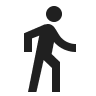
\includegraphics[scale=0.2]{img/ic_directions_walk_black_24dp.png}
  \caption{Ikona chůze}\label{fig:icwalk}
\endminipage\hfill
\minipage{0.32\textwidth}
  \centering
  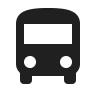
\includegraphics[scale=0.2]{img/ic_directions_bus_black_24dp.png}
  \caption{Ikona autobusu}\label{fig:icbus}
\endminipage\hfill
\minipage{0.32\textwidth}%
  \centering
  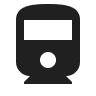
\includegraphics[scale=0.2]{img/ic_directions_railway_black_24dp.png}
  \caption{Ikona tramvaje}\label{fig:ictram}
\endminipage
\end{figure}

Změna dopravního prostředku je také místo pro budoucí vylepšení, neboť je možné pomocí akcelerometru
zařízení a rozpoznávání statistických vlastností hodnot zaznamenaných akcelerometrem určit tuto informaci
automaticky bez účasti uživatele. Knihovna Google Play Services také podporuje API, které se pokouší
poskytnout uživateli tuto informaci.


\subsection{Zobrazení nahrané cesty}
Nahranou cestu je možné uživateli na zařízení zobrazit a umožnit tak kontrolu a prohlížení dat.
Pro zobrazení slouží fragment mapy ve kterém se zobrazí spojená čára propojující jednotlivé body.
Vzhledem k nepřesnostem a šumu při nahrávání však jako cesta často vzniká velmi lomená čára a dojem z vykreslení
na mapě není dobrý. Z tohoto důvodu byla implementováno vyhlazování čar pomocí prokládání aproximační
B-spline křivkou, algoritmem inspirovaným v \cite{bspline}. B-spline křivka je počítána podle
rovnice \ref{eq:bspline}, kde je výsledná křivka vytvořena vždy podle 4 sousedních bodů $P_0$, $P_1$,
$P_2$ a $P_3$.

\begin{equation}
B(t)=\frac{(-P_0 + 3P_1 - 3P_2 + P_3)t^3}{6} + \frac{(P_0 - 2P_1 + P_2)t^2}{2} + \frac{(-P_0 + P_2)t}{2} + \frac{(P_0 + 4P_1 + P_2)}{6}
\label{eq:bspline}
\end{equation}
\centerline{Zdroj v \cite{bspline}}
\vspace{0.2cm}


Rovnice \ref{eq:bspline} se aplikuje zvlášť na GPS souřadnice zeměpisné šířky a délky s krokem $dt = 0.2$,
 což znamená, že ke každému bodu nám vznikne místo jednoho pět aproximací s okolními body a výsledná
 vykreslená čára je poté hladší, jak můžeme vidět na obrázku \ref{fig:splinediff}, kde je žlutou barvou
 vykreslena čára hrubých dat, uložených u nahrané cesty a modrou barvou je vykreslena čára s aplikovanou
 B-spline aproximací. Jak můžeme vidět, aproximace vyhladila ostré okraje zejména u změn směru.

\begin{figure}[H]
        \centering
                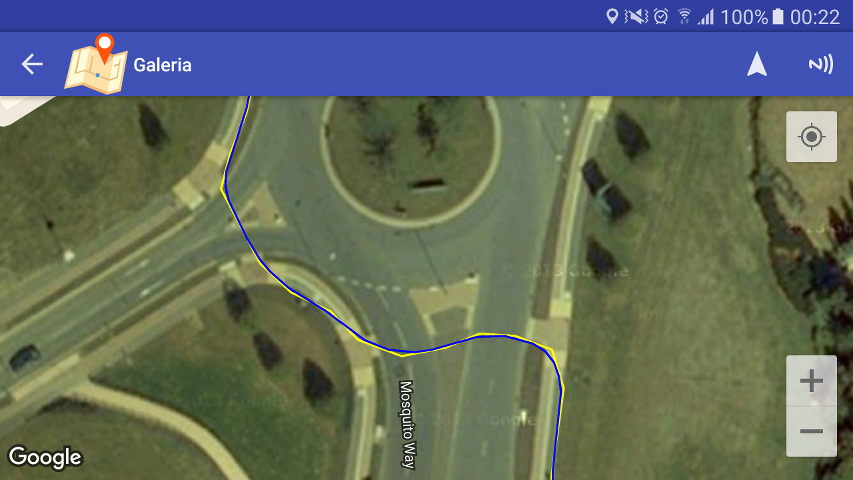
\includegraphics[scale=0.3]{img/screen/bsplineapplied.png}
        \caption{Vyhlazení křivky cesty pomocí B-spline aproximace}
        \label{fig:splinediff}
\end{figure}

Na mapě jsou dále zobrazeny všechny další data nahraná při cestě. Fotky se nahrají jako miniatury do paměti,
oříznou se a zobrazí se jako kruhový výřez nad místem, kde byla fotka pořízena.
Velikost miniatury je zadána jako 48dp pro zachování přibližně stejné velikosti na všech zařízeních.
Obrázky jsou nahrávány asynchronně pomocí knihovny Universal Image Loader a kruhové oříznutí se realizuje
pomocí implementovaného pre-processoru knihovny, která nahranou bitmapu ořízne do kruhového tvaru.
Při kliknutí na miniaturu fotky se opět asynchronně načte obrázek do dialogového okna,
které zaplní celý displej zařízení s poloprůhledným pruhem, ve kterém je napsán uložený titulek fotky.

Pro zvukové nahrávky a poznámky se zobrazí jednoduchá značka na mapě v místě, kde byla pořízena a při
klepnutí na značku se pouze v malém dialogovém okně zobrazí popis a v případě přítomnosti nahrávky
se načte z úložiště soubor nahrávky a spustí se. Pro změny cestování se v době zobrazování cesty do mapy
zobrazí z výčtu miniatury ikon, příslušných k zaznamenaným datům z změně dopravního prostředku.

\subsection{Asistence uživatele na cestě}
Pokud uživatel spustí asistenci na cestě, spustí se aktivita navigace, která načte z uložených
dat všechny informace, spustí GPS pro obdržení aktuální polohy a připraví vše, co je pro asistenci potřebné.
Navádění uživatele je pravděpodobně nejkomplexnější proces aplikace, jehož hlavním řídícím prvkem
je třída \texttt{NavigationActivity}, která
pomocí svých závislostí řeší několik základních úloh, jako je načtení a zobrazování cesty s aktuální polohou uživateli,
nabízení následujícího směru, přípravu událostí při přiblížení k místu, kde byl pořízen záznam a upozornění
uživatele v případě přiblížení k těmto místům. Zjednodušený třídní diagram se závislostmi třídy \texttt{NavigationActivity}
můžeme vidět na obrázku \ref{fig:navigationactivitydependencies}, který bude následně blíže popsán.

\begin{figure}[H]
        \centering
                \includegraphics[scale=0.2]{img/NavigationActivity.png}
        \caption{Diagram závislostí řídící třídy asistence \texttt{NavigationActivity}}
        \label{fig:navigationactivitydependencies}
\end{figure}

Řídící třída \texttt{NavigationActivity} dostává při svém spuštění jako parametr id cesty,
pro níž má asistenci spustit. Pomocí \texttt{TravelDataRepository} načte asynchronně data k této třídě
do paměti a provede všechny úkony potřebné pro asistenci.

\subsubsection{Sledování polohy a nabízení směru}
Třída \texttt{NavigationActivity} volá metodu \texttt{startTracking} instance třídy \texttt{TrackingManager}
ta začne na sběrnici událostí \texttt{EventBus} publikovat události o nové poloze, vždy, když jí
obdrží od systému.
Instance třídy \texttt{Navigator} je na této systémové sběrnici registrována po zavolání metody \texttt{startNavigation}
a reaguje na tyto události vyhledáváním nejbližšího uloženého bodu na nahrané cestě, ke kterému pomocí metody
systémové třídy \texttt{Location} vypočítá směr(bearing),kterým by se uživatel měl vydat a který následně publikuje zpět do sběrnice
 jako událost o požadovaném směru, na kterou reaguje \texttt{NavigationActivity} zavoláním metody \texttt{setRotation}
 na instanci \texttt{View}, obsahující obrázek šipky ukazující daným směrem.

Třída \texttt{Navigator} využívá k vyhledávání nejbližšího bodu návrhový vzor Stav(State), jelikož
se uživatel při používání může nacházet ve dvou různých stavech. Diagram implementace vzoru můžeme vidět
na obrázku \ref{fig:navigatorstate}. První je při počátku navigace,
kdy se přibližuje k nahrané cestě(\texttt{ApproachingToRouteState}) a při obdržení události o nové
GPS pozice se prohledají body cesty a najde se nejbližší, ke kterému se spočítá vzdálenost a pokud
je vzdálenost menší, než zadaná hranice, vyhodnotí se, že je uživatel již na cestě a stav se přepne
na \texttt{OnRouteState}.
V tomto stavu se při obdržení nové GPS pozice spočítá podle směru cesty bod, který je nejblíže aktuální pozici,
nicméně leží ve směru cestování. Opět se počítá vzdálenost k cestě a pokud překročí určitou hranici,
přepne se \texttt{Navigator} zpět do stavu \texttt{ApproachingToRouteState} a začne uživatele vést zpět přímo k cestě.

\begin{figure}[H]
        \centering
                \includegraphics[scale=0.2]{img/NavigatorState.png}
        \caption{Využití návrhového vzoru stav ve třídě \texttt{Navigator}}
        \label{fig:navigatorstate}
\end{figure}

\subsubsection{Zobrazení cesty během asistence}
Uživateli se podobně jako při prohlížení detailu cesty zobrazí mapa s vyznačenou nahranou cestou.
Pro zobrazení těchto dat slouží fragment \texttt{RouteDisplayFragment}, který aplikuje vyhlazování cesty
a zobrazí ji na mapě, která se s pohybem uživatele centruje podle jeho GPS pozice, jelikož
\texttt{NavigationActivity} během pohybu obdrží událost o nové pozici a zavolá metodu fragmentu \texttt{centerMapTo}.

\subsubsection{Upozornění na uložená data během cesty}
Během spuštění asistence pro cestu se pomocí třídy \texttt{RouteEventsManager} připraví všechny události,
které se budou během cestování spouštět. Využívá se pro to
Geofencing API\footnote{Dokumentace na http://developer.android.com/training/location/geofencing.html}
z knihovny Google Play Services, kde pomocí API knihovny připravíme události, které instalovaná knihovna
na zařízení sama vyvolá, jakmile se přiblížíme k zadanému místu. V naší aplikaci se události knihovny
při přiblížení k místům záznamů přeloží na události aplikace a přes systémovou sběrnici se publikují
dále, kde na ně opět čeká třída \texttt{NavigationActivity}, která při obdržení události pomocí
systémové služby \texttt{Vibrator} zavibruje zařízením, v případě fotky zobrazí pomocí třídy
\texttt{ImageDialog} dialogové okno s fotkou, u poznámky dialogové okno s textem a u zvukové nahrávky
nahrávku přehraje třída \texttt{SoundsManager}, která podle identifikátoru vyhledá nahrávku v úložišti
a spustí ji.

\subsection{Ukládaní dat}
V naší aplikaci je potřeba ukládat zaznamenané souřadnice cesty, poznámky, fotky, změny dopravního
prostředku, zvukové nahrávky a další pomocná data, jako názvy fotek a časy nahrání cesty. Pro tyto
účely byla zvolena SQLite databáze, pro kterou Android poskytuje API, v kombinací se souborovými úložišti
pro zvukové nahrávky a fotografie. Do databáze se uloží hlavní záznam nahrané cesty do tabulky \texttt{RouteData}
s časy nahrání a názvem cesty, tabulka \texttt{DbPosition} obsahuje nahrané GPS souřadnice s vazbou
na hlavní záznam cesty, tabulka \texttt{NoteSpec} poznámky ke konkrétnímu místu s případnými identifikátory
souborů fotek nebo nahrávek a tabulka \texttt{TransportChangeSpec} informace o změně dopravního prostředku.
ER diagram databázového schématu můžeme vidět na obrázku \ref{fig:db_er}. SQLite používá místo typických datových typů koncept afinit
\cite{sqlitetypes}, kterých je 5 a to \texttt{INTEGER}, \texttt{TEXT}, \texttt{BLOB}, \texttt{REAL} a \texttt{NUMERIC}.
Pro naše účely bylo potřeba pouze využít prvních dvou, neboť typ \texttt{INTEGER} může podle potřeby
mít až 8 bytů\cite{sqlitetypes}, což nám bez problému umožňuje do něj uložit beze ztráty hodnoty typu
\texttt{long} jazyka Java, kterou používáme pro naše hodnoty id.


\begin{figure}[H]
        \centering
                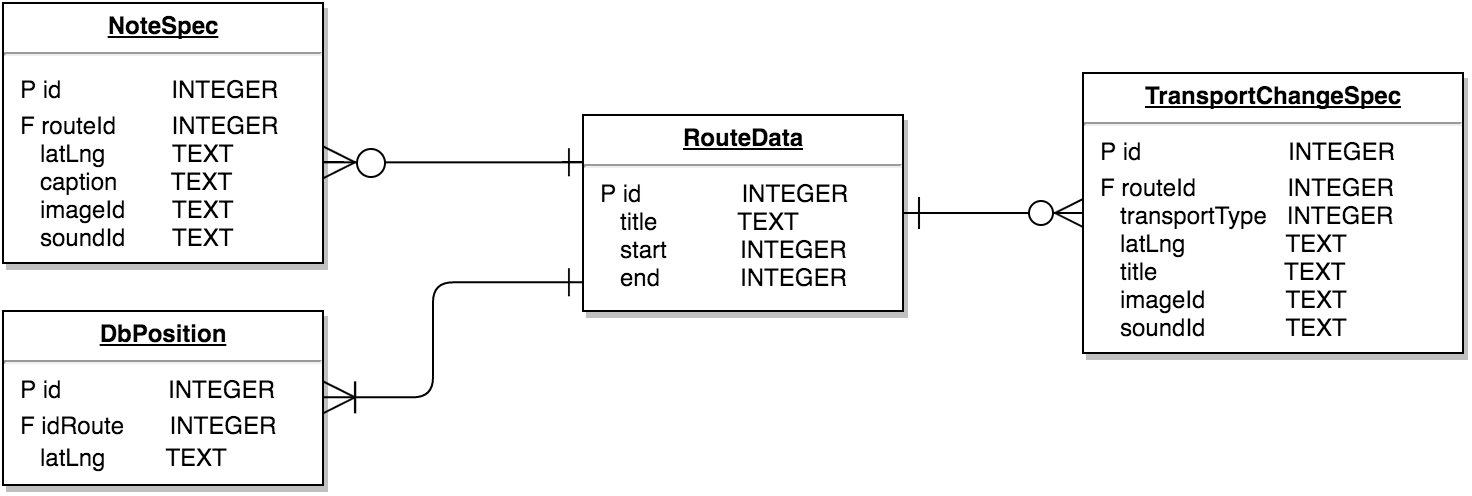
\includegraphics[scale=0.2]{img/db_er.png}
        \caption{ER diagram databázového schéma}
        \label{fig:db_er}
\end{figure}

\subsubsection{Přístup k databázovým datům}
Pro práci s databází byla využita knihovna DBFlow, popsaná v sekci \ref{dbflow}, díky které jsme pro vytvoření
požadované databázové struktury pouze vytvořili třídy pro mapování, které jsme anotovali příslušnými
anotacemi knihovny. Ukládání dat pak probíhá přes tyto objekty a k nim vygenerované adaptéry.
Pro přístup k datům byl použit vzor Repositář\cite{repository}, díky kterému
jsou všechny operace s daty prováděny přes jednu vrstvu a oddělují tak kód práce s daty od zbytku aplikace
jedním rozhraním, za kterým se může nacházet námi implementovaná databázová vrstva, ale také lze toto
pak snadno zaměnit za webovou službu, případně pouze čtení ze souboru.
Bylo vytvořeno rozhraní \texttt{TravelDataRepository}, které můžeme vidět na obrázku \ref{fig:traveldatarepo},
pro které existuje implementace pomocí DBFlow a objekt této implementace je pomocí vkládání závislostí vložen
kdekoliv do aplikace, kde si o to některé třída zažádá, jelikož potřebuje přístup k datům.
Rozhraní vrací všechny hodnoty jako \texttt{Observabe} a tím nechává na klientovi, aby se rozhodl, zda
chce data načíst synchronně, asynchronně, případně umožňuje provést další operace.

\begin{figure}[H]
        \centering
                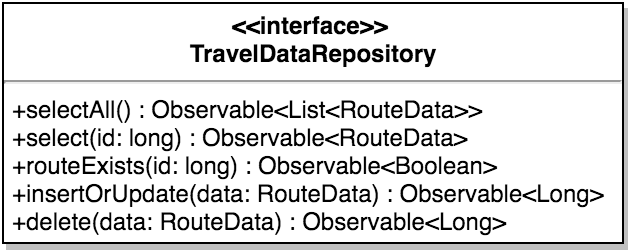
\includegraphics[scale=0.2]{img/repo.png}
        \caption{Rozhraní pro přístup k datům aplikace}
        \label{fig:traveldatarepo}
\end{figure}

\subsubsection{Přístup k souborovým datům}
Jelikož aplikace vytváří i souborová data, je potřeba tato dat ukládat a provázat je s daty v databázi.
Pro naše dva případy fotek a zvukových nahrávek u poznámek bylo použito vygenerování náhodného
objektu \texttt{UUID} při vytváření souboru, soubor se následně v příslušném adresáři pro tento typ
dat podle tohoto identifikátoru pojmenuje a hodnota identifikátoru se uloží do asociovaného sloupce
v databázi. Při načítání dat se tak aplikace například pro obrázky pouze podívá, zda záznam obsahuje
identifikátor obrázku a pomocí získaného identifikátoru získá z manažera obrázků přístup ke konkrétnímu
souboru, který poté může zobrazit uživateli.

\subsubsection{Ukládání nastavení}
Pro uživatelská nastavení, jako například číslo asistenta nebo jeho email, je použit mechanismus Androidu
\texttt{SharedPreferences}, který v našem případě pouze obalujeme naším objektem s přístupovými
metodami pro konkrétní, námi používaná nastavení.


\subsection{Zálohování dat}
Jelikož asistent může strávit poměrně dost času sběrem dat a jejich přípravou pro klienta, je žádoucí chránit data před ztrátou,
poškozením nebo pouze nechtěným smazáním či smazáním odinstalováním aplikace. Aplikace tudíž obsahuje mechanismus pro zálohu všech
dat a to nahraných cest s poznámkami, upozorněními na změnu cesty, fotkami a nahrávkami.

Pro fungující zálohování je nutné přiřadit uživateli identitu a tu rozpoznávat a ověřovat pro přiřazení případná zálohy,
mít k dispozici webové úložiště, komunikovat s ním a porovnávat informace z něj získané s aktuálními daty,
což je poměrně komplexní úkol a vlastní implementace by
vyžadovala vlastní server, hosting a zejména registraci uživatel, což by v případě mentálně postižených klientů
přineslo další složitost do aplikace a nutilo by klienta pamatovat si další uživatelské jméno a heslo.

Tento problém byl vyřešen využitím OAuth2\footnote{Více o OAuth2 se můžeme dozvědět v \cite{oauth2}.}
autorizace přes připojený Google účet na zařízení a API Google Drive nebo česky Disk,
 které je součástí Google Play Services a na zařízení uživatele, který si naši aplikací stáhnul z obchodu Play,
 jsou tato API k dispozici.
V Google vývojářské konzoli je napřed nutné aktivovat využití Google Drive API pomocí jména balíčku aplikace a SHA-1 heše
certifikátu, kterým je podepsáno APK aplikace. Na stejném místě lze také nastavit popis, který se pro aplikaci
uživateli zobrazí, když si prohlíží, které aplikace má ke svému Disku připojeny.
Díky API Google Drive je odpovědnost synchronizace dat přesunuta na služby Googlu a pomocí
OAuth2 se využívá existující účet, čímž se odstraňuje nutnost uživatele zakládat a pamatovat
 další identitu a nám zcela eliminuje nutnost starat se o synchronizaci mezi zařízeními a správu jakýchkoliv účtů.
 Uživatel musí při prvním vytvoření zálohy potvrdit, že souhlasí, aby naše aplikace používala jeho Disk.
 API s tímto počítá a při pokusu o vytváření souborů při nutnosti autorizace sám nabídne ke zobrazení
 dialog pro uživatele a následně vrátí výsledek, zda uživatel službu povolil.

 Data záloh jsou ukládána do tzv. appfolderu\cite{driveappfolder}, což je privátní úložiště aplikace
 a uživatel poté v nastavení svého Disku vidí,
  která aplikace tuto službu využívá a kolik dat zabírá, nevidí však konkrétní data.
  Uživatelův pohled po připojení aplikace a zálohování dat můžeme vidět na obrázku~\ref{fig:connecteddrive}.

\begin{figure}[H]
        \centering
                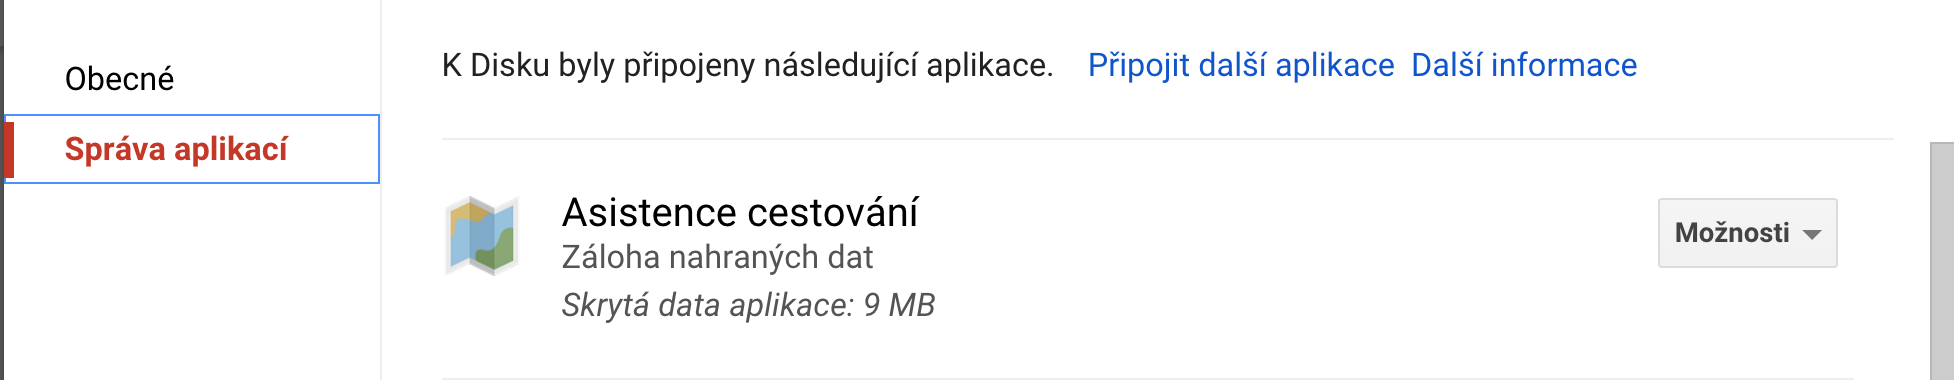
\includegraphics[scale=0.3]{img/connectedDrive.png}
        \caption{Uložená data aplikace na Google Drive}
        \label{fig:connecteddrive}
        \centering Zdroj: \url{https://drive.google.com/drive/my-drive}
\end{figure}

\subsubsection{Záloha}
Pro vytvoření zálohy bylo za účelem minimalizace závislosti na Google Drive API zvoleno vytvoření jediného
dočasného ZIP souboru s databází a soubory, který se následně uloží na Disk uživatele. Dočasný soubor se po
vytvoření zálohy smaže a stejně tak předchozí zálohy na disku, pro omezení využívání příliš mnoha místa duplicitami,
jelikož díky fotkám může být zálohový soubor poměrně velký. Diagram vytváření zálohy můžeme vidět na obrázku~\ref{fig:backup}.

\begin{figure}[H]
        \centering
                \includegraphics[scale=0.25]{img/backup.png}
        \caption{Diagram vytváření zálohy}
        \label{fig:backup}
\end{figure}

\subsubsection{Obnovení ze zálohy}
Pokud uživatel požádá o obnovení ze zálohy, vyhledá se pomocí Drive API poslední ZIP soubor zálohy,
rozbalí se do dočasného úložiště, soubory se přesunou do příslušných složek, uzavře se existující
databázové připojení aplikace, nahradí se databázový soubor souborem ze zálohy a připojení se znovu otevře.
Uživatel může následně začít využívat obnovená data.

\subsection{NFC (\textit{Near Field Communication})}
NFC je bezdrátová technologie umožňující komunikaci dvou zařízení na velmi krátké vzdálenosti do 4 cm
rychlostí do 424 kb/s.\cite{nfcforum}  Výměna dat může být aktivována pouhým přiblížením dvou zařízení k sobě
a technologie podporuje zabezpečený přenos dat. Technologii spravuje organizace NFC Forum jejíž logo lze vidět
na obrázku \ref{fig:nfcforumlogo} a její specifikaci lze nalézt v \cite{nfciso}.
NFC dále implementuje specifikaci ISO/IEC 14443 A a B\cite{nfcforum}, což je standard používaný
současnými platebními kartami a jinými čipy, jehož definici můžeme najít v \cite{rfidiso} a díky této
implementaci je plně kompatibilní se současnými platebními terminály a systémy, což nabízí možnost využití zařízení
podporujících NFC jako platebních čipů jelikož oproti klasickým čipům může NFC zařízení uchovávat více informací
a umožňuje například sloučení více platebních karet a bezpečnostních čipů dohromady do jednoho zařízení,
v našem případě mobilního telefonu.

Během posledních pár let se NFC stalo součástí výbavy mnoha chytrých telefonů a velká většina modelů
už nyní tuto funkčnost podporuje a Android nabízí ve svém API podporu pro NFC už od verze 2.3
vydané v roce 2010 a vývojář je tedy odstíněn od všech nízkoúrovňových komunikačních protokolů.
V naší aplikaci využijeme tzv. NFC tagů, což je malý vestavěný čip schopný pomocí NFC uchovat malé množství dat a
následně touto technologií tyto data přečíst. Tagy se dají v současnosti koupit na internetu za desítky
korun a mohou být různých tvarů a barev.

V aplikaci Asistenci Cestování bylo implementováno uložení URL s informací o nahrané cestě. Funkce
pracující s s NFC jsou v aplikaci označeny jednotnou ikonou na obrázku \ref{fig:nfcicon},
která je nejčastěji používána Android aplikacemi.
 Pokud uživatel klepne na ikonu NFC při prohlížení detailu cesty, zobrazí se mu obrazovka s instrukcemi a po přiložení
zapisovatelného NFC tagu je toto URL uloženo do tagu spolu s informací, že právě naše aplikace umí toto URL
rozpoznat. V Android Manifestu je následně definována aktivita s intent filtrem na akci \textit{NDEF\_DISCOVERED},
což systému říká, že při objevení NFC tagu má zařadit naši aplikaci na seznam aplikací, které dokážou
rozpoznat NFC tagy a spolu s námi zapsanou informací do tagu je to právě naše aplikace, která při přiložení
tagu zprávu obdrží, dekóduje URL a podle jeho obsahu spustí navigaci nalezené cesty.

Výsledkem je, že uživateli se při přiložení konkrétního tagu zobrazí připravená navigace pro danou
cestu bez jakékoliv další akce, což značně zjednodušuje používání aplikace, jelikož jinak by pro spuštění navigace
uživatel musel aplikaci spustit, nalézt požadovanou cestu a klepnout na ikonku navigace. Nápadem
 využití je připevnění několika NFC tagů rozlišených barvami vedle dveří bytu klienta a při odchodu na
 cestu uživatel spustí asistenci k cestě přiložením telefonu k požadované barvě.

\begin{figure}[H]
\begin{minipage}{.5\textwidth}
\centering
                
\includegraphics[scale=0.4]{img/nfc-forum-logo.png}
        \caption{Logo organizace NFC Forum}
        \label{fig:nfcforumlogo}
        \centering Zdroj: \url{http://nfc-forum.org/}
\end{minipage}
\begin{minipage}{.5\textwidth}
\centering
                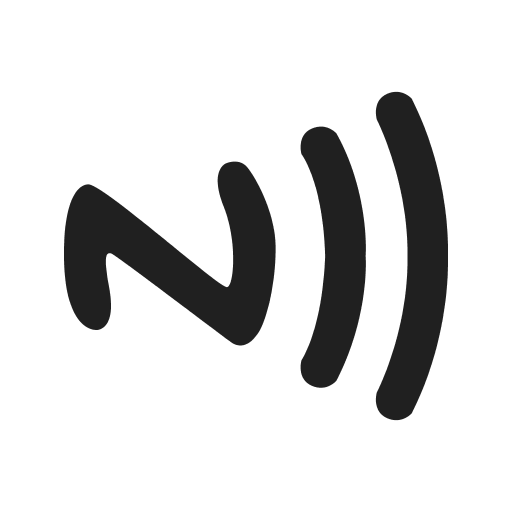
\includegraphics[scale=0.07]{img/nfc-icon.png}
        \caption{Ikona NFC}
        \centering Zdroj: \url{https://materialdesignicons.com/}
        \label{fig:nfcicon}
    \end{minipage}
\end{figure}

\subsection{Publikování aplikace}
Pro publikování aplikace byl zvolen obchod Google Play provozovaný Googlem, což je standardní způsob
publikování Android aplikací. Google Play poskytuje bohaté rozhraní pro správu aplikací, statistiky
instalovaných zařízení, verzí systému používajících naší aplikaci, reporting chyb a další. Poskytuje také
nástroje pro propagaci aplikace a v neposlední řadě správu verzí aplikace, grafiky a popisů
vztahujících se k aplikaci. Naše aplikace je v tomto obchodě samozřejmě přístupná zdarma, nicméně
je možné publikovat placené aplikace, kde Google Play řeší distribuci do všech vybraných států a za služby
prodeje si strhává provizi 30\%.

Od nedávna obchod podporuje také otevřené alfa a beta testování, pro které lze uživatele zvát anonymně
pouze za pomoci odkazu. Dříve bylo nutné zakládat vývojářské skupiny a přidávat do nich jmenovitě
lidi, což bylo zdlouhavé a pracné. Po odeslání testovacího odkazu se obchod uživatele pouze zeptá,
zda se chce stát testerem a může si následně stáhnout aplikaci, která je jinak pro veřejnost nepřístupná
Pro původní testování aplikace je využit alfa kanál pouze pro úzký okruh uživatelů, následně následuje beta
kanál pro širší testování a odhalení chyb, které stále nejsou mezi všemi uživateli, nicméně uživatelů je
dost na to, aby se chyby projevily. Po tomto kroku následuje povýšení aplikace do produkce, kde je již
veřejně přístupná a může si ji stáhnout i náhodný uživatel, který aplikaci v obchodě objeví. Ukázku
vhledu publikování aplikace pro obchod Play můžeme vidět na obrázku \ref{fig:playconsole}.

Existují také alternativní obchody, ze kterých si lze stáhnout aplikace, z nichž největší je obchod Amazonu,
nicméně podíl těchto obchodů je minoritní a pokud uživatel chce tyto alternativní obchody používat,
musí na zařízení v nastavení povolit instalaci aplikací z neznámých zdrojů, což je značné bezpečnostní
riziko. Dříve často diskutovaná chabá bezpečnost systému byla často zapříčiněna uživateli využívající
tyto alternativní obchody, kde neexistovala verifikace uživatele nebo obsahu a mohl na ně prakticky
kdokoliv nahrát škodlivou aplikaci zdarma tvářící se jako některá z populárních placených aplikací.

Pro publikování na Google Play je nutné aplikaci podepsat produkčním certifikátem, který byl
vygenerován s platností na 50 let a je uložen mimo systém správy verzí, jelikož se jedná o esenciální
bezpečnostní prvek, neboť při jeho zcizení by nabyvatel mohl publikovat aplikaci se stejným podpisem
jako naše aplikace a distribuovat tak škodlivý kód pod naším jménem.

\begin{figure}[H]
        \centering
                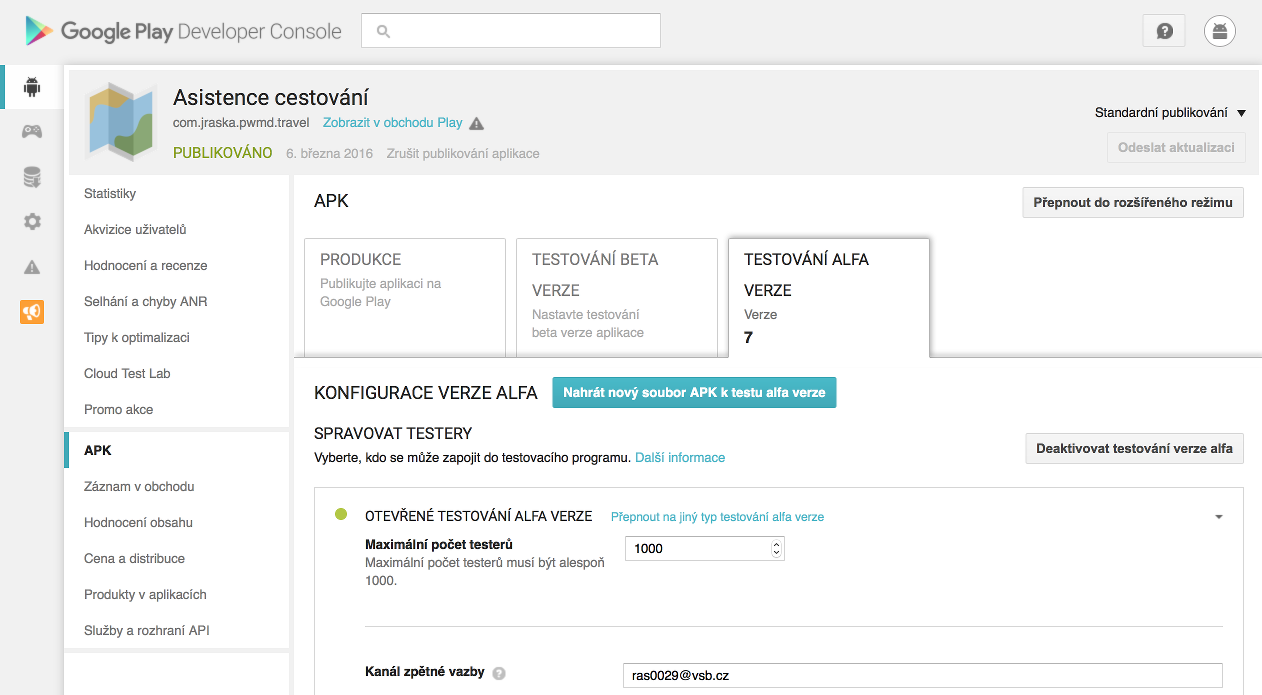
\includegraphics[scale=0.5]{img/playconsole.png}
        \caption{Rozhraní publikování aplikace na Google Play}
        \label{fig:playconsole}
\end{figure}


\section{Testování aplikace}
Po nasazení aplikace bylo potřeba vychytat všechny možné problémy a nedostatky, které se mohly projevit
a zhoršit uživatelskou zkušenost s aplikací.

\subsection{Optimalizace výkonu}
Jedno z nejstarších pravidel programování je neoptimalizovat zbytečně dopředu na základě odhadu,
jelikož programátoři jsou v těchto odhadech většinou velmi špatní. Během vývoje byl přesto na efektivní
implementaci kladen důraz a všechny potencionálně delší operace byly prováděny asynchronně mimo vlákno
uživatelského rozhraní, jelikož pro optimální uživatelský zážitek je potřeba stihnout vše ve vlákně
uživatelského rozhraní do 16ms\cite{perf}.

Aplikace, která chce toto uživateli umožnit, musí do asynchronních operací přesunou většinu svých déle
trvajících operací, což bylo v našem případě zejména čtení a ukládání do databáze, jelikož se v tomto
 případě komunikuje se souborovým systémem, ale také například komunikaci s API Google Play Services,
 kde může dojít k ověřování využívání API přes internet což už z principu znamená poměrně dlouhou
 prodlevu. Pro implementaci těchto operací byla použita knihovna RxAndroid, popsaná v sekci \ref{rxandroid}
 a aplikace se poté stává mnohem rychlejší a zejména odezva uživatelského rozhraní
 na akce uživatele je téměř okamžitá.

\subsubsection{Pomalé načtení úvodní obrazovky s cestami}
 Při testování se z počátku na pomalých zařízeních projevovalo pomalé načítání úvodní obrazovky se
 seznamem cest. Bylo tedy využito profilovacího nástroje Traceview, který je součástí Android SDK
  a je možné jej využít pro zaznamenání a zobrazení provádění metod za běhu. Výstup profilování kódu
  mezi synchronním načtením v metodě \texttt{refreshRoutes} a zobrazením výsledku v uživatelském rozhraní
  můžeme vidět na obrázku \ref{fig:syncroutes}, kde je výstup hlavního vlákna uživatelského rozhraní.
  Z důvodu předcházení nedorozumění upozorňuji, že profilovací výstupy jsou lokalizovány
  v angličtině a tudíž je čárka brána jako oddělovač tisíců, nikoliv jako oddělovač desetinných míst,
  pro který je používána tečka. 88,509$\mu$s ve výstupu tedy znamená 88ms, 509$\mu$s.

  \begin{figure}[H]
          \centering
                  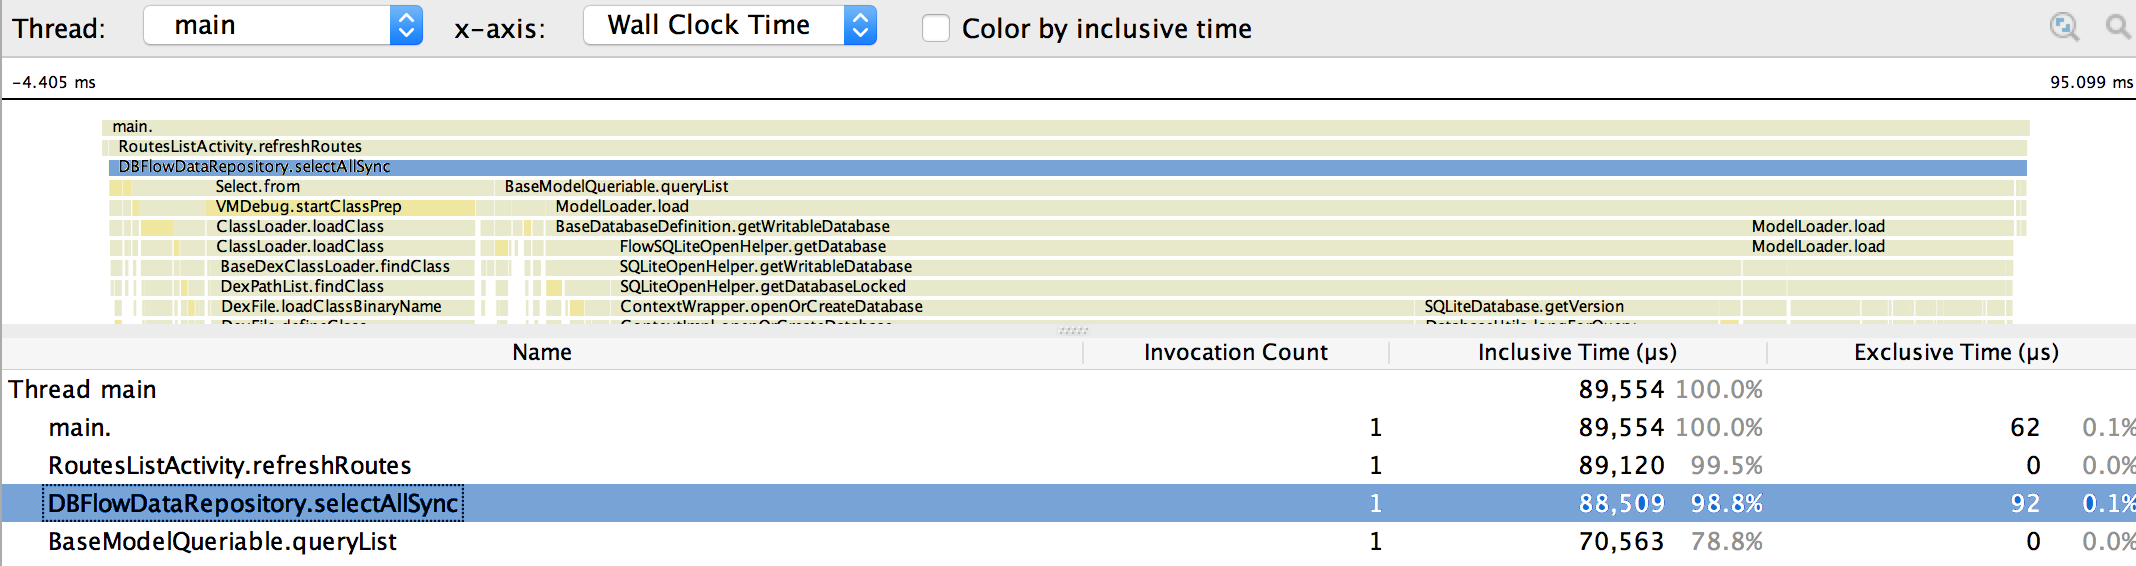
\includegraphics[scale=0.38]{img/SyncRoutesMainThread.png}
          \caption{Výstup profilování synchronního načítání cest}
          \label{fig:syncroutes}
  \end{figure}

  Jak na obrázku \ref{fig:syncroutes} můžeme vidět, metoda \texttt{selectRoutesSync} zabírá 98.8\%
  z celého načítání a zobrazení dat a trvá více než 88ms, což sice nemusí být kritické,
  nicméně se jedná pouze o čas na testovacíma zařízení a na některých pomalejších zařízeních
  s například starým typem SD karty může být tento čas mnohem vyšší a uživateli
  již může přivodit pocit pomalé odezvy. Na časové ose také můžeme identifikovat důvody pomalého
  zobrazení při prvním načtení. Při prvním volání se totiž v metodě \texttt{ClassLoader.loadClass}
  načítají do paměti nahrávají do paměti všechny třídy potřebné pro načtení dat z databáze,
  což jsou v tomto případě naše mapovací třídy reprezentující data v paměti, třídy ORM knihovny
  DBFlow a také třídy samotného frameworku Android pro přístup k SQLite databázi. Významnou
  roli hraje také otevírání databáze, které proběhne v metodě \texttt{SQLiteOpenHelper.getWritableDatabase}
  a opět probíhá při prvním přistupu k databázi a samotné načtení dat, probíhající v metodě
 \texttt{ModelLoaer.load} je v tomto případě minoritním konzumentem času vlákna.

 Pro optimalizaci bylo tedy využito asynchronního načtení, kde se pomocí využití knihovny RxAndroid
 přesunulo volání těchto metod do jiného vlákna a následně se do hlavního vlákna publikoval
 pouze výsledek asynchronní operace. Implementaci takového volání jsme mohli vidět na ukázce kódu
 \ref{rxmainthreaddeliver} na straně \pageref{rxmainthreaddeliver}.

 Při opětovném profilování, jehož výstup můžeme vidět na obrázku \ref{fig:asyncroutesmainthread},
 se nám povedlo významně snížit čas volání metody \texttt{refreshRoutes} na mnohem lepších 6.5ms
 a majoritní část práce hlavního vlákna tvoří vykreslování uživatelského rozhraní v metodě
 \texttt{doFrame}, což je přesně to, čeho jsme chtěli dosáhnout.

 \begin{figure}[H]
           \centering
                   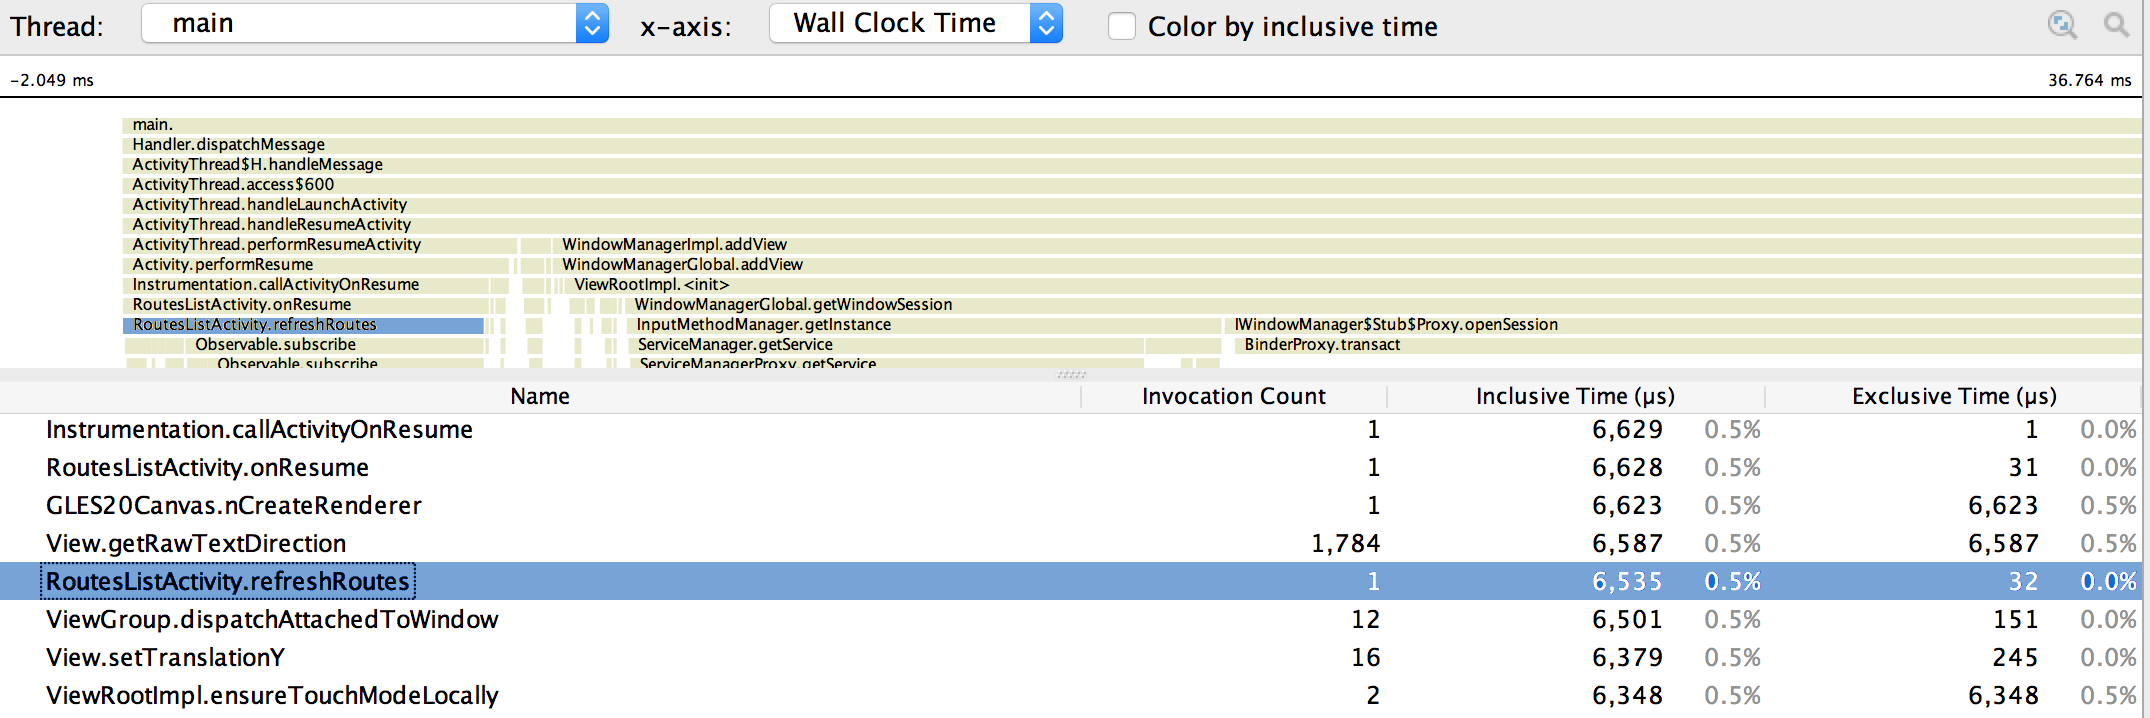
\includegraphics[scale=0.38]{img/AsyncRoutesMainThread.png}
           \caption{Výstup profilování hlavního vlákna asynchronního načítání cest}
           \label{fig:asyncroutesmainthread}
   \end{figure}

Ze stejného profilovacícho výstupu se lze přepnout do záznamů z asynchronního vlákna, který je
na obrázku \ref{fig:asyncroutesrxthread}, kde můžeme vidět, že provádění metody
\texttt{selectRoutesSync} nyní trvá 130ms, nicméně se tak děje v pracovním vlákně aplikace a uživatel
 tak nezaznamená zaseknutí uživatelského rozhraní při zobrazování obrazovky a po prodlevě načítání
 se mu pak do připraveného uživatelského rozhraní pouze zobrazí samotné cesty.

    \begin{figure}[H]
              \centering
                      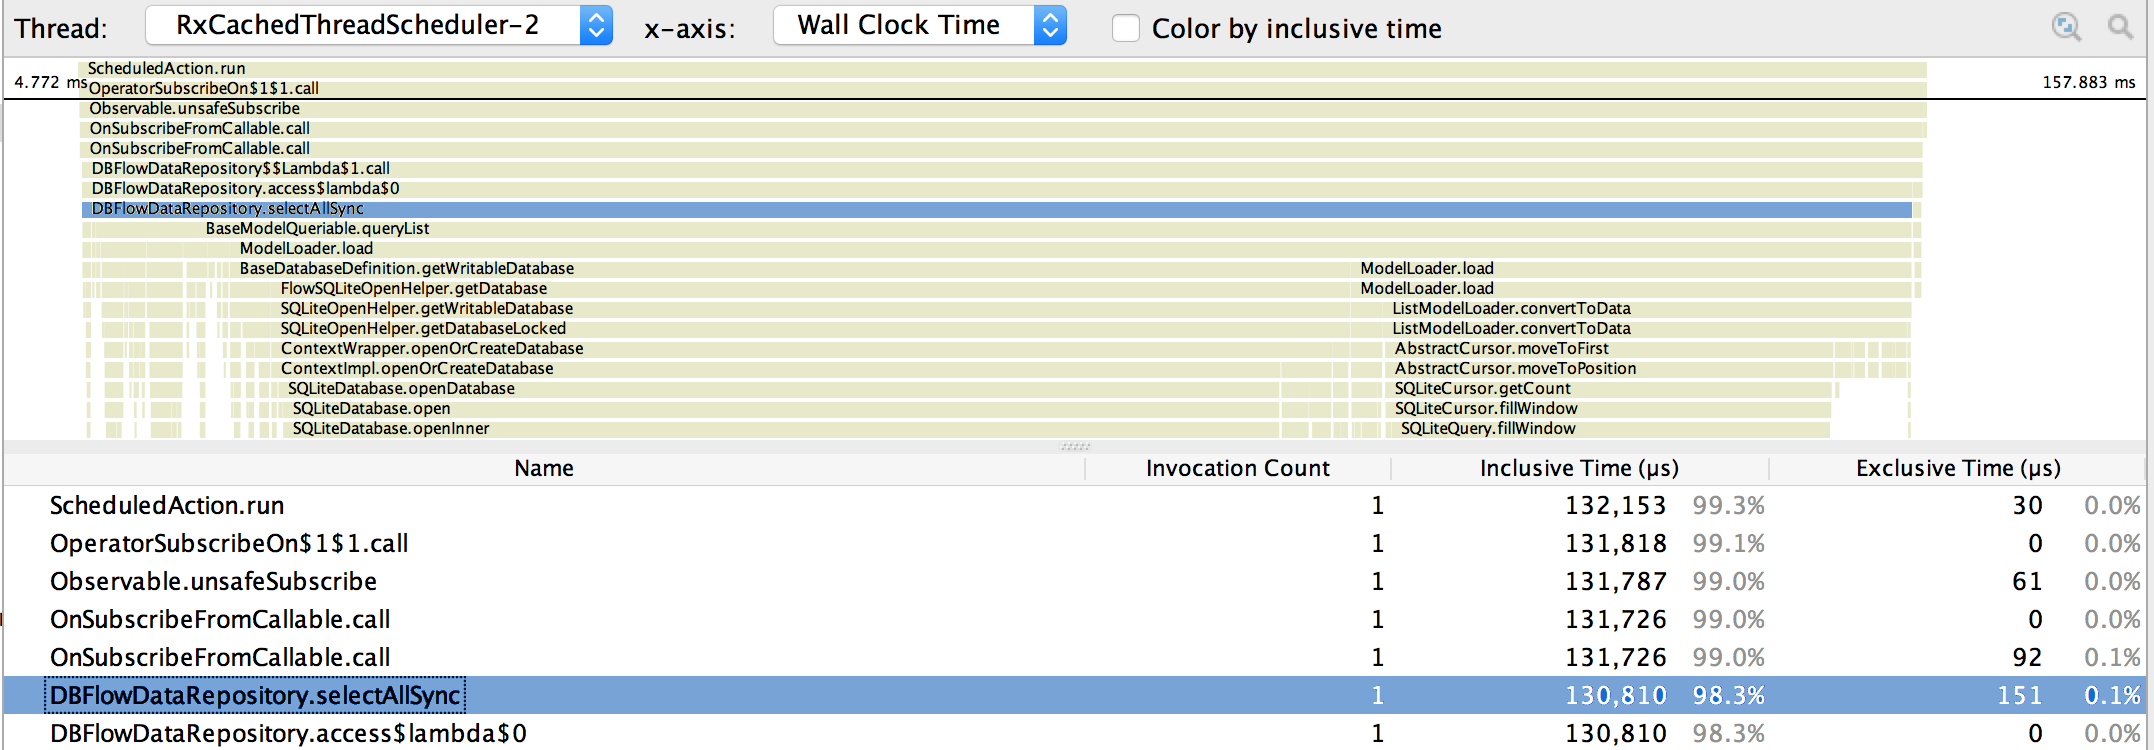
\includegraphics[scale=0.38]{img/AsyncRoutesRxThread.png}
              \caption{Výstup profilování pracovního vlákna asynchronního načítání cest}
              \label{fig:asyncroutesrxthread}
      \end{figure}

Pro pomalé zařízení byl tedy problém se zablokováním uživatelského rozhraní takto vyřešen. Podobné
profilování bylo provedeno preventivně i u ostatních obrazovek, neboť výstup profilovací nástroje může
velmi často odhalit nejen výkonnostní problémy, ale také chyby. Žádné zásadní problémy nebyly
v době psaní této práce objeveny.

\subsubsection{Průběžné monitorování výkonu}
Jak již bylo řečeno, není nevyžádaná optimalizace doporučeným postupem, jelikož je optimalizovaný kód
často složitější a hůře čitelný. Během vývoje byl proto využit nástroj
Hugo\footnote{Dostupné na https://github.com/JakeWharton/hugo (10.4.2016)}, který pouhým
anotováním metody anotací \texttt{@DebugLog} začne do logu zařízení vypisovat informace o vstupech metody,
jejím výstupu a také čas provádění. Činí tak pouze v ladícím režimu, což je to, co od něj požadujeme
a aplikace používaná finálními uživateli tedy není tímto logováním nijak ovlivněna. V projektu byly
takto anotovány všechny potencionálně pomalé metody a po vyfiltrování těchto metod ve výstupu logů se
tak lze snadno podívat, které metody opravdu zabírají více času a umožňuje nám ujistit se, že jsou
tyto metody spouštěny v asynchronním vlákně. Ukázku použití můžeme vidět na ukázce kódu \ref{hugoshowcase},
kde zjistíme, že načtení detailu cesty trvá 248ms, což by již bylo velmi problematické provádět v uživatelském
vlákně, nicméně k naší spokojenosti také vidíme, že se toto provádí v asynchronním vlákně knihovny RxAndroid.

\begin{lstlisting}[label=hugoshowcase,caption=Využití nástroje Hugo pro výpisy informací o prováděných metodách]
  @DebugLog
  private RouteData selectSync(long id) { ... }
            ▼                ▼
  V/DBFlowDataRepository:  selectSync(id=4) [Thread:"RxCachedThreadScheduler-1"]
  V/DBFlowDataRepository:  selectSync [248ms] = RouteData(_deletedId=0, _id=4, _start...
\end{lstlisting}

\subsection{Pády aplikace}
Jedním z nejnepříjemnějších problémů, co může uživatele potkat, je pád aplikace a neslavné dialogové
okno s dotazem, zda chceme aplikaci ukončit. Bývá poté velmi těžké uživatele přesvědčit, aby se
do aplikace vrátil. Při každém vydávání verze byly proto vždy otestovány všechny hlavní scénáře,
kterými aplikace prochází, nicméně i přesto se můžou chyby dostat do produkce a je důležité se
 o nich dozvědět.

 Pro tyto účely se opět používají služby obchodu Google Play a knihovny Google Play Services instalované
 na zařízení. Pokud nastane za běhu aplikace výjimka a aplikace spadne. Zobrazí se uživateli nabídka
 k odeslání zpětné vazby spolu s informacemi o chybě. testovací uživatelé byli instruováni toto udělat
 a vzhledem k dřívějším testům byla takto nahlášena pouze jedná výjimka.

 Nahlášené chyby si lze poté prohlédnou v konzoli obchodu Google Play, kde se nahrají také další
 důležité informace o zařízení, jako verze systému, výrobce, typ zařízení a zejména trasování zásobníku
 chyby, podle kterého je snadno možné chybu odhalit. Ukázku nahlášené chyby můžeme vidět na obrázku
 \ref{fig:anr}.

   \begin{figure}[H]
               \centering
                       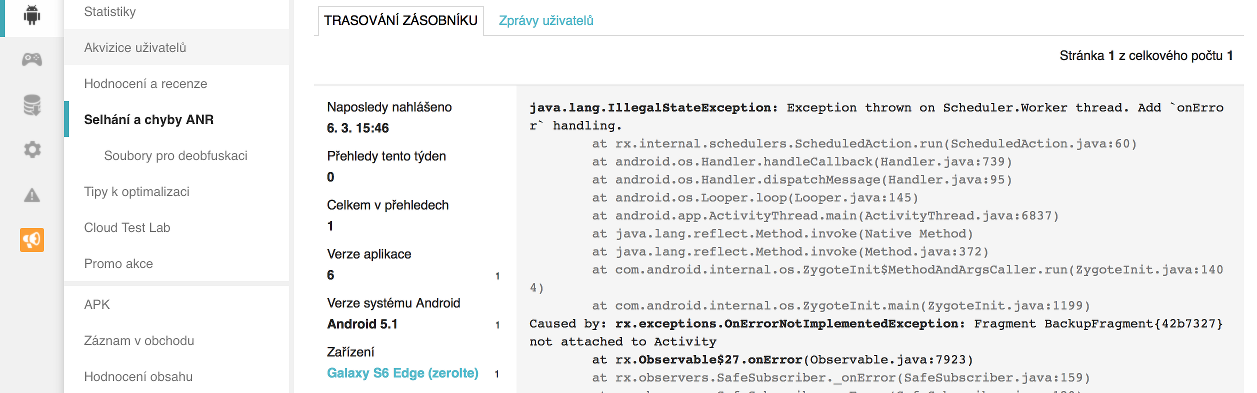
\includegraphics[scale=0.7]{img/anr.png}
               \caption{Nahlášený pád aplikace v konzoli Google Play}
               \label{fig:anr}
       \end{figure}

Při procházení výpisu bylo zjištěno, že chyba je způsobena voláním metod fragmentu pro získání textových zdrojů
 vyžadujících připojenou aktivitu, nicméně volání této metody přišlo v okamžiku, kdy aktivita rotovala
a tudíž byl fragment již z aktivity odstraněn, což vedlo k nahlášenému selhání.

Chyba byla vyřešena kontrolou stavu a získáváním textových zdrojů již při vytváření fragmentu,
kdy máme jistotu, že je fragment k aktivitě správně připojen. Po nahrání opravné verze na Google Play
byla nové verze distribuována během pár hodin, byla tak opravena a jak můžeme vidět na obrázku
\ref{fig:anr}, objevila se pouze jednou.

\subsection{Napovídání uživateli}
Jak se během testování ukázalo, někteří uživatelé si při prvním spuštění obrazovky nahrávání nebyli
 jistí, čím mají začít a přesto, že jediné tlačítko, na které je v tu chvíli možné klepnout je
 tlačítko nahrávání s ikonou, kterou jsme mohli vidět na obrázku \ref{fig:nahravanicestyicon}
 a při podržení prstu na tlačítku s touto ikonou se zobrazí popis akce.

 Bylo proto potřeba při prvním spuštění uživateli ještě výrazněji ukázat, kde má na této obrazovce začít.
 Pro tento účel bylo použito překrytí celé obrazovky poloprůhlednou vrstvou, na které je napsán text, který radí
 uživateli, že má klepnout na tlačítko nahrávání a toto tlačítko se nachází v kruhové oblasti nápovědy, která je
 jako jediná v ten okamžik průhledná. Uživateli se toto zobrazí pouze pokud obrazovku otevře poprvé
 a upozornění se skryje, pokud provede jakoukoliv uživatelskou akci a informace o tom, že nápověda byla uživateli
 již zobrazena se uloží do nastavení zařízení. Zobrazení nápovědy můžete vidět na obrázku \ref{fig:nahravaninapoveda}.

  \begin{figure}[H]
            \centering
                    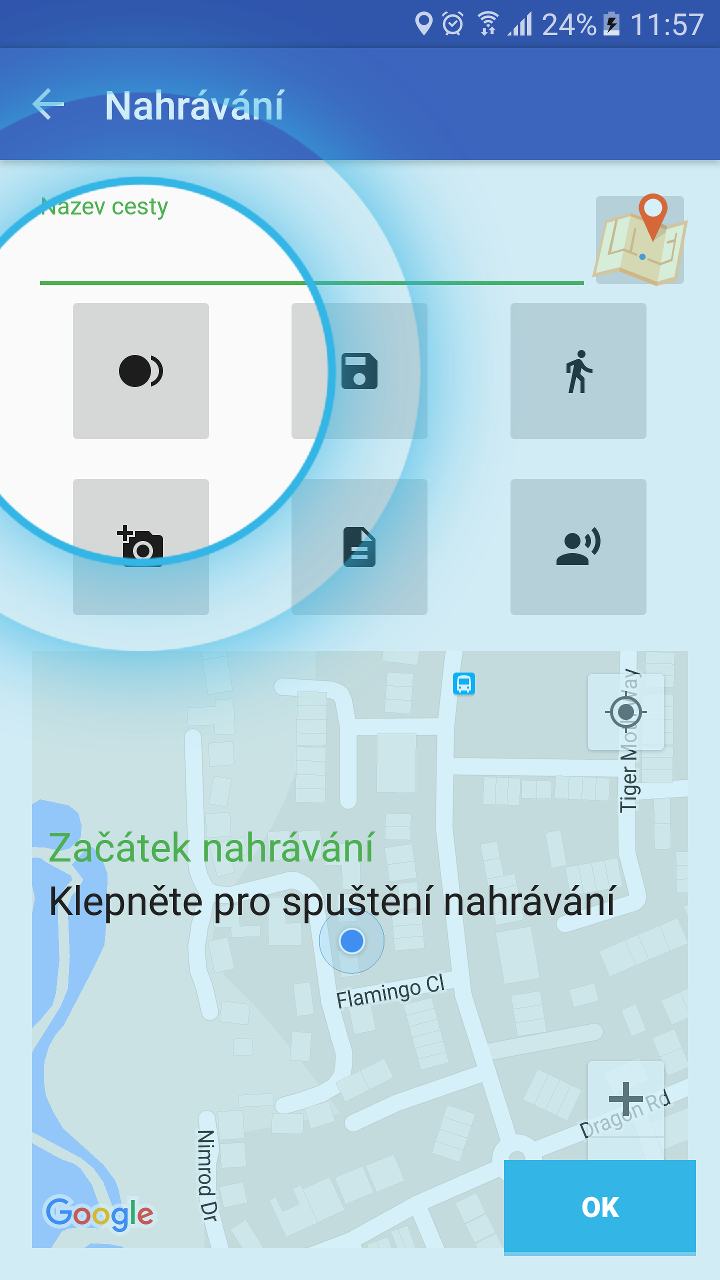
\includegraphics[scale=0.14]{img/screen/nahravaninapoveda.png}
            \caption{Zobrazení nápovědy uživateli}
            \label{fig:nahravaninapoveda}
    \end{figure}



\section{Závěr}
V práci jsme si ukázali průběh návrhu mobilní aplikace od diskuze zadání po funkční a grafický návrh.
Následně byly vybrané části implementovány a v rámci implementace jsme si taky předvedli použití mnoha knihoven a technik
pro efektivní vývoj a stabilní Android aplikace. Byla diskutována architektura a metodika vývoje Android aplikace,
která byla následně využita k implementaci. Aplikace byla následně publikována a otestována několika uživateli pro
 získání zpětné vazby a vyladění nedostatků, přičemž je stále co zlepšovat a rozšiřovat.

Asistence cestování mentálně postižených se ukázala jako mimořádně zajímavý a také obtížný úkol.
Pokusil jsem se poskytnout lidem s mentálním postižení a jejich asistentům nový nástroj, který by
jim mohl v jejich často nelehké situaci pomoci a věřím, že některým také pomůže. Práce mi dala
nový rozhled o lidech kolem nás a také spoustu nových vývojářských zkušeností, které
jistě budu moci brzy zúročit v profesním životě.

V problematice této mobilní aplikace pro asistenci cestování je stále spoustu věcí k vylepšování
a v případě používání aplikace uživateli může pokračovat i její vývoj, případná implementace serverové části.
Vzhledem k otevřenosti kódu aplikace může v mé práci kdokoliv pokračovat a díky použití
aktuálních knihoven a nástrojů může aplikace posloužit také jako ukázka využití některé z knihoven
a již jsme jí také za tímto účelem použil.

\begin{thebibliography}{99}


\bibitem{komunikace}{INCLUSION EUROPE}
\textit{Zásady úspěšné komunikace s lidmi s mentálním postižením: Doporučené přístupy k lidem
s mentálním postižením v rámci jejich celoživotního vzdělávání i mimo něj}, {Praha, 2009}
\newline
(Dostupné dne 10.4.2016 na \url{http://www.inclusion-europe.com/pathways2/images/CZ_Recommendations.pdf})


\bibitem{perf}{SILLARS, DOUG}
\textit{High Performance Android Apps}. {O'Reilly Media, Inc., 2015}
\newline(Dostupné dne 10.4.2016 na \url{https://www.safaribooksonline.com/library/view/high-performance-android/9781491913994/}, )

\bibitem{bestpracticesfuturice}{FUTURICE OY}
\textit{Best practices in Android development}. {Futurice Oy, 2016}
\newline(Dostupné na \url{https://github.com/futurice/android-best-practices}, 10.4.2016)


\bibitem{androiddevelopers}{GOOGLE, INC.}
\textit{Android API Guides}. {Google, 2016}
\newline(Dostupné na \url{http://developer.android.com/guide/index.html}, 10.4.2016)

\bibitem{materialdesign}{GOOGLE, INC.}
\textit{https://www.google.com/design/spec/material-design/}. {Google., 2015}
\newline(Dostupné na \url{https://www.google.com/design/spec/material-design/}, 10.4.2016)

\bibitem{androidcentral}{MOBILE NATIONS}
\textit{Android History}. {Android Central, 2016}
\newline(Dostupné na \url{http://www.androidcentral.com/android-history}, 10.4.2016)

\bibitem{mvcxmvp}{TECHYOURCHANCE}
\textit{Model View Controller (MVC) and Model View Presenter (MVP) architectural patterns in Android}. {TechYourChance, 2015}
\newline(Dostupné na \url{http://bit.ly/25RbZ4L}, 9.4.2016)

\bibitem{ioc}{FOWLER, MARTIN}
\textit{Inversion of Control Containers and the Dependency Injection pattern}. {Martin Fowler, 2004}
\newline(Dostupné na \url{http://www.martinfowler.com/articles/injection.html}, 10.4.2016)

\bibitem{solid}{OLORUNTOBA, SAMUEL}
\textit{S.O.L.I.D: The First 5 Principles of Object Oriented Design}. {Scotch.io, 2015}
\newline(Dostupné na \url{https://scotch.io/bar-talk/s-o-l-i-d-the-first-five-principles-of-object-oriented-design}, 10.4.2016)

\bibitem{repository}{LALANDA, PHILLIPE}
\textit{Shared repository pattern}. {Pattern Languages of Programs'98, 1998}
\newline(Dostupné na \url{http://www.hillside.net/plop/plop98/final_submissions/P24.pdf}, 10.4.2016)

\bibitem{oauth2}{D. HARDT, ED.}
\textit{The OAuth 2.0 Authorization Framework}. {Microsoft, 2012
\newline(Dostupné na \url{https://tools.ietf.org/html/rfc6749}, 10.4.2016)}

\bibitem{gms}{GOOGLE, INC.}
\textit{Overview of Google Play Services}. {Google, 2016
\newline(Dostupné na \url{https://developers.google.com/android/guides/overview}, 10.4.2016)}

\bibitem{sqlitetypes}{SQLITE}
\textit{Datatypes In SQLite Version 3}. {SQLite
\newline(Dostupné na \url{https://www.sqlite.org/datatype3.html}, 10.4.2016)}


\bibitem{bspline}{MAISSAN, CHRIS}
\textit{Curves and Splines}.
\newline(Dostupné na \url{https://maissan.net/articles/simulating-vines/2}, 10.4.2016)



\bibitem{driveappfolder}{GOOGLE, INC.}.
\textit{Drive API for Android}. {Prosinec 2015,
\newline(Dostupné na \url{https://developers.google.com/drive/android/appfolder}, 10.4.2016)}

\bibitem{nfcforum}{NFC FORUM}.
\textit{About the Technology}. {2016,
\newline(Dostupné na \url{http://nfc-forum.org/what-is-nfc/about-the-technology/}, 10.4.2016)}

\bibitem{nfciso}{ISO/IEC}.
\textit{ISO/IEC 18092}. {2013,
\newline(Dostupné na \url{https://www.iso.org/obp/ui/#iso:std:56692:en}, 10.4.2016)}


\bibitem{rfidiso}{OPEN PCD}.
\textit{ISO14443}. {
\newline(Dostupné na \url{http://www.openpcd.org/ISO14443}, 10.4.2016)}

\bibitem{android4}{GRANT, ALLEN}.
\textit{Android 4}. {Computer Press, 2013, překlad Mužík Jakub}

\bibitem{nfctech}{NFCTECH.CZ}.
\textit{Web nfctech.cz}. {
\newline(Dostupné na \url{http://www.nfctech.cz}, 10.4.2016)}

\end{thebibliography}

  \appendix

  \section{Zdrojové kódy}
  Kódy celé aplikace a všech dalších zdrojů, včetně zdrojového \mbox{\LaTeX}
  souboru k tomuto dokumentu
   lze nalézt na přiloženém CD, případně veškeré soubory
  projektu jsou v aktuální verzi dostupné na adrese \url{https://github.com/jraska/Diploma-Thesis}(29.4.2016),
  kde je verze uložená na CD dostupná pod tagem \texttt{thesis-release} v sekci releases.

\end{document}